\documentclass{article}

\usepackage{graphicx} % Per immagini
\usepackage{tabularx} % Per creare tabelle styfel
%\setlength\parindent{0pt} % Rimuove indendazioni
\usepackage[utf8x]{inputenc} %serve per i simboli utf8x

\usepackage{subcaption} %serve per mettere le subfigure ESCLUDE SUBFIG

\usepackage{times} % Uncomment to use the Times New Roman font
\usepackage{siunitx}
\usepackage{textgreek}
\usepackage{multirow}
\usepackage{float} %serve per mettere le immagini in posizione Here
%\usepackage{subfig} %serve per mettere più figure in colonna o in riga
\usepackage[a4paper,total={170mm,257mm},left=25mm,right=25mm,bottom=35mm]{geometry} % per il layout


\begin{document}

	\title{RELAZIONI DI LABORATORIO DI BIOLOGIA MOLECOLARE}

	\author{Litterini S. \\Giulio B. \\Cracco A.\\Buzzolan T. }

	\date{\today}

	\maketitle

	\vspace{1.5cm}

	\large{\textbf{ELENCO DELLE RELAZIONI :}}
	\vspace{0.5cm}

	\begin{enumerate}

		\item Minipreparazione di DNA plasmidico
		\item Estrazione dell'RNA totale con TRIZOL
		\item Preaparazione TAE 50X e restrizione del DNA
		\item Polymerase Chain Reaction (PCR)
		\item Praparazione terreno LB, cellule competenti e piastre LB-agar
		\item Trasformazione delle cellule di E. coli XL1 Blue
		\item Allestimento culture cellulari
		\item Utilizzo delle culture cellulari umane in analisi molecolari e morfologiche
		\item Estrazione RNA con kit su colonnina Qiagen: Retrotrascrizione in cDNA
		\item Amplificazione RealTime PCR ed Estrazione delle proteine totali
		\item SDS-PAGE delle proteine estratte
		\item Separazione cellulare su gradiente di ficoll

	\end{enumerate}

	\newpage

	%STRUMENTI

	\large{\textbf{STRUMENTI UTILIZZATI NELLE ESPERIENZE :}}

		\vspace{0.5cm}

		Prima di entrare in un laboratorio, bisogna come prima cosa, adeguarsi del materiale necessario
		per poter eseguire i vari lavori in tutta \textbf{sicurezza e praticità}, per questo abbiamo bisogno di munirci
		sei seguenti strumenti:

	\begin{enumerate}

		\item In primis : guanti in lattice

		\begin{figure}[H]

			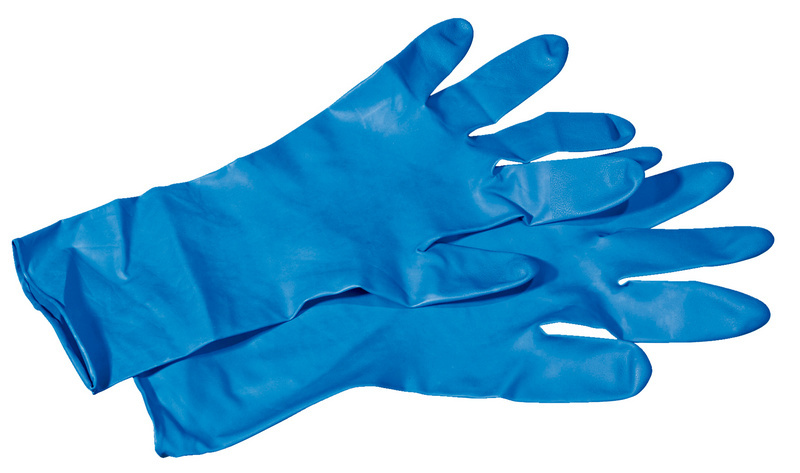
\includegraphics[width=0.5\textwidth]{./immagini/guanti.jpg}
			\caption{Guanti in lattice usa e getta da laboratorio con lo scopo di proteggere le mani da agenti di vario tipo, principalmente dannosi alla pelle,
			oppure per proteggere i materiali utilizzati.}
			\label{guanti}

		\end{figure}

		\vspace{0.5cm}


		\item Camice:

		\begin{figure}[H]

			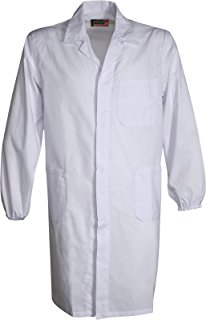
\includegraphics[width=0.4\textwidth]{./immagini/camice.jpg}
			\caption{Camice bianco da laboratorio, utilizzato in tutti i laboratori per esigenze di igene e pulizia.}
			\label{camice}

		\end{figure}

		\vspace{0.5cm}


		\item Cappa biologica:

		\begin{figure}[H]

			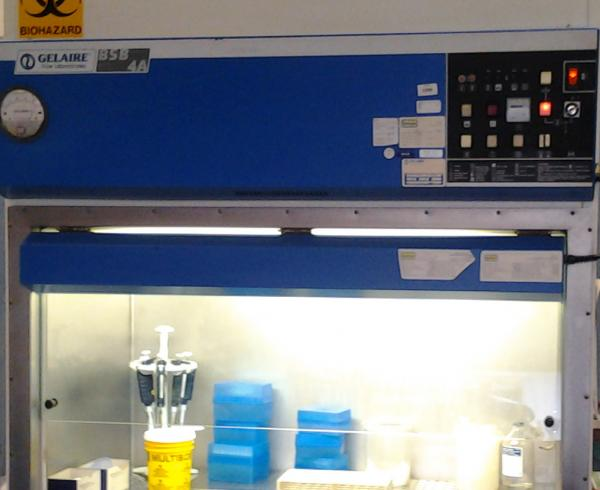
\includegraphics[width=0.4\textwidth]{./immagini/cappa_biologica.jpg}
			\caption{La cappa biologica o cappa a flusso laminare, è una cappa utilizzata in ambito biologico per la protezione di chi maneggia elementi
			biologici, ed elimina la possibilità di contaminazioni crociate, consentendo un lavoro in condizioni di sterilità.}
			\label{cappa_biologica}

		\end{figure}

		\vspace{0.5cm}


		\item Cappa chimica:

		\begin{figure}[H]

			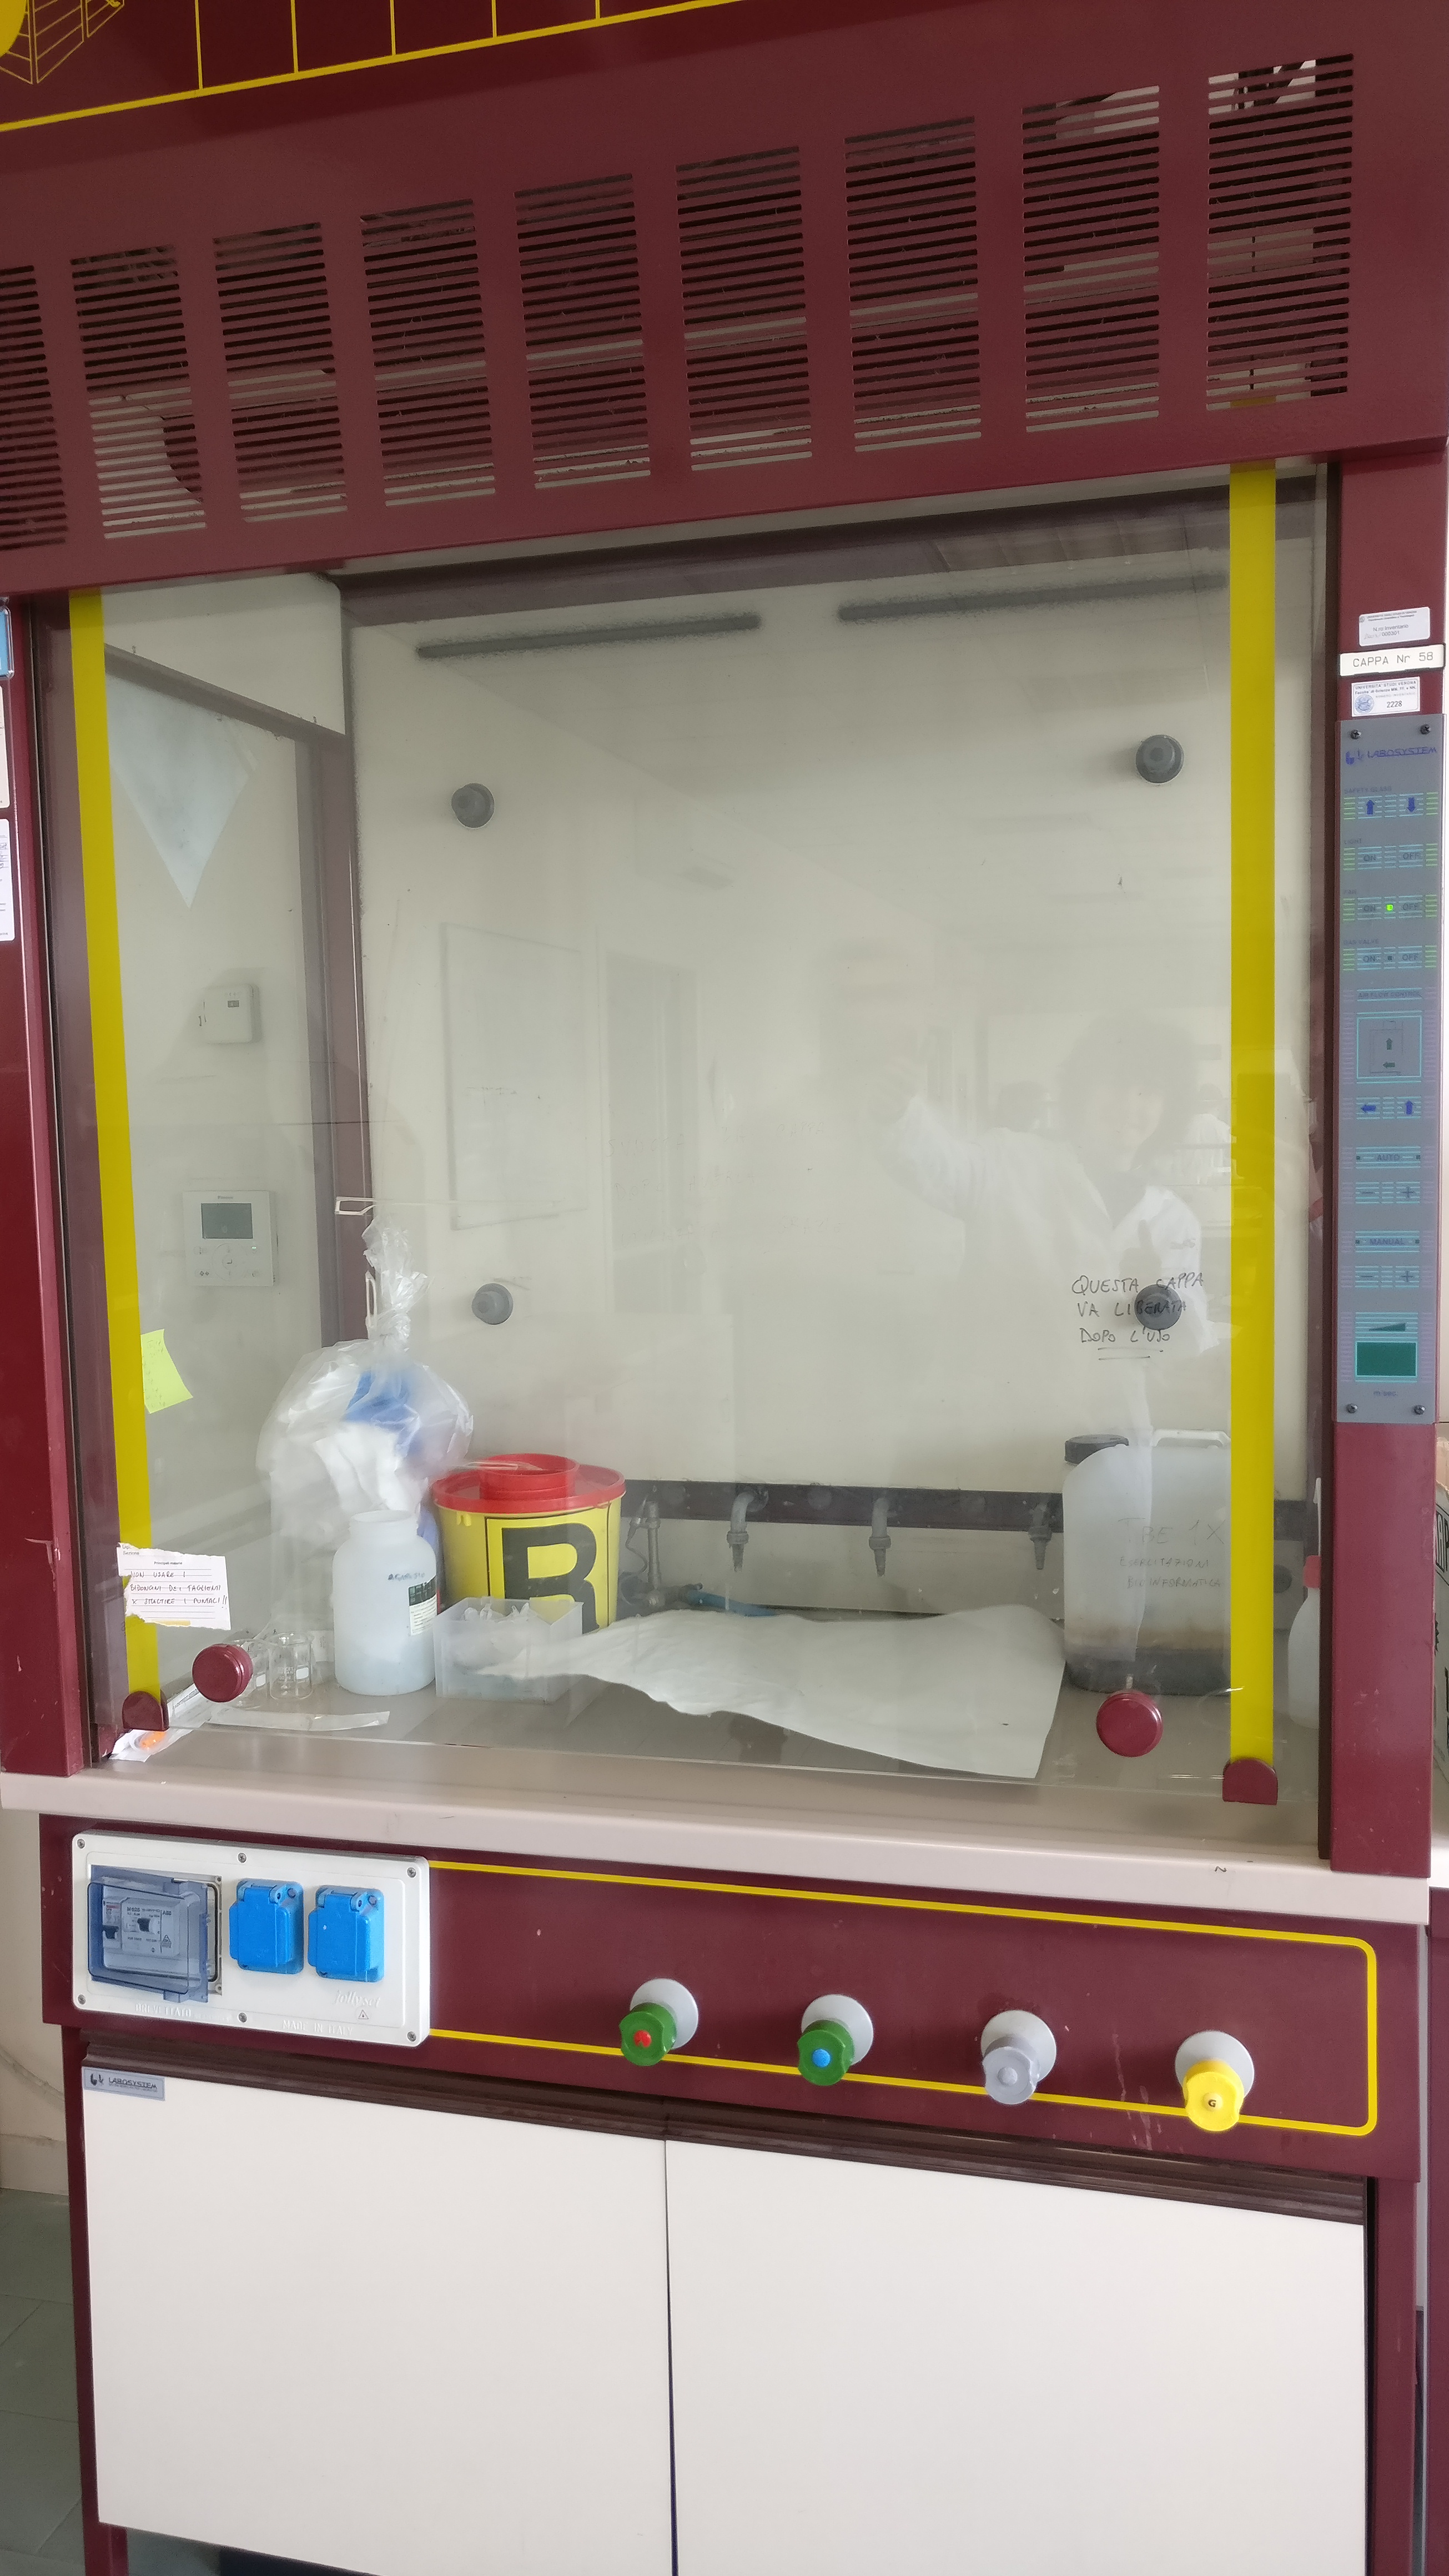
\includegraphics[width=0.4\textwidth]{./immagini/cappa_chimica.jpg}
			\caption{La cappa biologica o cappa aspirante, è un apparecchio utilizzato nei laboratori per proteggere l'operatore da eventuali vapori derivati da reazioni chimiche.}
			\label{cappa_chimica}

		\end{figure}

		\vspace{0.5cm}

Altri strumenti sono invece necessari in un laboratorio per poter \textbf{maneggiare accuratamente e nel modo più appropriato} i nostri materiali e le nostre sostanze. Questi materiali sono:
		\vspace{0.5cm}



		\item Provette Eppendorf :

		\begin{figure}[H]

			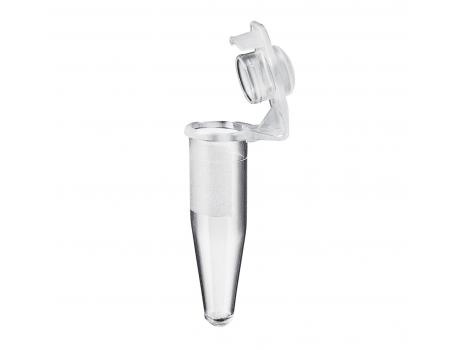
\includegraphics[width=0.6\textwidth]{./immagini/eppendorf.jpg}
			\caption{provetta Eppendorf, di dimensione variabile, da \SI{250}{\micro\liter} ai 2mL,
			utilizzate come provette monouso per piccole quantità di liquido. Utili nella centrifugazione.}
			\label{eppendorf}

		\end{figure}

		\vspace{0.5cm}


		\item Provette Falcon :

		\begin{figure}[H]

			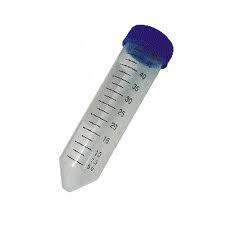
\includegraphics[width=0.5\textwidth]{./immagini/falcon.jpeg}
			\caption{la provetta falcon, così come quella eppendorf è un oggetto usa e getta, poichè non possono essere sterilizzate ad alte temperature,
			sono però abbasstanza resistenti alle basse temperature(per motivi di conservazione a ungo termine di campioni biologici). Anche queste
			possono contenere del materiale atto per le esperienze, sono più capacitive delle provette eppendorf.}
			\label{falcon}

		\end{figure}

		\vspace{0.5cm}


		\item Beuta:

		\begin{figure}[H]

			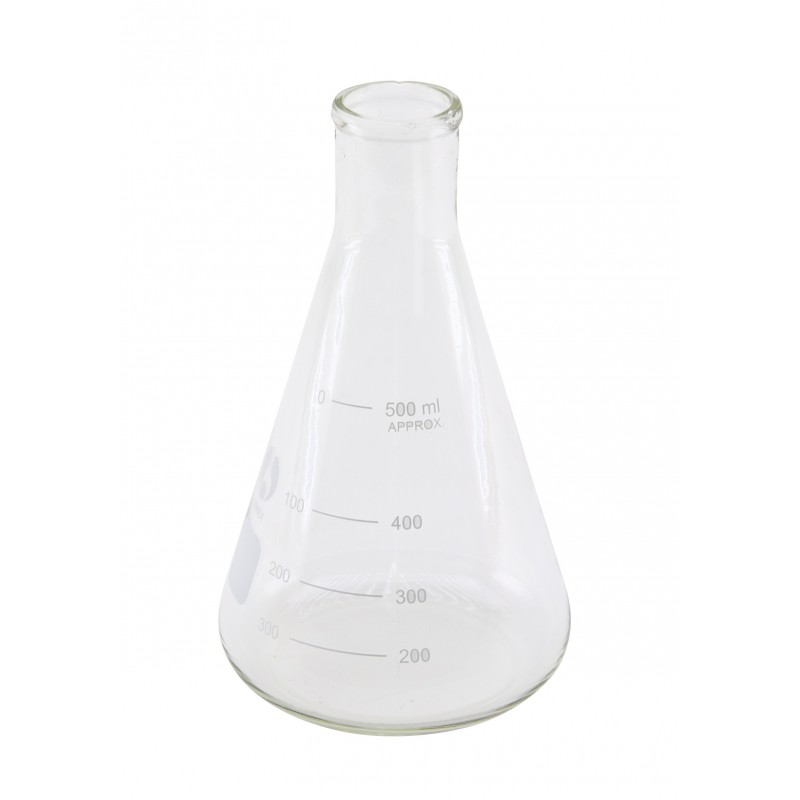
\includegraphics[width=0.5\textwidth]{./immagini/beuta.jpg}
			\caption{la beuta è un recipiente con base tronco-conica e collo cilindrica usato nei laboratori.
			Ne esistono di varie dimensione, solitamente vanno da una capacità di 10mL fino anche ad 1L.
			La forma particolare, ne consente la minimizzazione delle perdite di evaporazione e la possibilità
			di agitarne il contenuto senza spanderlo.}
			\label{beuta}

		\end{figure}

		\vspace{0.5cm}


		\item Bottiglia da laboratorio:

		\begin{figure}[H]

			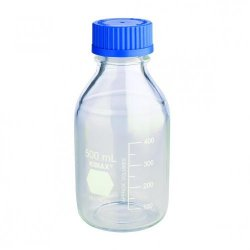
\includegraphics[width=0.5\textwidth]{./immagini/bottiglia.JPG}
			\caption{La bottiglia da laboratorio è un recipiente per le soluzioni che necessitano di un tappo per non far disperdere i gas durante le varie reazioni.}
			\label{bottiglia}

		\end{figure}

		\vspace{0.5cm}


		\item Piastra di Petri:

		\begin{figure}[H]

			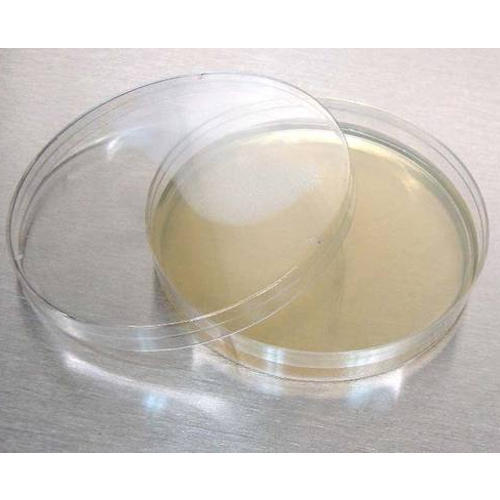
\includegraphics[width=0.5\textwidth]{./immagini/piastra_petri.jpg}
			\caption{La piastra di Petri o capsula di Petri è un recipiente di vetro o plastica,  solitamente a forma cilindrica; E' un apparecchio molto usato nei laboratorio di biologia, poichè su di esso si può far crescere culture cellulari. Le piastre hanno un diametri che varia tra 50 mm a i 100 mm ed un' altezza di 15 mm.}
			\label{piastra_petri}

		\end{figure}

		\vspace{0.5cm}


		\item pipette:

		\begin{figure}[H]

			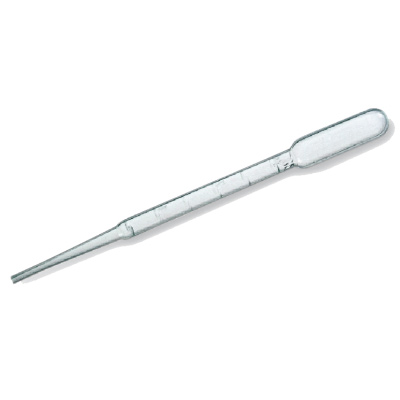
\includegraphics[width=0.5\textwidth]{./immagini/pipetta.jpg}
			\caption{La pipetta è uno strumento da laboratorio, con il uale si possoo prelevare determinate quantità di liquido. Sono poco precise nella misurazione delle quantità. per quello esistono le micropipette o le micropipette elettroniche.}
			\label{pipetta}

		\end{figure}

		\vspace{0.5cm}


		\item Micropipette e puntali:

		\begin{figure}[H]

			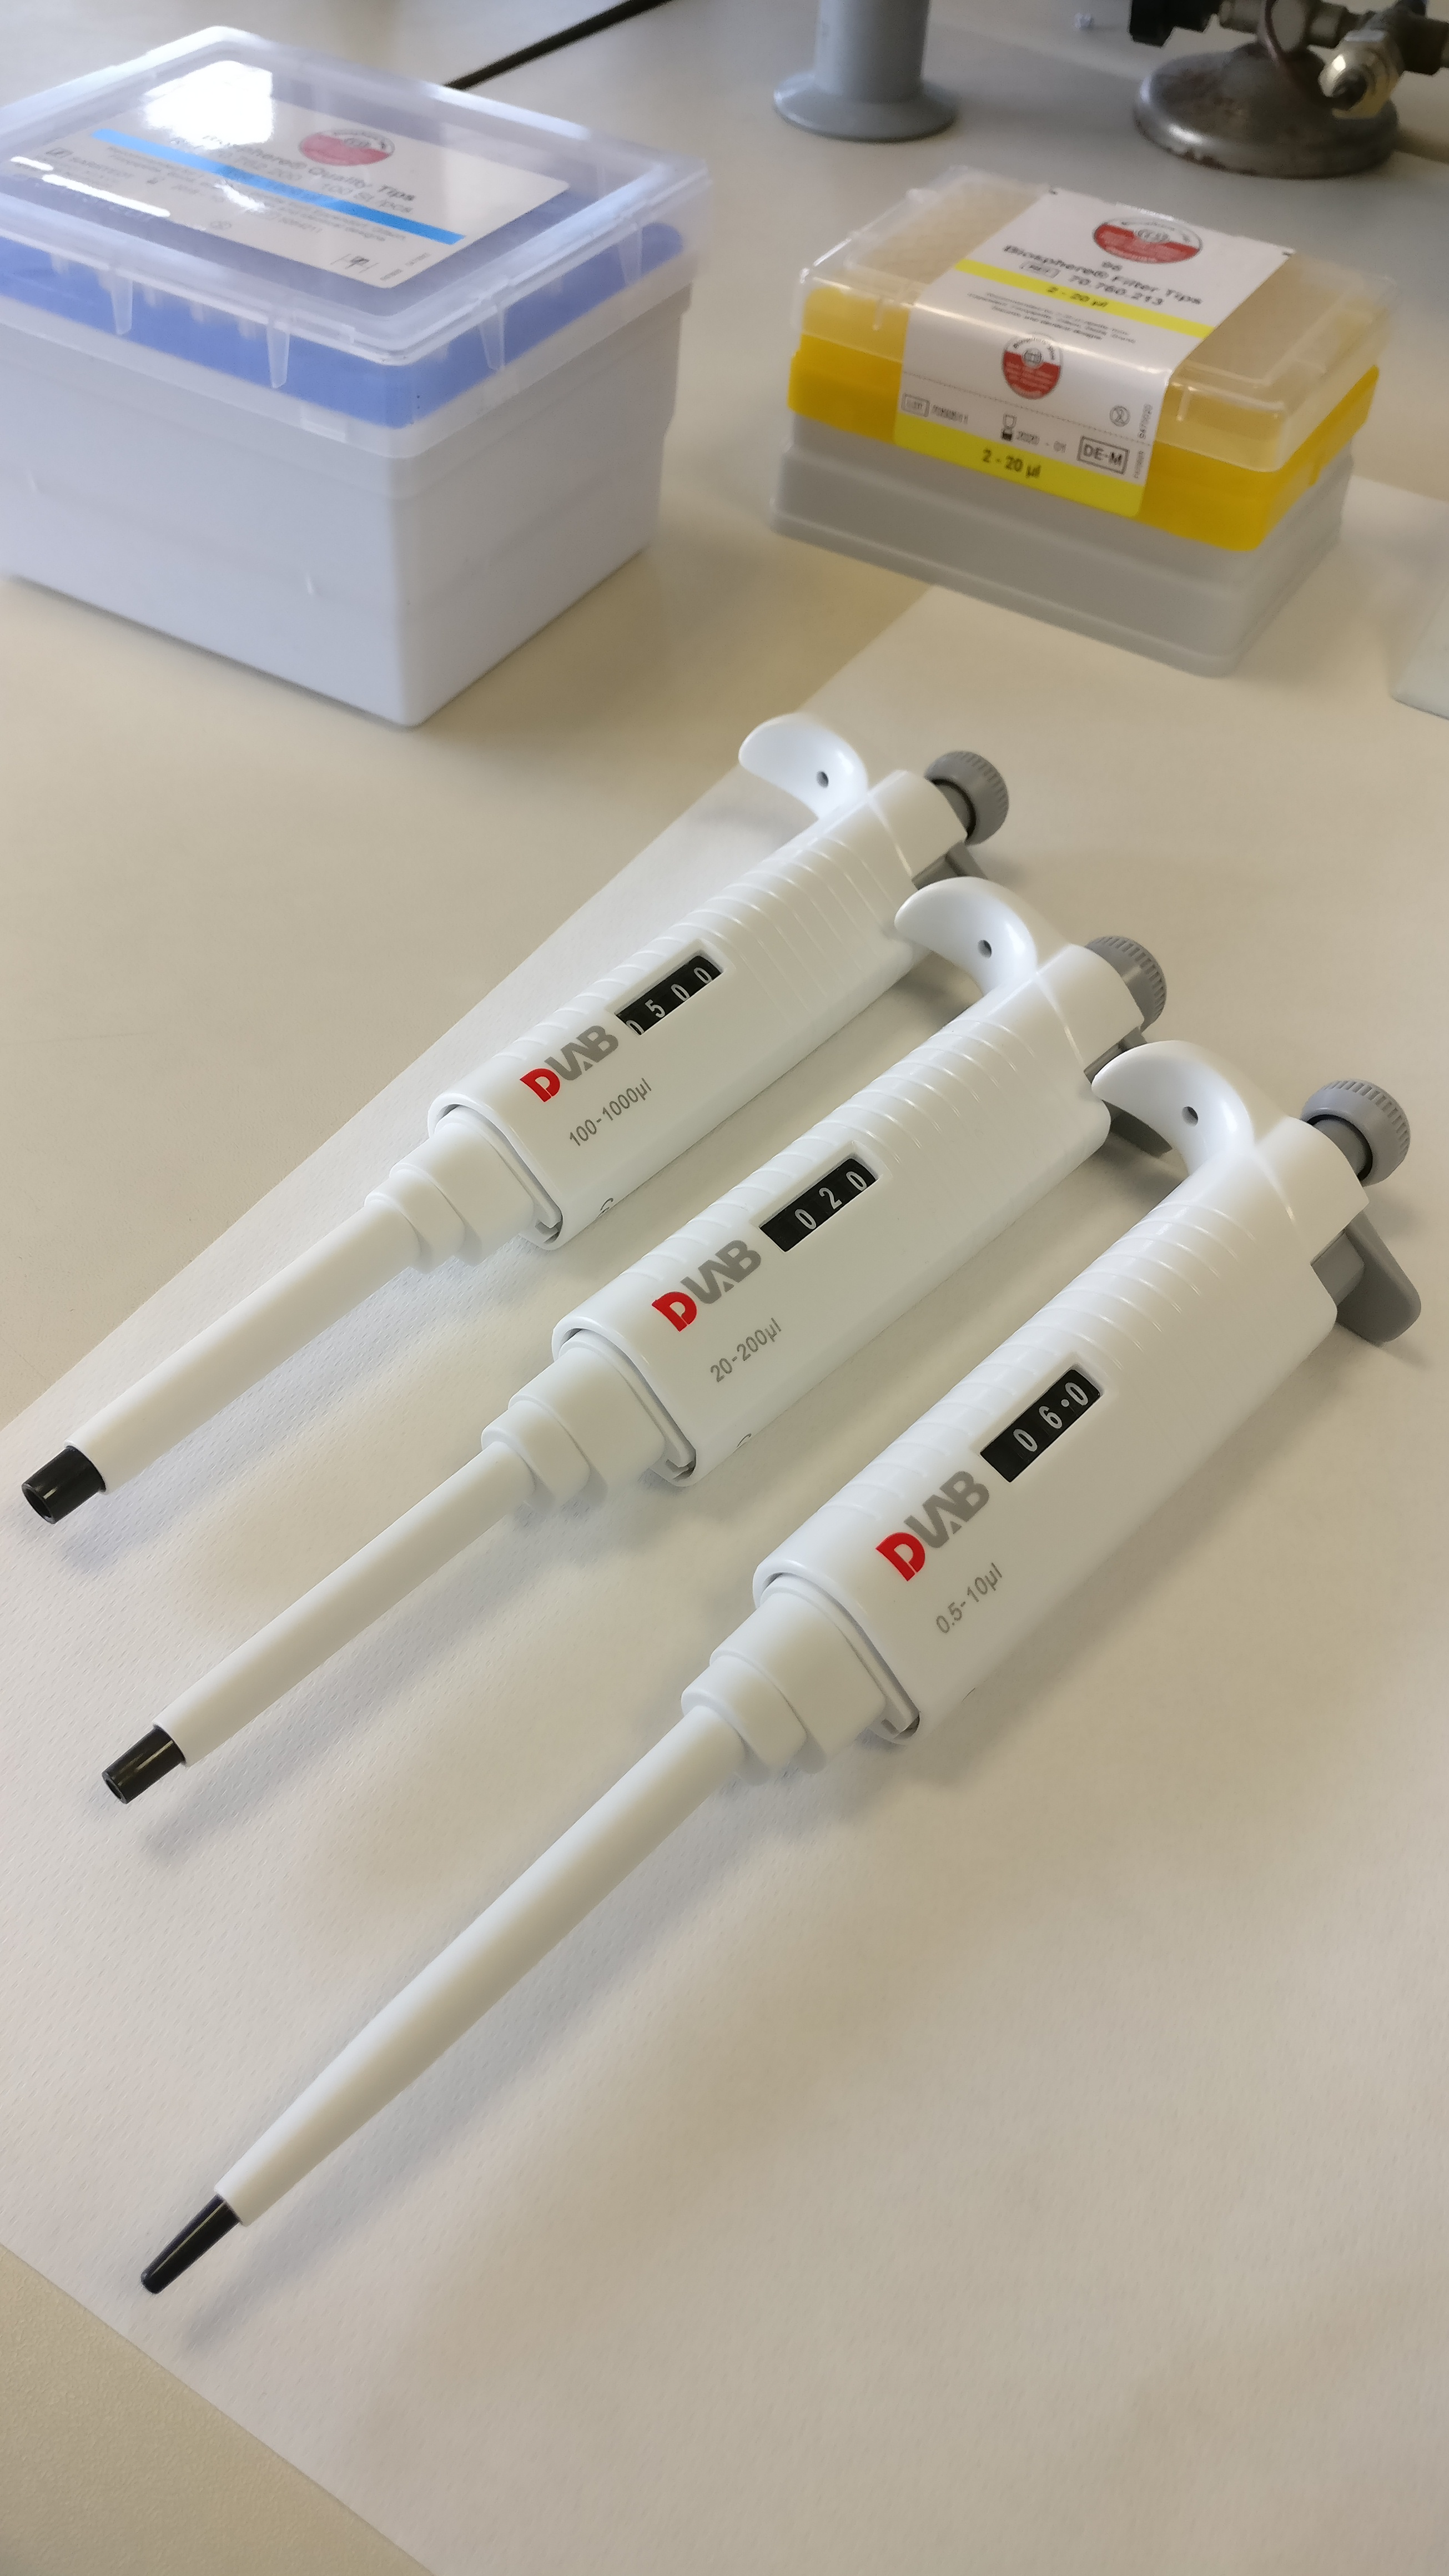
\includegraphics[width=0.35\textwidth]{./immagini/micropipette.jpg}
			\caption{Le micropipette ed i relativi puntali dietro, sono delle tipologie di pipette, però con la capacità precisiva più alta rispetto alle precedenti. Quelle usate in laboratorio da noi, consentono il prelievo di
			\SI{1000}{\micro\liter}-\SI{100}{\micro\liter}, \SI{200}{\micro\liter}-\SI{20}{\micro\liter},
			\SI{10}{\micro\liter}-\SI{0.5}{\micro\liter}. }
			\label{micropipette}

		\end{figure}

		\vspace{0.5cm}

		\textbf{Altri strumenti ancora}, sono invece necessari per poter andare ad \textbf{interagire} proprio con le nostre sostanze, facendogli compiere delle operazioni necessarie per raggiungere un risultato, come nel caso della vasca per l'elettroforesi necessaria per dividere le i nostri acidi nucleici o le nostre proteine in base alla loro carica, oppure il microscopio ottico, per andare a vedere la disposizione delle cellule nel nostro campione e poterle contare.
Questi strumenti sono:




		\item Microscopio ottico:

		\begin{figure}[H]

			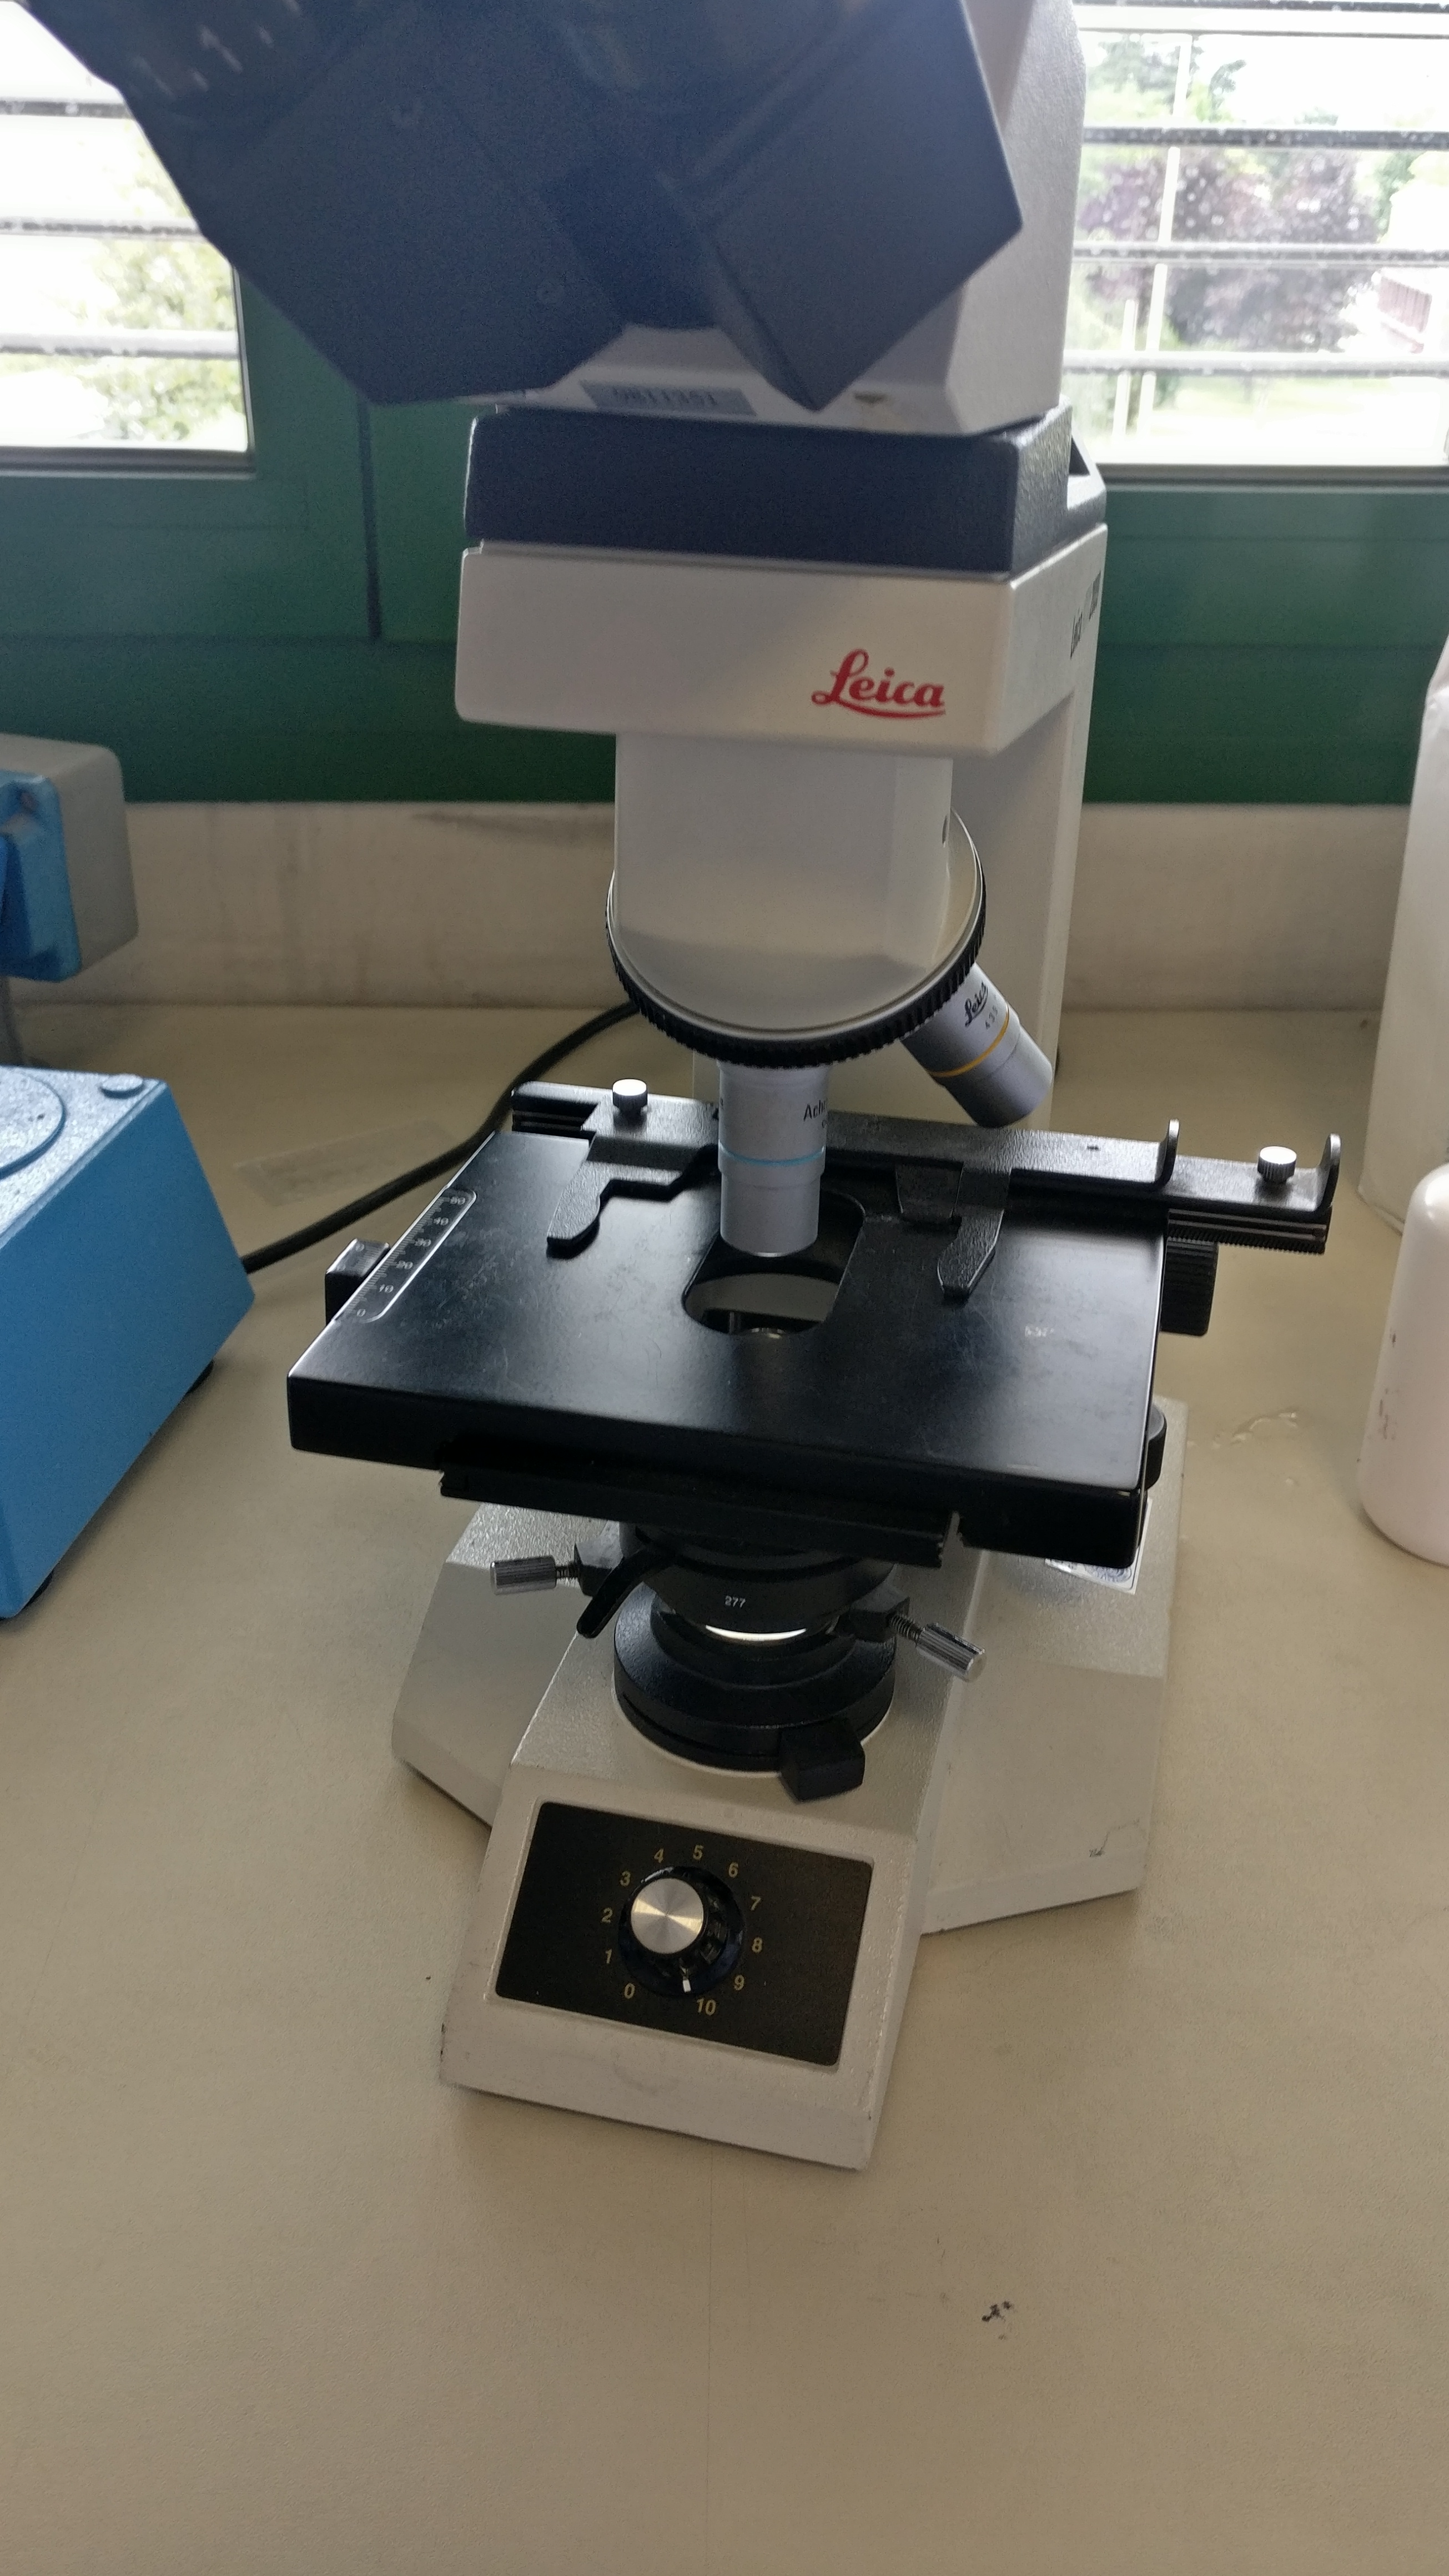
\includegraphics[width=0.35\textwidth]{./immagini/microscopio.jpg}
			\caption{Il microscopio ottico è un tipo di miscroscopio che sfrutta la luce con lunghezza d'onda dal
			vicino infraroso all'ultravioletto, coprendo tutto lo spettro visibile.
			E' il microscopio più semplice e antico della storia. Consente di ingrandire l'immagine di un campione
			illuminato con luce nell'intervallo spettrale del visibile,  per mezzo di lenti}
			\label{microscopio}

		\end{figure}

		\vspace{0.5cm}


		\item Vasca per l'elettroforesi:

		\begin{figure}[H]

			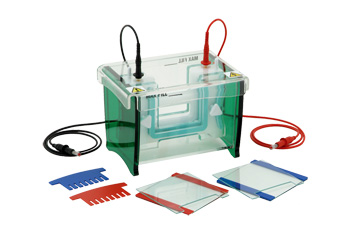
\includegraphics[width=0.6\textwidth]{./immagini/vasca_elettroforesi.jpg}
			\caption{Serve per l'appunto per l'elettroforesi, tecnca per analizzare e separare acidi nucleici, sfruttando cariche presenti nelle molecole di DNA e RNA per farle migrare.}
			\label{vasca_elettroforesi}

		\end{figure}

		\vspace{0.5cm}


		\item Centrifuga:

		\begin{figure}[H]

			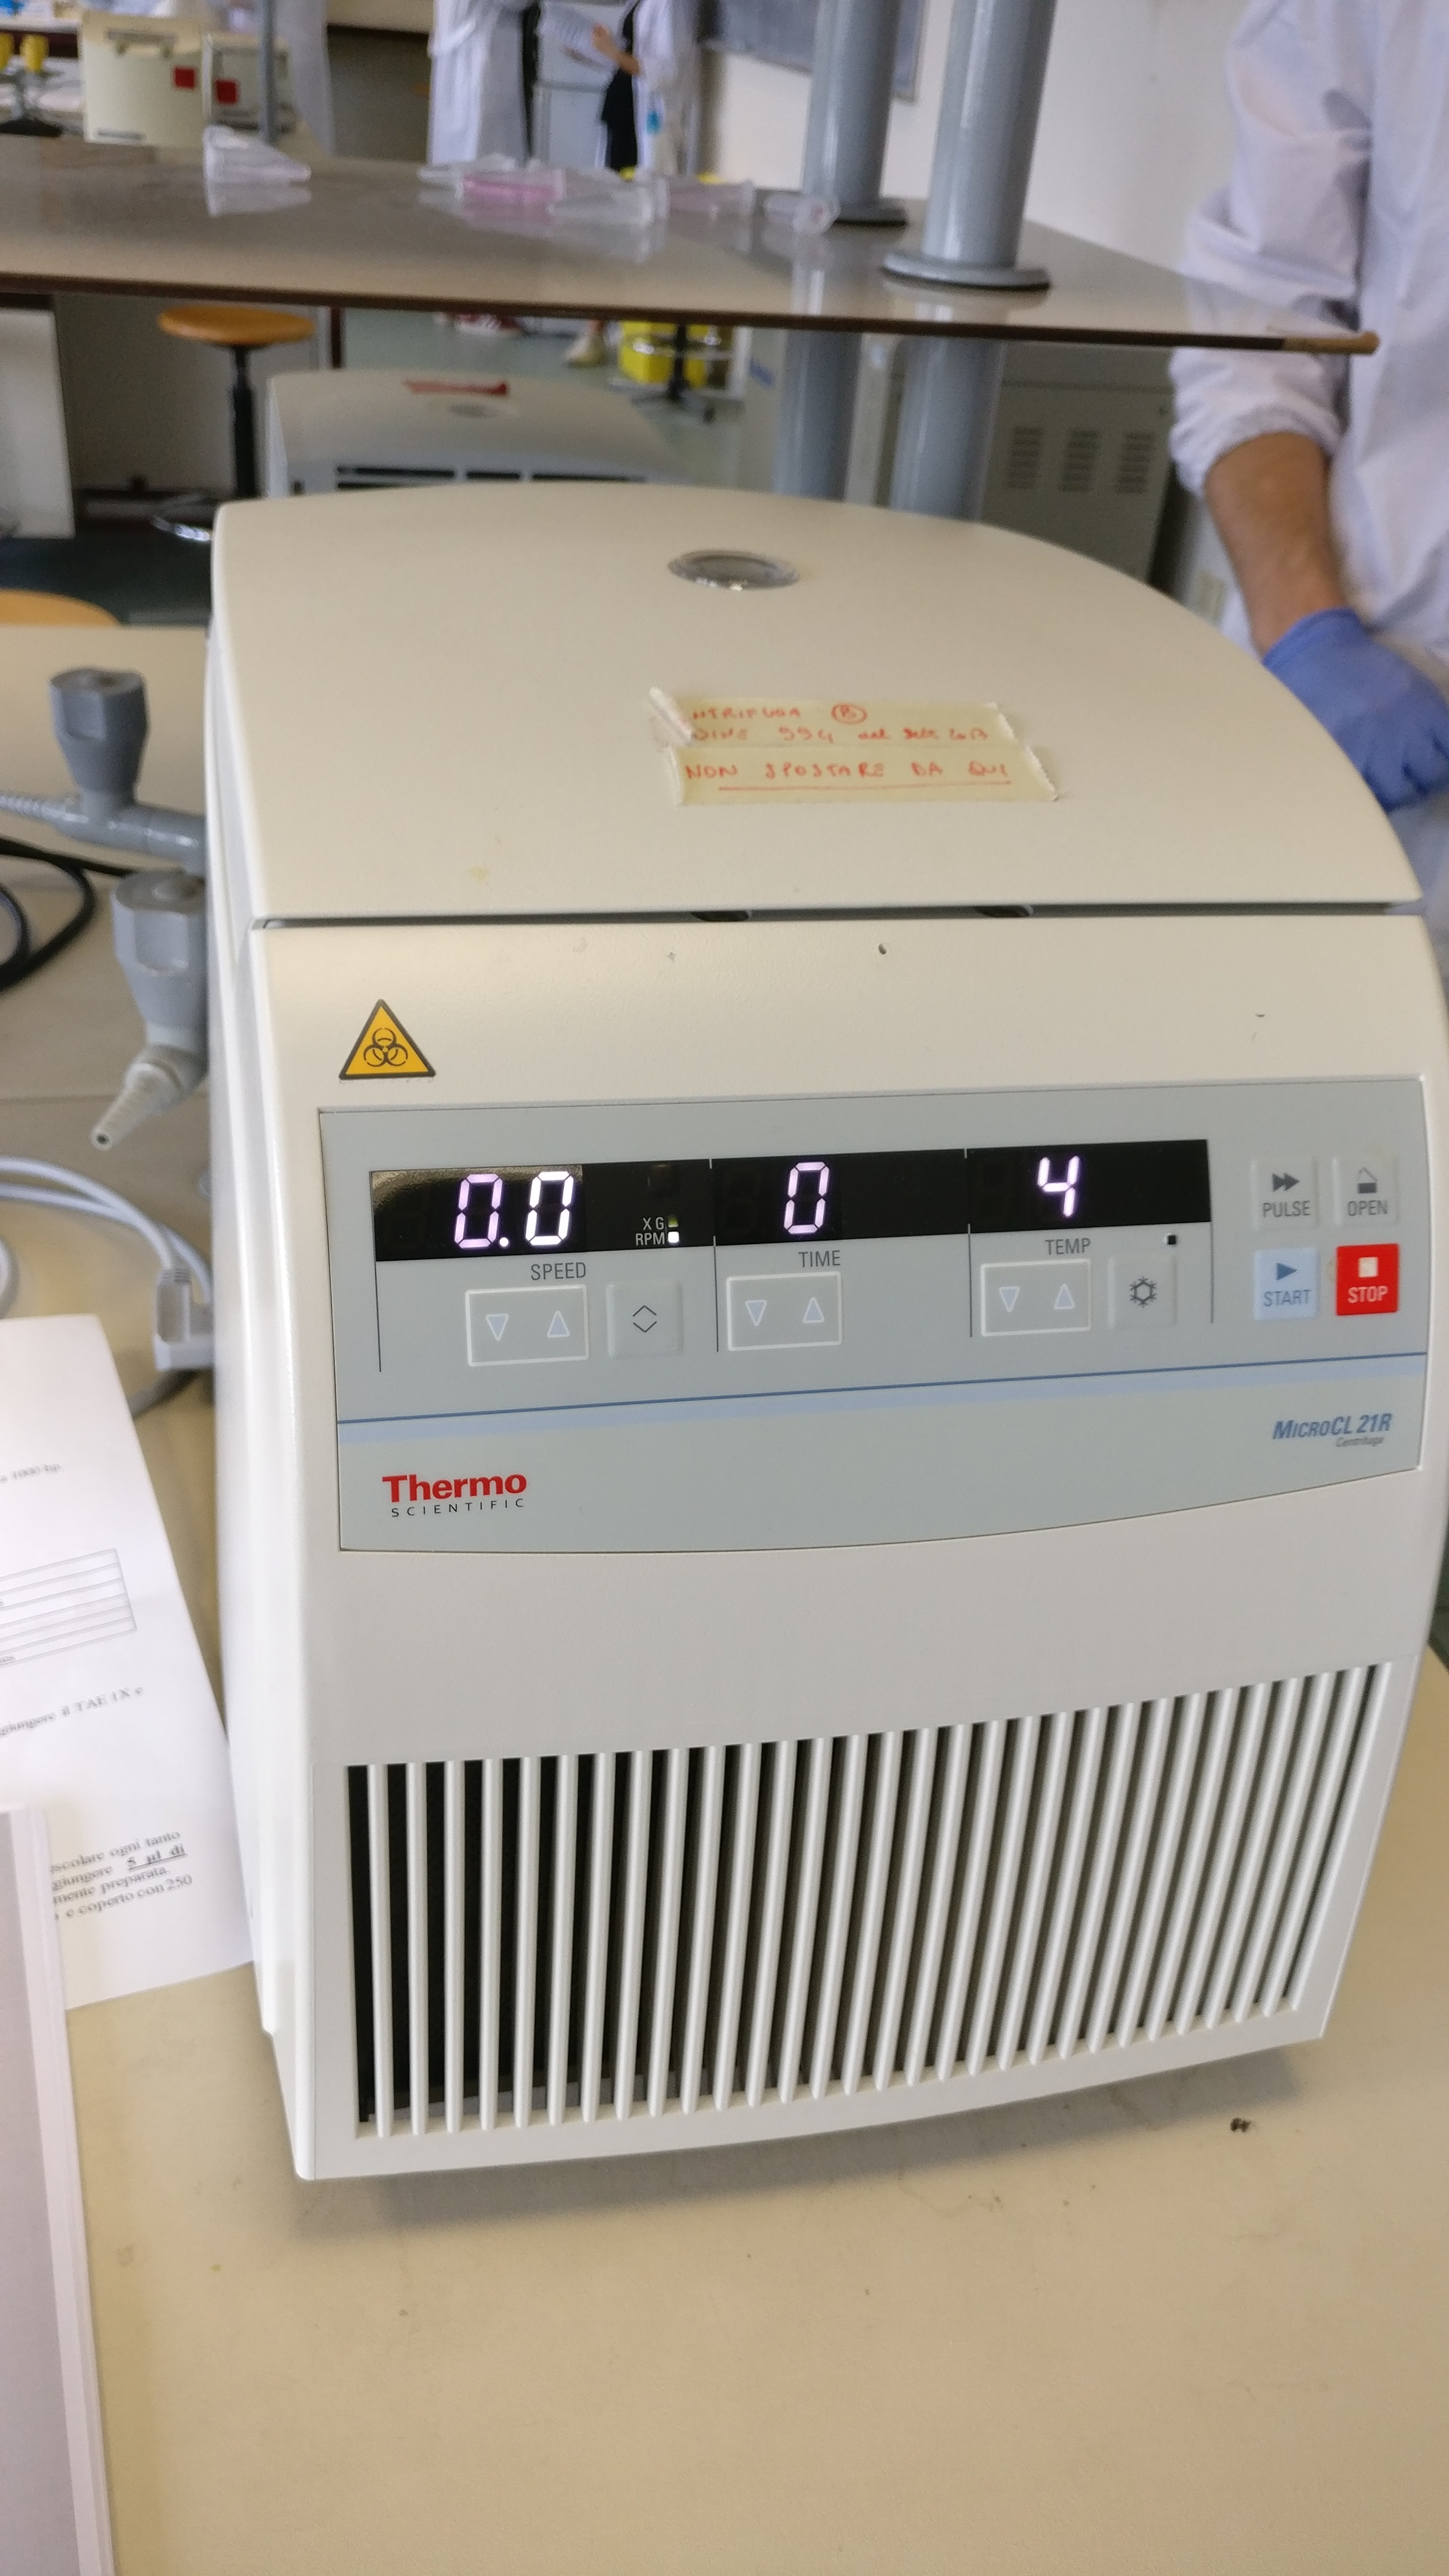
\includegraphics[width=0.35\textwidth]{./immagini/centrifuga.jpg}
			\caption{La centrifuga è un' apparecchiatura utilizzata nei laboratori per accellerare la separazione tra corpi aventi differente densità mediante l'uso della forza centrifuga.}
			\label{centrifuga}

		\end{figure}

		\vspace{0.5cm}


		\item Termociclatore:

		\begin{figure}[H]

			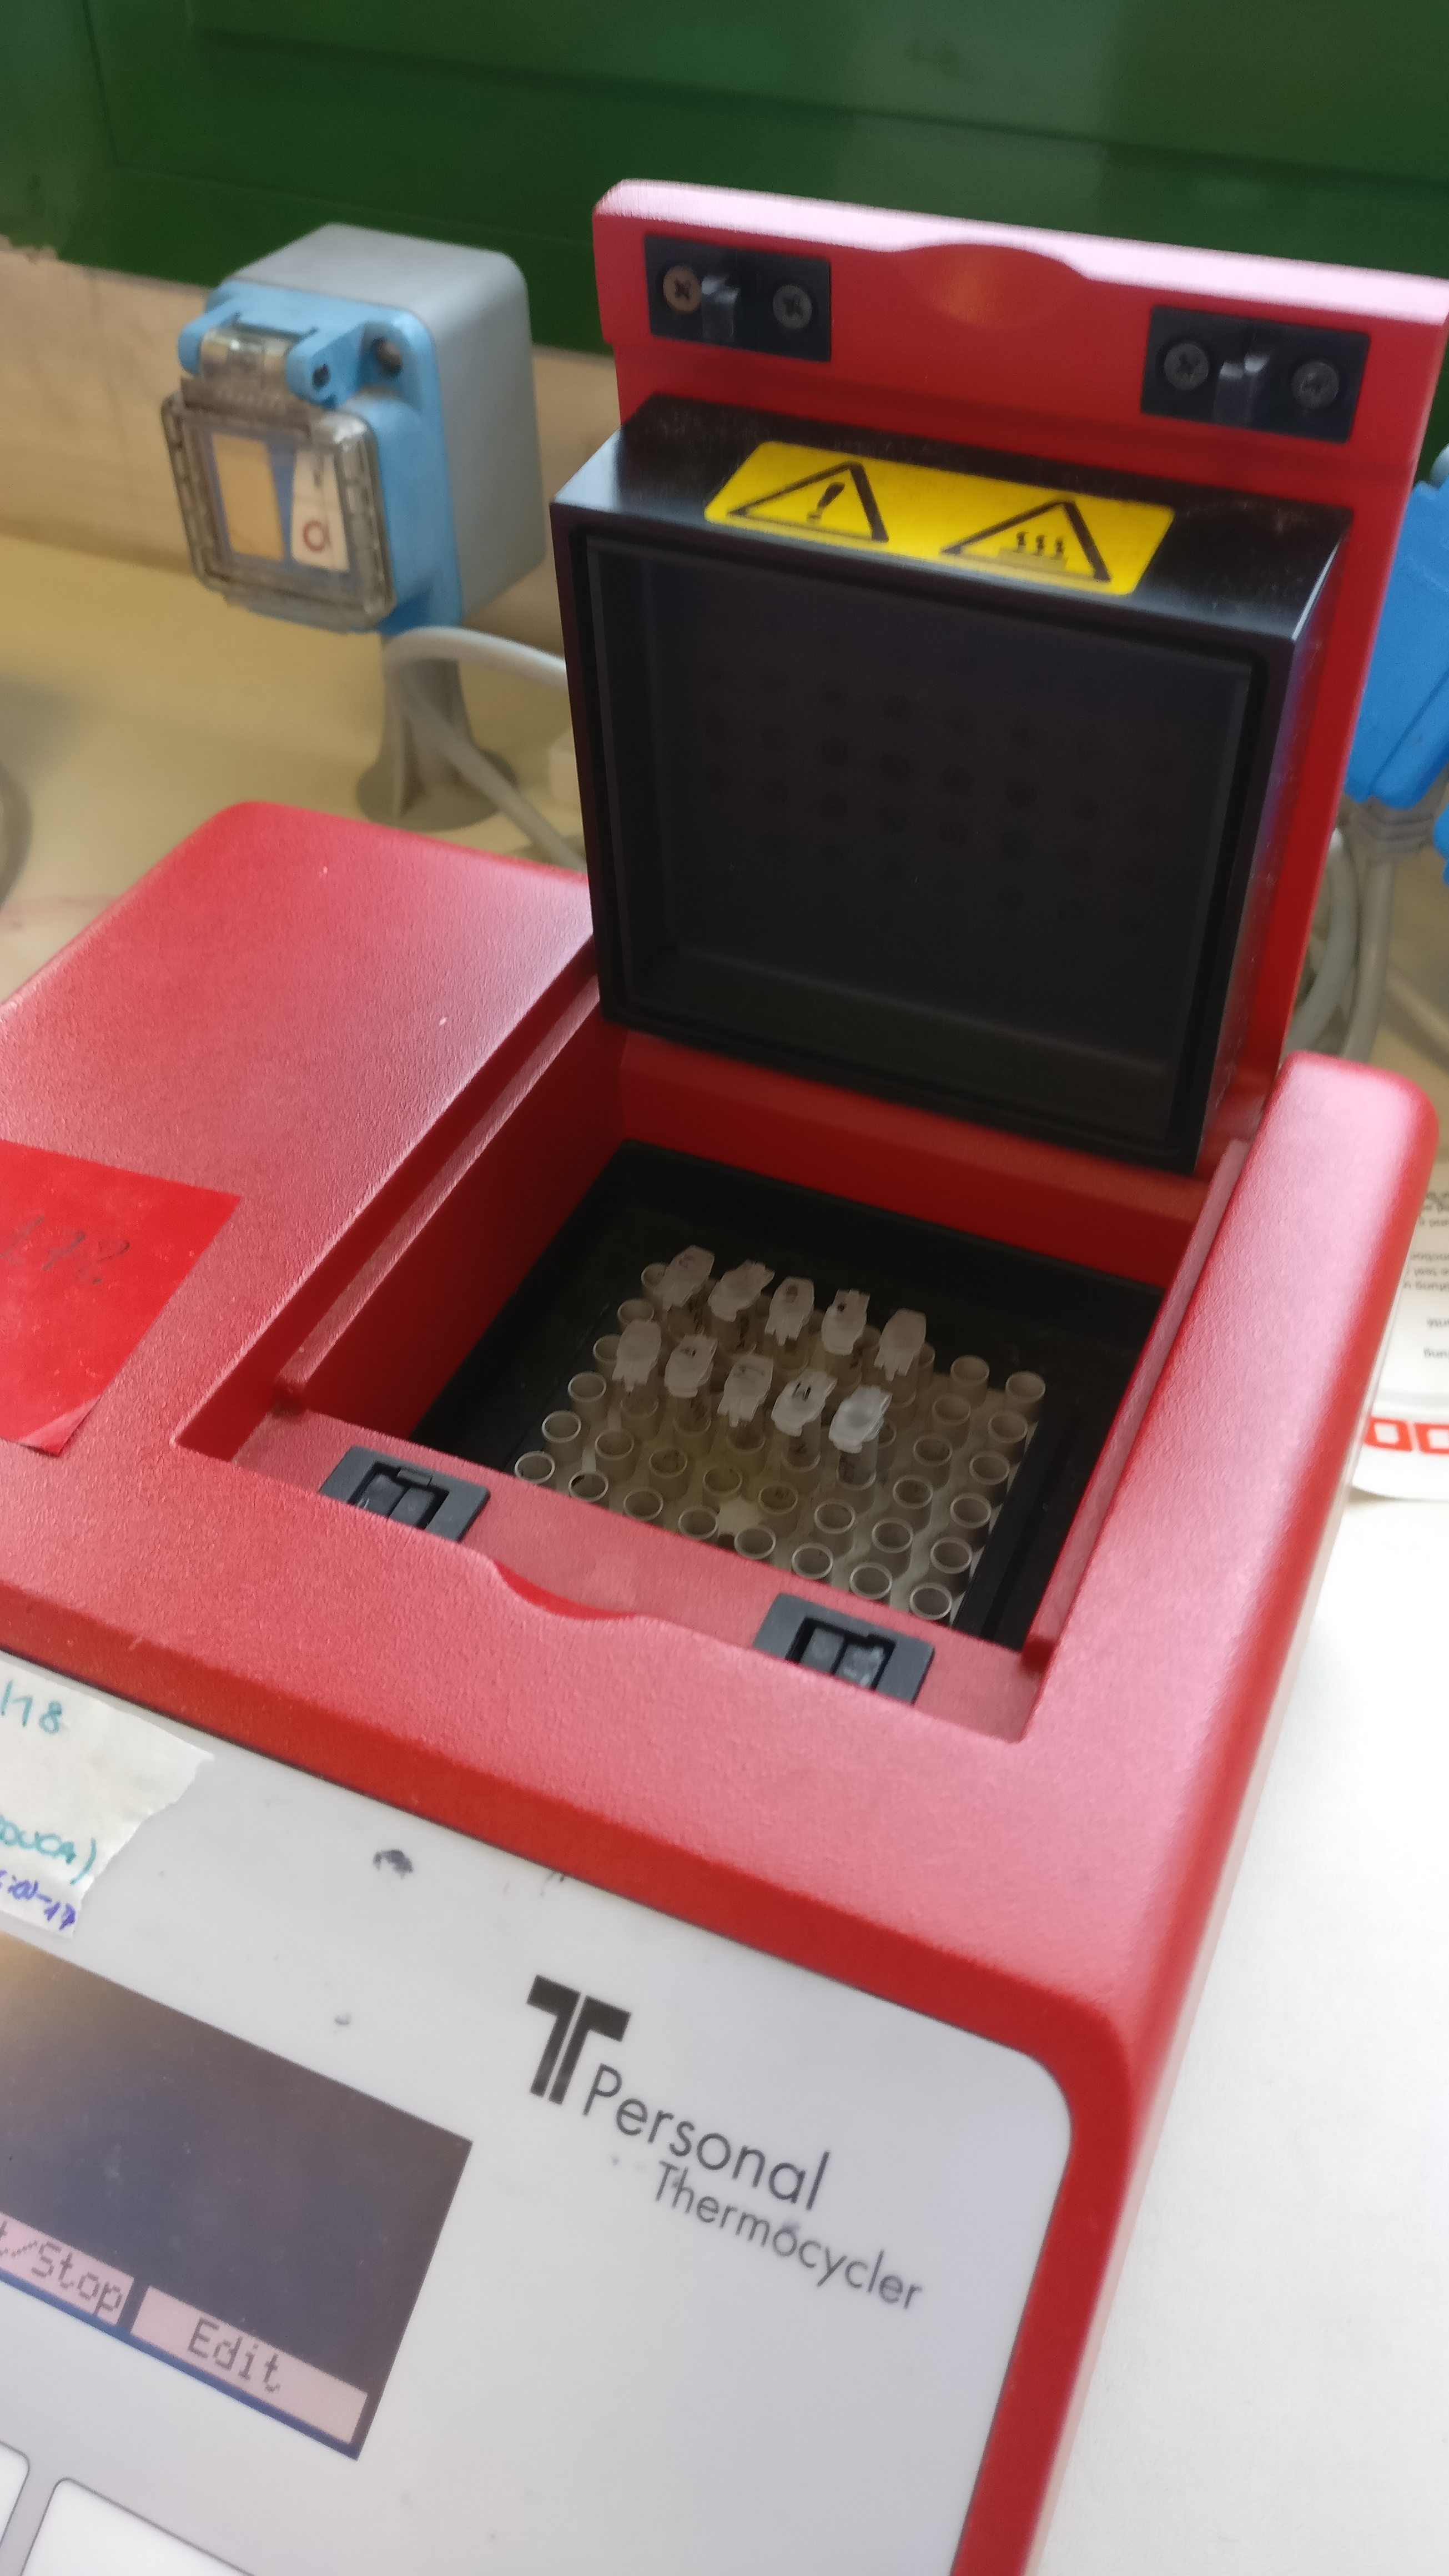
\includegraphics[width=0.35\textwidth]{./immagini/termociclatore.jpg}
			\caption{Il termociclatore è come dice la parola uno strumento che ad intervalli di tempo(cicli) fà variare la temperatura (termo). Questo strumento serve per l'amplificazione enzimatica di sequenze di DNA in vitro attraverso la reazione a catena della polimerasi (PCR).}
			\label{termociclatore}

		\end{figure}

		\vspace{0.5cm}


		\item Spettrofotometro:

		\begin{figure}[H]
			\centering

				\begin{subfigure}[b]{1\textwidth}

					\centering
			  	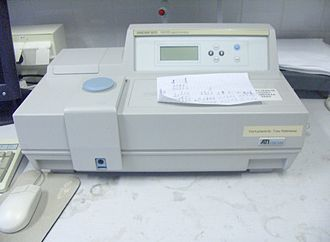
\includegraphics[width=0.35\textwidth]{./immagini/spettrofotometro.jpg}
					\caption{spettrofotometro a cuvetta}
					\label{spettrofotometro_cuvetta}

				\end{subfigure}

				\qquad

				\begin{subfigure}[b]{1\textwidth}
					\centering
					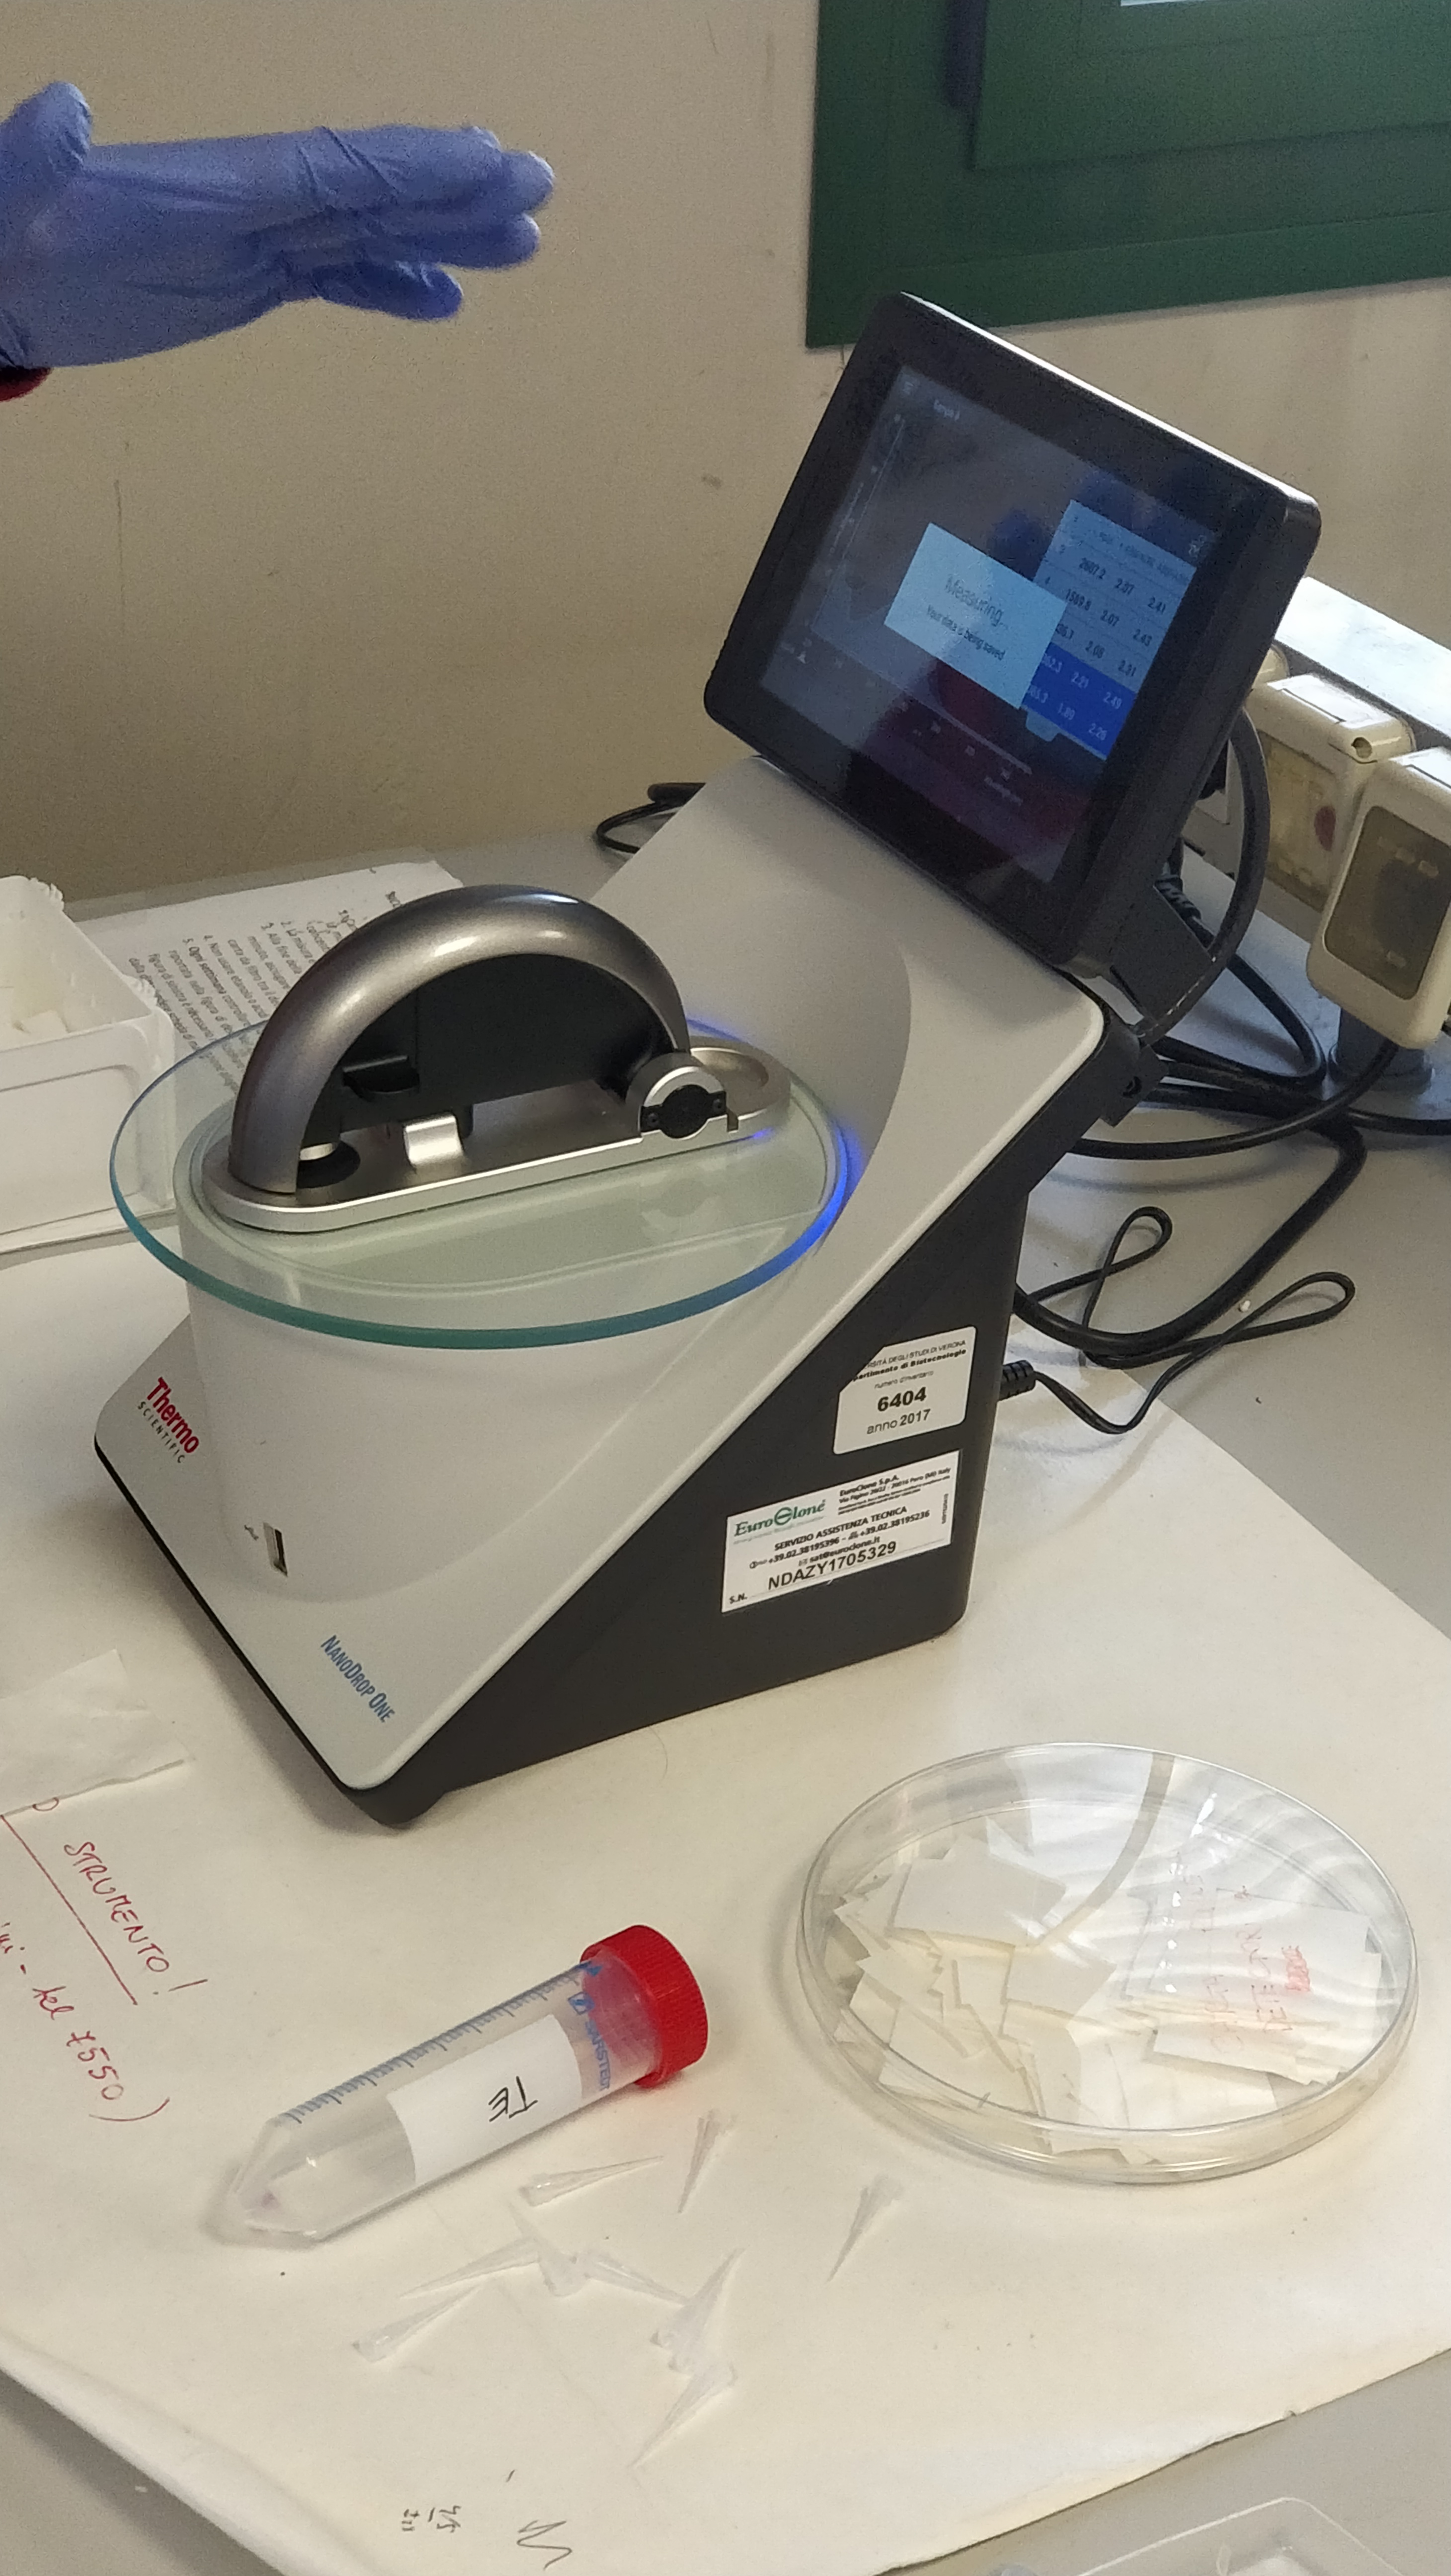
\includegraphics[width=0.35\textwidth]{./immagini/spettrofotometro_nanodrop.jpg}
					\caption{spettrofotometro nanodrop}
					\label{spettrofotometro_nanodrop}
				\end{subfigure}

				\quad

				\begin{subfigure}[b]{1\textwidth}

					\centering
			  	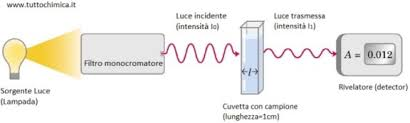
\includegraphics[width=0.35\textwidth]{./immagini/assorbanza.jpeg}
					\caption{Funzionamento dello spettrofotometro}
					\label{assorbanza}

				\end{subfigure}

			\caption{Lo spettrofotometro è uno strumento usato in laboratorio per la misura dell'intensità luminosa, che può determinare la misura dell'intensità come funzione della lunghezza d'onda.
			Grazie a questo possiamo sapere l'assorbanza della nostra miscela e quindi saperne la quantità e la purezza.}

		\end{figure}

		\vspace{0.5cm}




	\end{enumerate}


	\newpage

	\title{\huge{RELAZIONI:}}
	\maketitle
	\vspace{1.5cm}

	%_______________________________ESPERIENZA N° 1 (PREPARAZIONE DNA PLASMIDICO TRAMITE LISI ALCALINA)
	\section{\LARGE{Preparazione DNA plasmidico tramite lisi alcalina}}

\vspace{0.6cm}


\subsection{Sommario}

\subsubsection{Scopo}

L'obbiettivo di questa esperienza è quello di effettuare una miniprep, cioè una Minipreparazione di DNA plasmidico.
Dovremmo perciò andare tramite una lisi a rompere la membrana cellulare per estrarne il DNA plasmidico per poterlo utilizzare nele procedure di trasfezione.

\subsubsection{Cenni teorici}

La miniprep è una tecnica di laboratorio utilizzata per prelevare, in piccole quantità,
del DNA plasmidico dai batteri che lo contengono.

Innanzitutto andiamo a vedere nel dettaglio cos'è il DNA plasmidico.
I plasmidi sono piccoli filamenti circolari di DNA superavvolto a doppia elica, presenti nel citoplasma di tutti i batteri;
sono delle molecole estracromosomiali auto replicanti.
In natura i plasmidi assumono strutture diverse, grandezze diverse, numero di coppie diverse e modi di replicazione differenti in base al batterio che li contiene,
Questi plasmidi hanno l'abilità di propagarsi in batteri differenti, trasferirsi tra specie batteriche e forse la più importante sono i tratti genetici che trasportano.

\begin{figure}[H]

	\centering
	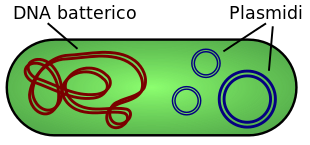
\includegraphics[width=0.6\textwidth]{./immagini/plasmide.png}
	\caption{illustrazione cellula batterica con DNA batterico (rosso) e DNA plasmidico (blu).}
	\label{plasmide}

\end{figure}

L'uso dei plasmidi è molto ingegnoso, in quanto permette di replicare il materiale genico all'interno dei batteri
oppure di trasferire certi geni in altri organismi.


\subsubsection{Materiali utilizzati}

\begin{itemize}
	\item Guanti in lattice
	\item Micropipette (\SI{100}{\micro\liter}-\SI{1000}{\micro\liter} e \SI{2}{\micro\liter}-\SI{200}{\micro\liter}  )
	\item Eppendorf (2ml)
\end{itemize}


\subsubsection{Soluzioni utilizate}

\begin{itemize}

	\item Soluzione I:
  \begin{enumerate}
    \item 50 mM glucosio
    \item 25 mM Tris-HCL (pH 8.0)
    \item 10 mM EDTA (pH 8.0)
  \end{enumerate}
	\item Soluzione II:
  \begin{enumerate}
    \item 0.2 NaOH
    \item 1 \% SDS
  \end{enumerate}
	\item Soluzione III:
  \begin{enumerate}
    \item 5M potassio acetato 60 mL
    \item acido acetico glaciale 11.5 mL
    \item acqua distillata 28.5 mL
  \end{enumerate}

\end{itemize}

\vspace{0.5cm}

\textbf{NOTE:}

\begin{itemize}
  \item La soluzione I è necessaria per risospendere le cellule e portarle in condizioni adatte per la successiva lisi;
  \item La soluzione II provoca la lisi alcalina delle cellule grazie a NaOH che denatura il DNA e l’SDS che è un detergente e denatura le proteine.
\end{itemize}

\subsection{Procedimento}

\subsubsection{Miniprep: }

\begin{enumerate}
  \item Prelevare 1.5 ml di coltura batterica fresca, in quanto l’utilizzo di colture vecchie potrebbe influenzare negativamente la corretta purificazione del DNA a causa dell’accumulo di metaboliti secondari. Non è rilevante la quantità di coltura batterica che si preleva ma tuttavia se ne prende in moda da riempire l’eppendorf per massimizzare la quantità di DNA. Non è indispensabile l’utilizzo di una cappa sterile: l’eventuale presenza di DNasi esogene viene contrastata con l’utilizzo, nelle fasi successive, di EDTA
  \item Centrifugare per 30’’ a 12000 rpm (non serve che centrifuga sia a 4° ma possimao centrifugare direttamente a temperatura ambiente) consentire la formazione di un pellet più o meno compatto(quelli riportati sono valori di centrifugazione indicativi: se il pellet è instabile procedere con un’ulteriore centrifugazione). Finita la centrifuga eliminare il surnatante versando il contenuto del tubo e pichiettare leggermente con il tappo aperto, cercando di allontanare il più possibile eventuali gocce dal terreno, per non modificare le concentrazioni delle tre soluzioni che verranno usate in seguito.

  \item Risospendere il pellet batterico in 100 μl di Soluzione I. Per la risospensione si può utilizzare il vortex o il puntale di una pipetta, in quanto le cellule sono ancora integre ed il DNA è protetto.

  \item Aggiungere 200 μl di Soluzione II e mescolare. Essendo una soluzione alcalina, provoca la lisi delle cellule, la denaturazione e la  precipitazione delle molecole di DNA genomico e plasmidico.
Le molecole di DNA a causa della lisi diventano estremamente fragili, per questo si deve mescolare adeguatamente ma evitando azioni troppo energiche (vortex) per non rompere il DNA stesso.
Come risultato si ottiene un lisato cellulare viscoso e biancastro.

  \item Aggiungere 150 μl di soluzione III entro 2-3 minuti dall’aggiunta della Soluzione II e mescolare capovolgendo il tubo due o tre volte in maniera delicata(non vortexare). Aggiungendo la soluzione III si riporta il lisato cellulare a pH che permette la rinaturazione del DNA plasmidico.
La tempistica che precede l’aggiunta della soluzione III è fondamentale per la separazione del DNA plasmidico dal genomico: il DNA plasmidico, proprio perché superavvolto e di piccole dimensioni, se mantenuto in condizioni di lisi per un tempo non superiore ai 3-4 minuti riesce a rinaturare, mentre il DNA genomico e le proteine rimangono intrappolate irreversibilmente nel complesso formato da potassio e SDS. Nel caso la soluzione II venisse lasciata agire per periodi più lunghi, il DNA plasmidico sarebbe comunque in grado di rinaturare ma assumerebbe una conformazione tale da risultare inattaccabile dagli enzimi di restrizione.

  \item Centrifugare a massima velocità per 5 minuti per permettere la sedimentazione dei residui cellulari e recuperare il surnatante in un nuovo tubo. E’ consigliato prelevare una quantità non superiore a 550μl. Questo perché verrà aggiunto un volume doppio di etanolo nelle fasi successive.

  \item OPZIONALE : Trattamento con fenolo-cloroformio per eliminare le proteine rimanenti. Questo trattamento verrà spiegato singolarmente più avanti.

  \item Precipitare il DNA con due vol. di etanolo (100\% v/v) oppure con 0.6 vol. di isopropanolo. L'etanolo è aggiunto al 100\% per ottenere una soluzione finale al 70\%. Per esempio: a 100 μl di DNA si aggiungono 200 μl di etanolo assoluto oppure 60 μl di isopropanolo. In questa fase è necessario capovolgere il tubo delicatamente, infatti il DNA deve venire a contatto con l’alcol per precipitare.

  \item Centrifugare a 12000 g per 5 minuti. Se il DNA è sporco è possibile vedere il pellet bianco sul fondo del tubo. Invece in presenza di una grande quantità di polisaccaridi il pellet è mucillaginoso.

  \item Rimuovere il supernatante e lavare con etanolo 70\% v/v, che permette di eliminare i sali rimasti. Per eliminare l’etanolo effettuare un breve passaggio in centrifuga (30” a massima velocità) per far scendere eventuali goccioline sul fondo del tubo e quindi aspirarle con una micropipetta, oppure capovolgere la provetta e scuoterla leggermente sulla carta. Versare nel tubo circa 500 μl di EtOH 70\%.

  \item Rimuovere completamente l’etanolo aspirandolo con una micropipetta senza rompere il pellet e lasciarlo asciugare all’aria per 10 minuti. L’asciugatura può essere velocizzata ponendo la provetta in un luogo ben aerato, come ad esempio una cappa a flusso laminare. E’ importante che il pellet sia completamente asciutto perché la presenza di tracce di etanolo determina una scarsa risospensione del DNA e, soprattutto, ne provoca la fuoriuscita dal pozzetto quando si effettua il caricamento su gel di agarosio per un’elettroforesi.

  \item Risospendere il DNA plasmidico in 50 μl di TE pH 8.0 che permette la risospensione evitando la degradazione. Infatti, il TE è composto da EDTA che garantisce protezione dalle DNAsi.

  \item Conservare a 4°C. Mentre, se si risospende in acqua si deve conservare a –20°C.

\end{enumerate}

\subsubsection{Trattamento con Fenolo-cloroformio}

Il fenolo cloroformio è una soluzione sinergica altamente deproteinizzante che serve per eliminare i possibili contaminanti del DNA(esempio: elimina proteine in sospensione in eccesso) per evitare che interferiscano con i successivi trattamenti, specialmente nel caso in cui si lavori con enzimi di restrizione. Questo trattamento può essere fatto anche su DNA genomico o comunque su DNA plasmidico già risospeso in TE. Il passaggio in fenolo:cloroformio deve sempre esser seguito da precipitazione in etanolo assoluto (o isopropanolo) e successiva risolubilizzazione in TE.

\begin{enumerate}
  \item Aggiungere alla soluzione contenente il DNA 1 vol. di fenolo:cloroformio:isoamilico (25:24:1)
La presenza dell’isoamilico serve per semisaturare il cloroformio che altrimenti puro avrebbe la tendenza a disidratare il campione.

  \item Miscelare le due fasi (non vortexare) fintanto che il campione non si presenta lattiginoso.

  \item Centrifugare almeno 3 minuti e in tal modo si formano due fasi distinte. Una fase inferiore di fenolo-cloroformio e una superiore con il DNA in soluzione. L’interfaccia bianca è data dalle proteine denaturate.

  \item Recuperare la fase superiore, contenente il DNA, facendo attenzione a non prelevare anche la fase inferiore. Tenere la punta della pipetta appena sotto la superficie dello strato superiore (Fig.1). Ad un certo punto si forma una bolla di soluzione contenente il DNA. E’ consigliato tenere inclinato il tubo in modo da prevedere dove si formerà la bolla(Fig.2) contente il DNA in moda tale da prelevarne la maggior quantità possibile. Bisogna assolutamente evitare di trasportare il fenolo-cloroformio perché queste degraderebbero gli enzimi utilizzati in seguito.

  \item Precipitare il DNA con etanolo o isopropanolo. Se inizialmente il DNA era in TE, è necessario aggiungere 1/10 vol. NaOAc 3M pH 4.8 prima di aggiungere i 2 vol. di etanolo assoluto oppure gli 0.6 vol. isopropanolo. Qualora questo trattamento venga condotto durante la Miniprep (punto 5), la presenza massiccia di sali forniti con la Sol. III  rende inutile (se non dannosa) l’aggiunta di 1/10 vol. NaOAc 3M pH 4.8 prima dell’alcool. In questo caso la precipitazione deve essere condotta come da punto 6 del protocollo Miniprep.


\end{enumerate}

\subsection{Risultati e Conclusioni}

Come conclusione di questa esperienza, possiamo dire di aver capito come estrarre dei frammenti di DNA (plasmidi) dalle cellule batteriche di E.coli tramite questa lunga procedura e nella prossima relaizone spiegheremo a cosa questi plasmidi verranno usati.

	\newpage

	%_______________________________ESPERIENZA N° 2 (Estrazione e quantificazione RNA totale)
	\section{\LARGE{Estrazione dell’RNA totale con TRIZOL}}

\vspace{0.6cm}


\subsection{Sommario}


\subsubsection{Scopo}
In questa esperienza vediamo l’estrazione dell’acido ribonucleico da tessuto vegetale per quantificarlo assieme al DNA. Oggi questa procedura si puo’ effettuare con diversi protocolli molto efficienti che anche partendo da piccole quantita’ di materia prima riescono a dare risultati.

\subsubsection{Cenni teorici}

\subsubsection{Materiali utilizzati}

\begin{itemize}
\item Eppendorf da 2ml
\item Micropipette assortite
\item Centrifuga
\end{itemize}

\subsubsection{Soluzioni utilizzate}
\begin{itemize}
\item Azoto liquido
\item TRIZOL
\item Cloroformio
\item 2-propanolo
\item Etanolo
\item Acqua DEPC
\end{itemize}

\subsection{Procedura}

\subsubsection{Estrazione dell'RNA totale}

\begin{enumerate}
\item Triturare le foglie in un mortaio aggiungendo azoto liquido per favorire la polverizzazione del tessuto vegetale delle foglie usate come campione. Avendo una polvere fina e’ possibile rompere le pareti cellulari. Prendere 100mg di polvere e trasferirli all’interno di una eppendorf da 2ml.

\item Risospendere i tessuti triturati in TRIZOL (1ml per 50/100mg di tessuto) e vortexare per 10s. Si usa TRIZOL per distruggere i componenti cellulari, denaturare le proteine ma lasciare intatto l’RNA.

\item Per assicurarsi che il TRIZOL agisca in modo efficace e che si abbia una completa dissociazione dei complessi nucleoproteici, lasciare il campione per 5 minuti a temperatura ambiente.

\item Aggiungere per ogni ml di TRIZOL 0.2 ml di cloroformio, vortexare vigorosamente per 15 secondi. Con il cloroformio minimizziamo le probabilità di contaminazione e stabilizziamo le 3 fasi che si formeranno in seguito.

\item Lasciare 15’ a temperatura ambiente.

\item Centrifugare per 15’ a 4°C e 1200 g. Grazie alla centrifugazione si ottengono 3 diverse fasi all’interno della eppendorf:
	\begin{itemize}
	\item Una fase organica di colore rosso contenente le proteine.
	\item Una interfase contentente il DNA genomico precipitato	.
	\item Una fase acquosa superiore contenente RNA.
	\end{itemize}

\item In una nuova provetta trasferire la fase acquosa, aggiungere 0.5ml di 2-propanolo per ml di TRIZOL usati e mescolare. Grazie al 2-propanolo si ottiene un lavaggio grazie alla diversa carica dei sali rispetto ai materiali organici.

\item Lasciare 20 minuti a -20°C e successivamente centrifugare nuovamente a 1200 g a 4°C. Con questa centrifuga, sul fondo della provetta si formerà del pellet composto dall’RNA.

\item Rimuovere il surnatante e aggiungere 1ml di etanolo per ogni ml di TRIZOL usato in modo da lavare il pellet.

\item Vortexare il campione e centrifugarlo nuovamente a 1200 g a 4°C per 5 minuti.

\item Asciugare il pellet per 10 minuti all’aria ma facendo attenzione che non si secchi completamente. Per asciugarlo possiamo lasciare la provetta aperta e leggermente inclinata verso il basso.

\item Aggiungere un volume (\SI{50/100}{\micro\liter}) di acqua DEPC e risospendere.
\end{enumerate}

\subsubsection{Quantificazione dell’RNA totale e del DNA tramite spettroscopia UV}

\textbf{Spettrofotometro a Cuvetta}
\vspace{0.5cm}

\begin{enumerate}
\item  Diluire 1:20 il campione di RNA in acqua DEPC, ottenendo un volume finale di 500ml in una eppendorf.
\item  Registrare il bianco con una eppendorf contentente solo acqua DEPC e aquisire lo spettro di assorbimento tra \SI{230/400}{\nano\meter}.
\item  Calcolare la quantità di RNA contenuta e la sua purezza tenendo conto delle diluizioni. La purezza è indicata con il rapporto tra A260/A280.
\end{enumerate}

\textbf{Spettrofotometro NanoDrop}
\vspace{0.5cm}
Si misura la concentrazione di pUC18 (riferimento alla prima esperienza)
\begin{enumerate}
\item Depositare una goccia (\SI{2}{\micro\liter}) di acqua sul tip del Nanodrop.
\item  Abbassare il braccio delicatamente e registrare il bianco.
\item  Sollevare il braccio ed asciugare il tip con della carta assorbente.
\item  Depositare una goccia di campione sul tip del nanodrop.
\item  Abbassare delicatamente il braccio e registrare il risultato dello spettro.
\item  Calcolare la quantità di RNA e la sua purezza e congelare l’RNA non diluito e il plasmide pUC18.
\item Alla fine congelare l'RNA non diluito ed il plasmide pUC18.
\end{enumerate}


\subsection{Risultati e conclusioni}


%tabella

	\newpage	

	%_______________________________ESPERIENZA N° 3 (ELETTROFORESI)
	\section{\LARGE{Preparazione TAE e Restrizione del DNA}}

\vspace{0.6cm}


\subsection{Sommario}

\subsubsection{Scopo}

Quest'esperienza in laboratorio si divide in due fasi:

\begin{itemize}

	\item Restrizione del DNA

	\item Preparazione delle componenti per l'elettroforesi

\end{itemize}

Durante la fase di Restrizione del DNA, dobbiamo fare in modo che all'interno del plasmide pUC18 venga inserito il gene di interesse e quello per la resistenza all'ampicillina.
\vspace{0.3cm}

Durante la fase di preparazione dei componenti per l'elettroforesi invece bisognerà preparare il gel di agarosio, dove poi andranno a correre le due concentrazioni di plasmide, uno digerito e l'altro non digerito.

\subsubsection{Cenni teorici}

\textbf{Enzimi di restizione}
\vspace{0.3cm}



Gli enzimi di restrizione, sono degli enzimi endonucleasici che tagliano le molecole di DNA a doppio filamento in siti specifici, chiamati siti di restrizione, che si trovano all'interno o adiacenti a sequenze di nucleotidi chiamate siti di riconoscimento.
Questi enzimi, riconoscono anche sequenze di DNA palindromiche, cioè sequenze che lette sia partendo da 5' che dal 3' sono identiche.

Gli enzimi di restizione producono due diversi tipi di estremità nel DNA:
\begin{itemize}

	\item Estremità piatte, nel caso di enzimi di restrizione che tagliano i filamenti esattamente nell'asse di simmetria della sequenza palindromica (Clunt ends);
	\item Estremità protruding(overhangs) a singolo filamento(stickly ends), nel caso degli enzimi di restizione che tagliano ogni filamento in posizione similare ai lati opposti dell'asse di simmetria

\end{itemize}

l'enzima di restizione da noi usato è \textbf{EcoR I}, questo crea 4 estremità adesive(stickly ends) nucleotide con  5'end  di AATT. La sequenza di riconoscimento degli acidi nucleici in cui l'enzima taglia è G / ​​AATTC, che ha una sequenza palindromica complementare di CTTAA / G.

\vspace{0.5cm}


\textbf{Elettroforesi }

\vspace{0.3cm}



L'elettroforesi su gel di agarosio, da noi utilizzata in questa esperienza, è un
metodo semplice e veloce che permette di separare e quindi di identificare
frammenti di DNA in base al loro peso molecolare.

I gel più utilizzati per questa tecnica sono 2:
\begin{itemize}

	\item{Gel di poliacrilamide: } Usualmente usati per separare frammenti di
	DNA inferiori a 500pb ed hanno un elevata risoluzione, ma sono però più complicati
	e pericolosi da preparare e più difficili da maneggiare rispetto a quelli fatti con agarosio.

	\item{Gel di agarosio: } Sono semplici da preparare e sono tipicamente usati per
	separare frammenti di dimensioni variabili, da poche centinaia di basi fino a 20 Kb.
	Essi sono i più diffusi e maggiormente utilizzati per l'analisi di routine su DNA.
	L'agarosio è un polimero di carboidrati estratto dalle alghe.
	Esso, se fuso e gelificato, forma una matrice la cui porosità dipende dalla concentrazione di agarosio.

\end{itemize}

Dopo la loro polimerizzazione, i gel vengono posti nelle apposite vaschette elettroforetiche,
riempite in seguito dal buffer di corsa.
Questo tampone è lo stesso e alla stessa concentrazione di quello usato per polimerizzare l'agarosio.
\vspace{0.3cm}
I tamponi più usati sono:
\begin{itemize}

\item{TAE (Tris-acetato +EDTA): }
Questo nel tempo perde la capacità tamponante perchè si ha la separazione
di cariche agli elettrodi. Viene utilizzato quasi sempre alla concentrazione 1X.

\item{TBE (Tris-borato + EDTA):}
Ha capacità tamponante superiore al TAE.
\`E stabile e usato in corse elettroforetiche particolarmente lunghe,
ma con il tempo tende a precipitare.
Può essere utilizzato ad una concetrazione di 0.5X perchè già a questa
concentrazione ha un potere tamponante sufficiente.

\item{TPE (Tris-fosfato + EDTA).}

 \end{itemize}

Il Tris contenuto nel tampone è un sale che tampona tra pH 7 e pH 8, range dove il DNA
si mantiene molto bene. L'EDTA invece è un chelante che sequestra ioni Mg\textsuperscript{2+}
presenti in soluzione che vengono utilizzati da enzimi che degradano il DNA (DNAsi).

Il principio di funzionamento dell'elettroforesi consiste nel movimento di particelle
cariche negativamente, DNA, RNA o proteine(saturate con SDS cioè Sodio-dodecilsolfato),
in un campo elettrico verso il polo positivo (anodo).

La separazione avviene in base alle dimensioni e quindi alla massa della molecola.
La distanza di migrazione è maggiore per molecole piccole, le quali sono trattenute meno dalla maglia
polissaccaridica formata dal gel.

Un altro aspetto importante per la corsa elettroforetica è il tempo,
che è direttamente proporzionale alla risoluzione. Si può però velocizzare il processo
aumentando il voltaggio, ma bisogna fare attenzione a non incorrere nei rischi del
calore prodotto per l'effetto Joule.

\begin{figure}[H]

	\centering
	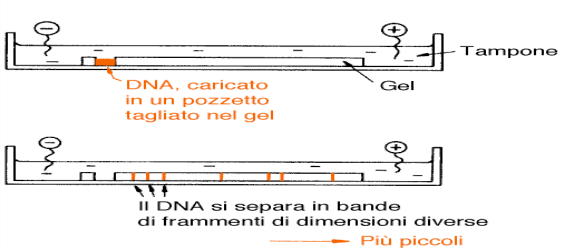
\includegraphics[width=0.6\textwidth]{./immagini/elettroforesi.png}
	\caption{Elettroforesi su GEL}
	\label{elettroforesi}

\end{figure}

\subsubsection{Materiali utilizzati}

\begin{itemize}
	\item Guanti in lattice
	\item Micropipette (100-1000 e 2-200 microlitri)
	\item Beuta da laboratorio
	\item Forno a micronde
	\item Strumenti per l'elettroforesi
	\item Eppendorf
\end{itemize}

\subsubsection{Soluzioni utilizzate}

\begin{itemize}

	\item Miniprep del pUC18
	\item Enzima di restrizione EcoR I
	\item Acqua
	\item Buffer 10X(digestione)
	\item TAE 50X
	\item SyberSafe
	\item Marker (DNA Ladder)

\end{itemize}

\subsection{Procedimento}

\subsubsection{Restrizione del DNA}

\begin{enumerate}

	\item prelevare \SI{10}{\micro\liter} di pUC18 e metterli in una nuova eppendorf
	ed altri \SI{11.5}{\micro\liter} da mettere in un'ulteriore eppendorf per effettuare in
	una provetta la reazione (con l'enzima) e nell'altra il controllo negativo (senza l'enzima).

	\item Addizionare alla eppendorf contenente il nostro plasmide,
	prima \SI{11.5}{\micro\liter} di H\textsubscript{2}O, successivamente
	\SI{2.5}{\micro\liter} di buffer 10X ed infine \SI{1}{\micro\liter} del nostro enzima di restizione EcoR I.

	\item Portare la eppendorf contenente la reazione ad una temperatura di 37°C
	(Temperatura ottimale per l'enzima di restrizione EcoR I) per 1-2 ore,
	in modo che l'enzima EcoR I possa compiere la sua catalizzazione.

\end{enumerate}

\subsubsection{Preparazione ed Elettroforesi}


\begin{enumerate}

	\item Per prima cosa si procede preparando il gel di agarosio 0.8\%, prendendo una beuta
	ed aggiungendo a questa 0.6 g di agarosio, 1.6 ml di TAE 50X e 78.4 ml di H\textsubscript{2}O
	in modo da avere un volume totale di 80 ml.

	\item La miscela a questo punto si presenterà con l'agarosio in fase solida,
	poichè a temperatura ambiente non è solubile.
	Dobbiamo perciò portare la soluzione ad una temperatura prossima all'ebollizione.
	Andremo quindi a scaldare il tutto all'interno di un forno a micronde, prestando attenzione
	che la soluzone non bolla per più di qualche secondo.

	\item Una volta estratta la beuta, facendo attenzione al calore,
	la si mescola fino a che non si otterrà una soluzione omogenea in contenuto e colore.

	\begin{figure}[H]
		\centering
		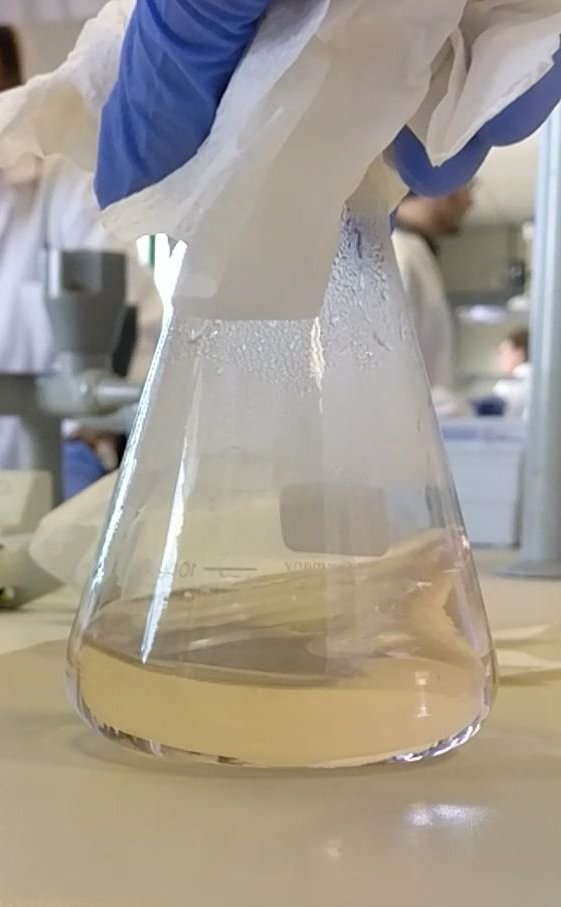
\includegraphics[width=0.3\textwidth]{./immagini/agarosio.jpg}
		\caption{Mescolamento della soluzione con agarosio}
		\label{agarosio}

	\end{figure}

	\item Una volta che la soluzione risulta omogenea e la sua temperatura \`e calata,
	si va ad aggiungere \SI{5}{\micro\liter} di SyberSafe.
	Questo serve come intercalante che si va a legare alla doppia elica
	e sottoposto a raggi UV si rende visibile grazie alla sua fluorescenza.

	\item Andiamo a versare la soluzione nella vaschetta apposita che,
	solidificandosi, ne prende la forma.
	Bisogna inserire il pettine all'interno della vaschetta,
	finch\`e il gel non ha ancora solidificato.
	In questo modo si creeranno i pozzetti dove si andrà a mettere il contenuto delle
	due eppendorf preparate in precedenza una volta che il gel risulter\`a solidificato.

	\begin{figure}[H]

		\centering
		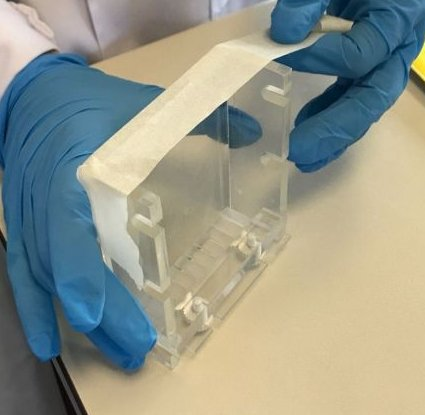
\includegraphics[width=0.3\textwidth]{./immagini/vaschetta.jpg}
		\caption{Vaschetta per solidificazione del gel di agarosio}
		\label{vaschetta}

	\end{figure}


	\item Non appena il gel si sarà solidificato, porlo nella vaschetta togliendo il pettine.
	\item Aggiungere 250 ml di buffer di corsa(TAE 1X) fino al livello indicato.
	\item Caricare all'interno dei pozzetti le varie soluzioni per la corsa elettroforetica tra cui:

	\begin{itemize}

		\item \SI{25}{\micro\liter} di pUC18 digerito (con \SI{5}{\micro\liter} di Loading Buffer)
		\item \SI{25}{\micro\liter} di pUC18 non digerito (con \SI{5}{\micro\liter} di Loading Buffer)
		\item \SI{25}{\micro\liter} di RNA totale derivante dalla scorsa esperienza
		(con \SI{5}{\micro\liter} di Loading Buffer)
		\item Un pozzetto è riservato per il Marker.

	\end{itemize}

	\begin{figure}[H]
		\centering
		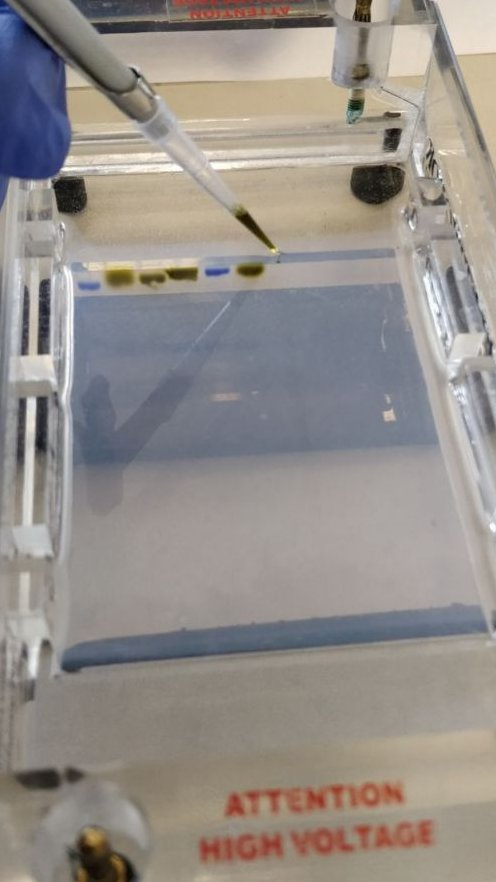
\includegraphics[width=0.3\textwidth]{./immagini/caricamento.jpg}
		\caption{Fase di caricamento dei pozzetti}
		\label{cricamento}
	\end{figure}

	Il Marker è un composto da una miscela di frammenti lineari di DNA con dimensioni
	note che migrano nel gel in prevedibile.
	In questo modo, \`e possibile confrontare il campione con il marker,
	determinando approssimativamente la lunghezza del frammento.

	Il Loading buffer è un colorante con velocità di migrazione nota,
	aggiunto ai composti inseriti nei pozzetti in modo da poter seguire
	l'andamento dell'elettroforesi.

	\begin{figure}[H]

		\centering
		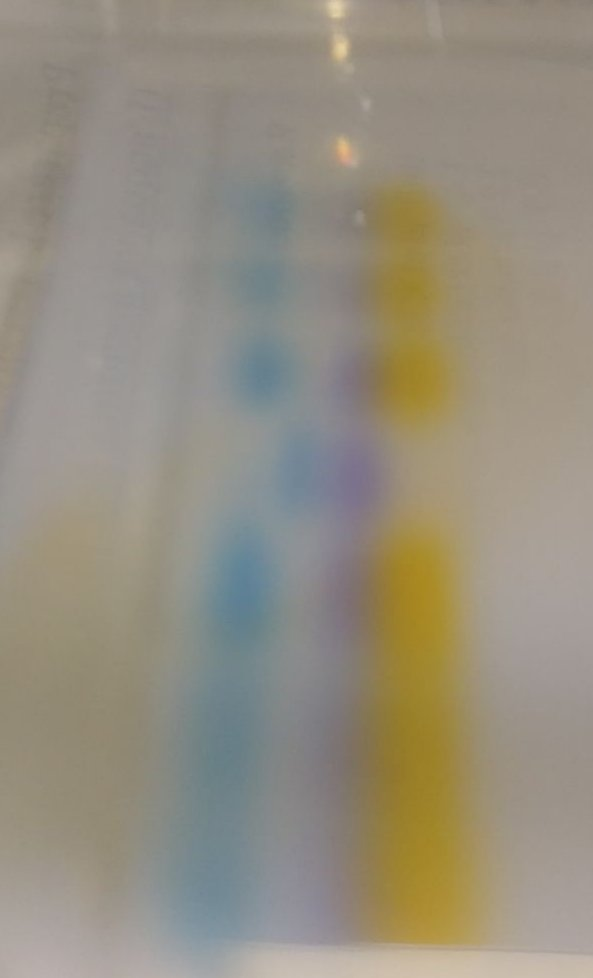
\includegraphics[width=0.3\textwidth]{./immagini/separazione.jpg}
		\caption{Divisione delle bande colorate (Loading buffer)}
		\label{loading_buffer}

	\end{figure}

	\item Caricati i pozzetti chiudere la scatola per l'elettroforesi ed azionare la corrente,
	aspettando il tempo necessario affinch\`e bande risultino ben separate.

	\item Finita la corsa elettroforetica, prendere il gel e metterlo su una piastra
	che emana raggi UV. Coprire con una lastra di vetro che non permetta la fuoriuscita dei raggi UV,
	in modo da non danneggiare gli occhi.
	Avviare la macchina che emette radiazioni UV, in modo da vedere le bande dove il DNA \`e localizzato.
	Confrontandolo con le bande del marker, si pu\`o capire la lunghezza dei vari frammenti.

	\begin{figure}[H]

		\centering
		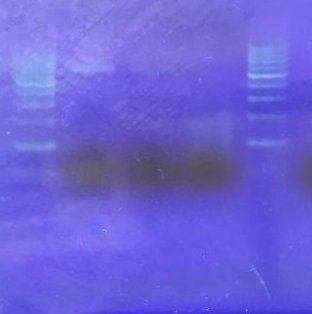
\includegraphics[width=0.3\textwidth]{./immagini/uv.jpg}
		\caption{Fluorescenza del SyberSafe (DNA)}
		\label{SyberSafe}

	\end{figure}



\end{enumerate}


\subsection{Risultati e Conclusioni}

Durante questa esperienza abbiamo capito il funzionamento dell'elettroforesi nei suoi passaggi,
tra cui la preparazione del gel di agarosio, la preparazione e la colorazione delle soluzioni,
il caricamento nei pozzetti di queste e la successiva fluorescenza data dai raggi UV.

Abbiamo compreso poi il processo di digestione tramite gli enzimi di restrizione,
nel nostro caso l'enzima EcoR I.

Andando a guardare l'immagine risultante dalla fluorescenza,
possiamo notare come nei nostri pozzetti,
la quantità di DNA è molto bassa rispetto al
marker (all'interno del primo pozzetto e del sesto pozzetto).
Questo può essere causato da una poca quantità di materiale, oppure qualche errore nella procedura.
Confrontando con le bande del marker possiamo capire all'incirca le dimensioni dei nostri frammenti.

	\newpage

	%_______________________________ESPERIENZA N° 4 (PCR)
	\chapter{Polymerase Chain Reaction (PCR)}

\vspace{0.6cm}


\section{Sommario}

\subsection{Scopo}

In questa esperienza di laboratorio eseguiamo la PCR, una tecnica che fa uso della
DNA polimerasi con lo scopo di amplificare un frammento di DNA ed ottenere così un
ampio numero di copie.\\

\subsection{Cenni teorici}

La PCR è composta da una serie di cicli (con temperature e tempistiche differenti)
che si svolgono in uno specifico macchinario chiamato \textbf{termociclatore},
che permette di eseguire questi cicli in maniera automatica.
Per effettuare la PCR inoltre prepareremo un gel di agarosio 0,8\%
su cui avverrà la corsa elettroforetica.

\subsection{Materiali utilizzati}

\begin{itemize}
	\item Eppendorf
	\item Micropipette
	\item Forno microonde
	\item Vaschetta per Elettroforesi
	\item Lampada UV
	\item Beuta
\end{itemize}

\subsection{Soluzioni utilizzate}
\begin{itemize}
	\item H$_2$O sterile
	\item Buffer TAQ 10X
	\item MgCl$_2$
	\item Primer FOR
	\item Primer REV
	\item DNA plasmidico contenente l'inserto da amplificare (GPR3), circa 1000bp
	\item TAQ polimerasi
\end{itemize}

\section{Procedimento}

\subsection{Preparazione PCR}

Prendiamo una eppendorf da 250 $\mu$l in cui bisogna aggiungere (Attenzione a non contaminare):
\begin{itemize}
	\item 12 $\mu$l H2O sterile
	\item 2 $\mu$l buffer TAQ (10X)
	\item 1 $\mu$l MgCl2 (50mM)
	\item 1 $\mu$l Primer FOR (25 $\mu$M)
	\item 1 $\mu$l Primer REV (25 $\mu$M)
	\item 1 $\mu$l dNTPs (10 mM)
	\item 1 $\mu$l DNA plasmidico contenente l’inserto da amplificare (GPR3), circa 1000 bp
	\item 1 $\mu$l TAQ polimerasi
\end{itemize}

Totale 20 $\mu$l\\

Il mix ottenuto nella eppendorf
viene inserito nel termociclatore, i cui cocli sono specificati nella figura \ref{cicli_termociclatore}.
\begin{figure}[htbp]
	\centering
	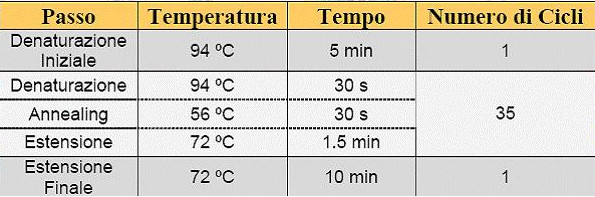
\includegraphics[width=80mm]{./immagini/cicli_termociclatore.jpg}
	\caption{Cicli termociclatore}
	\label{cicli_termociclatore}
\end{figure}

\subsection{Preparazione gel di agarosio 0,8\%}

Passiamo alla preparazione del gel di Agarosio 0,8\% per la corsa elettroforetica.
Pesiamo le seguenti quantità per un gel allo 0,8\% in una beuta:

\begin{itemize}
	\item 0,6 g  di agarosio
	\item 1,6  ml TAE 50X
	\item 78,4 ml H2O
\end{itemize}

Totale 80 ml
\begin{enumerate}
\item Scaldare nel forno a microonde la beuta con i componenti facendo attenzione a
non portare ad ebollizione, mescolando ogni tanto per sciogliere bene.
\item Aggiungere 5 $\mu$l di SyberSafe.
\item Mescolare e versare nell’apposita vaschetta
usando il pettine per creare i pozzetti.
\item A gel solidificato togliere il pettine e
aggiungere 250 ml di buffer di corsa (TAE 1X).

\item Preparato il gel nella camera per l’elettroforesi caricare nei pozzetti la
soluzione preparata in precedenza dopo che il termociclatore ha terminato il
lavoro.
\item Avviare la corsa elettroforetica.

\item Finita la corsa elettroforetica, con l’ausilio di una lampada UV, osservare il
risultato ottenuto.

\end{enumerate}


\section{Risultati e Conclusioni}

Controllando la fluorescenza possiamo capire l'efficacia della replicazione
ottenuta. Confrontando il pozzetto caricato da noi con un secondo pozzetto
dove è presente un marker possiamo capire se la PCR ha replicato il nostro
frammento di DNA o anche altri frammenti aspecifici.

\begin{figure}[htbp]
	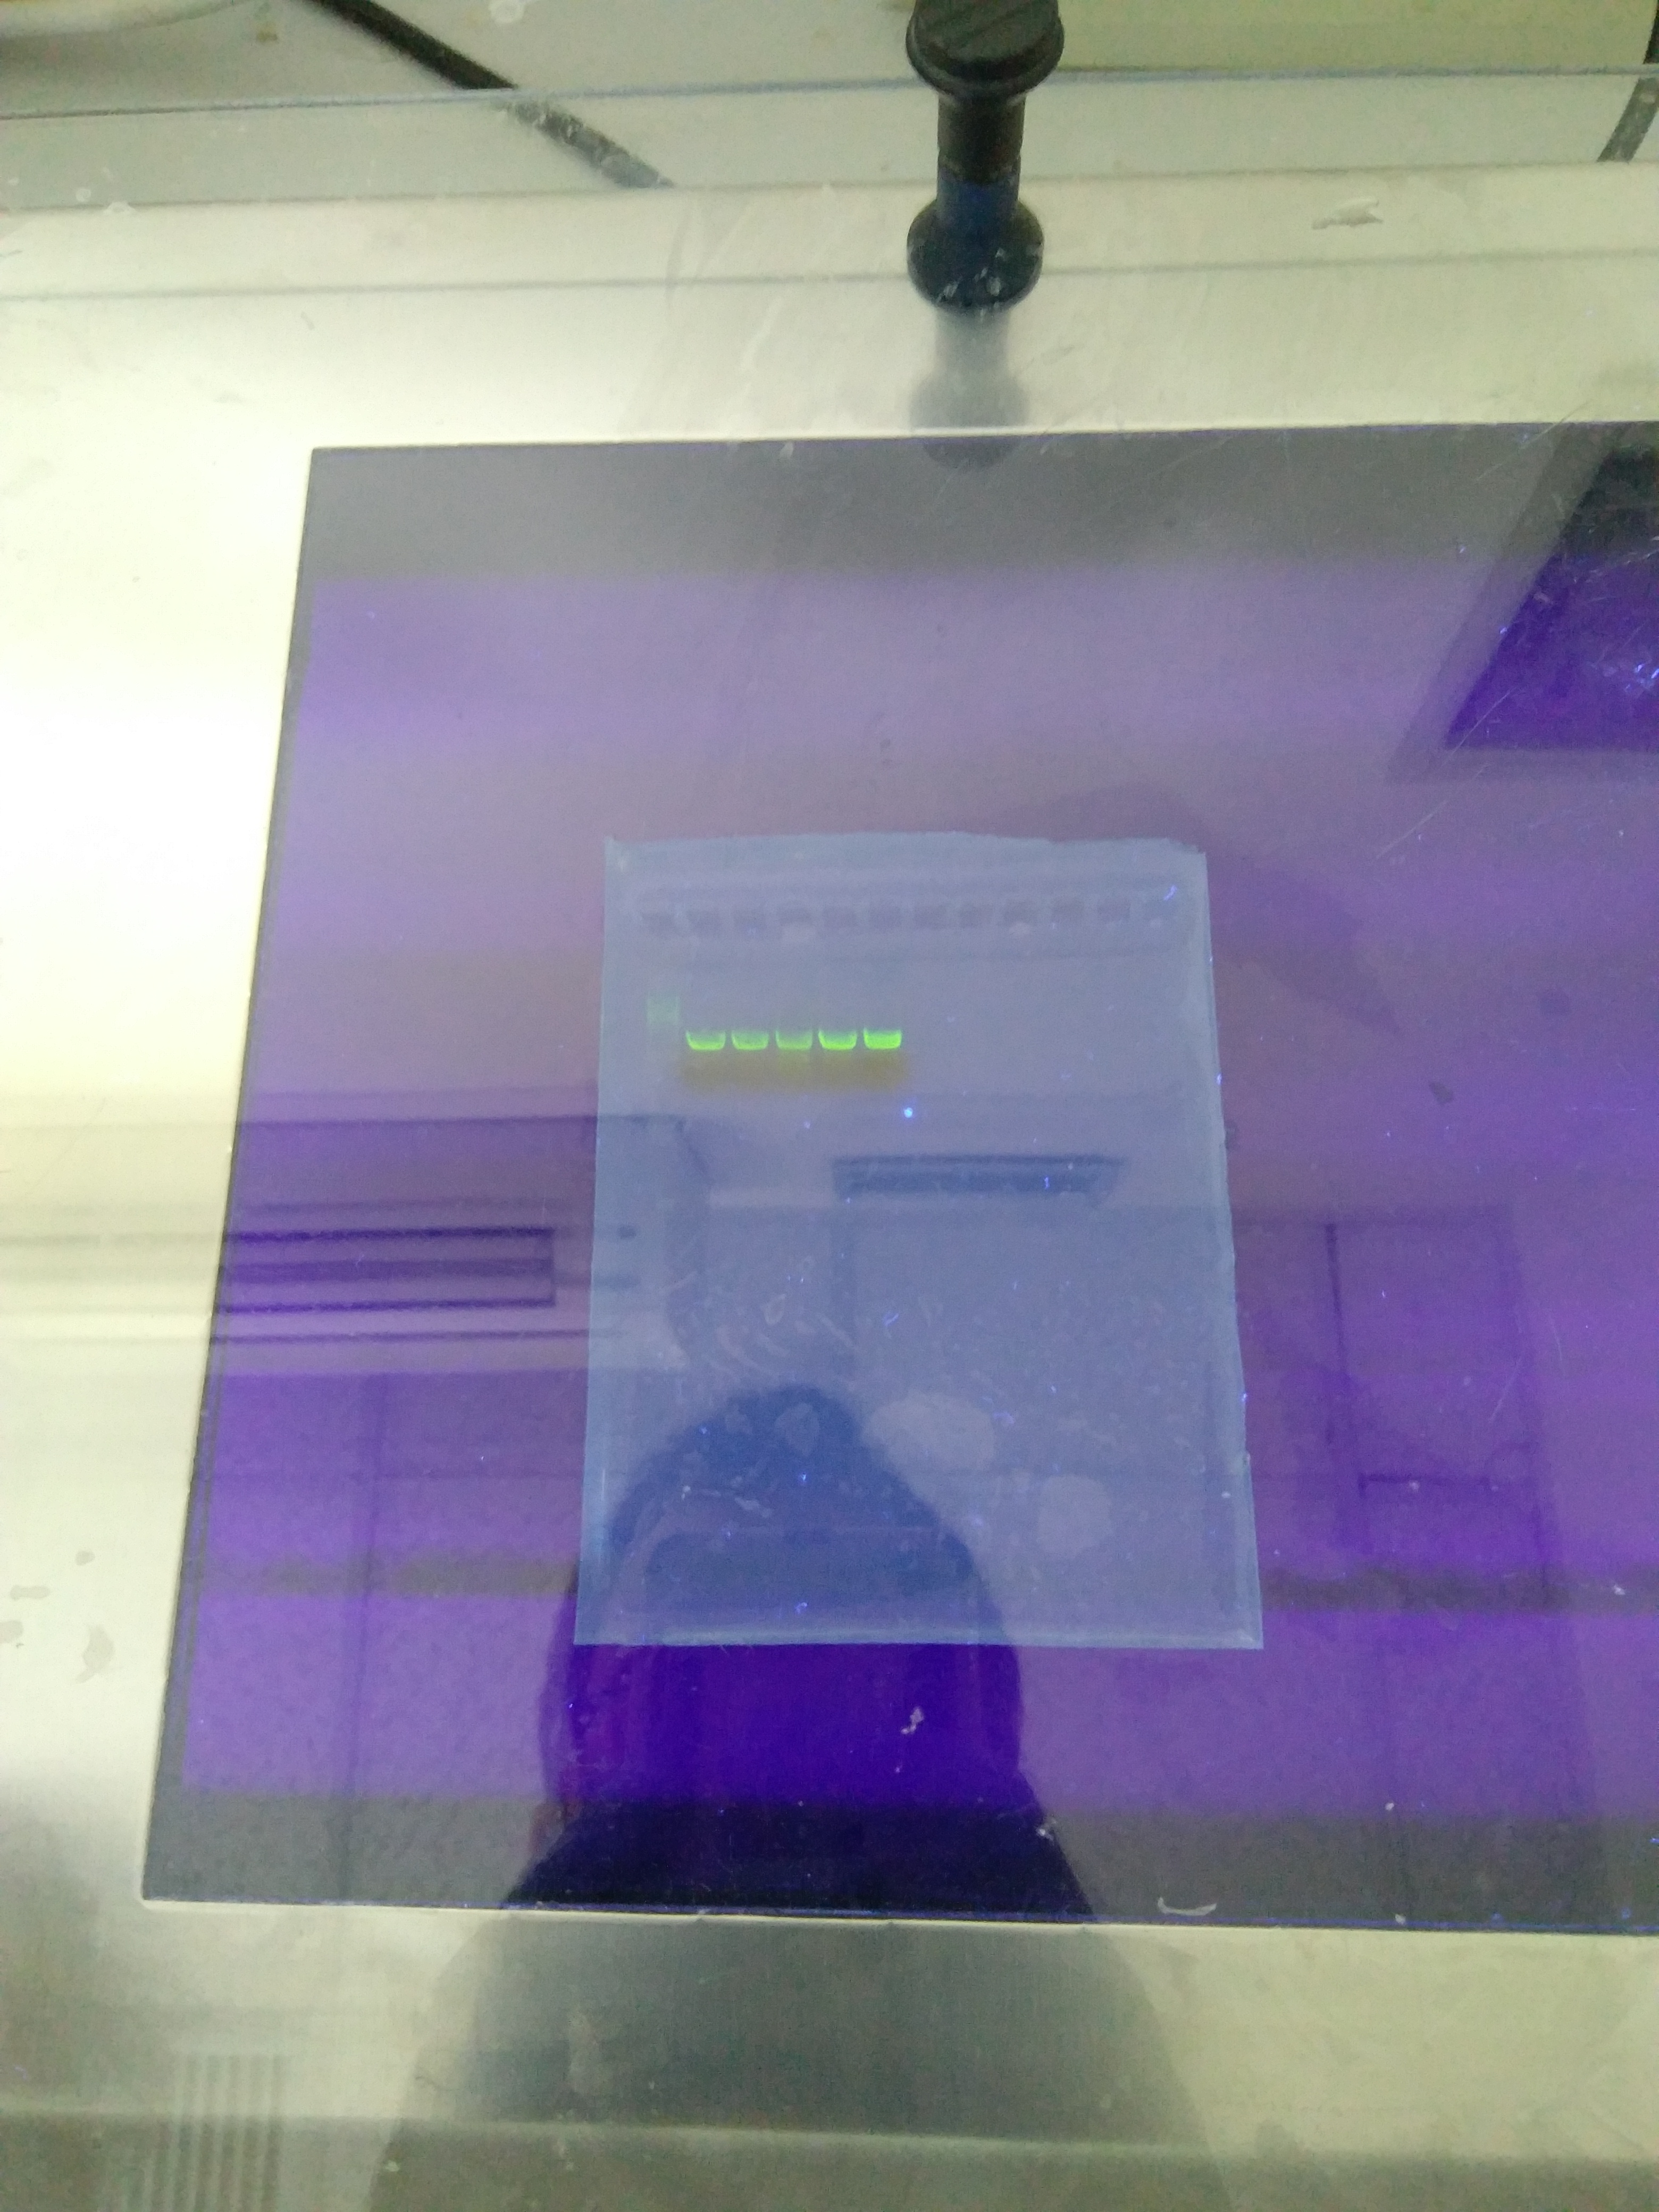
\includegraphics[width=50mm]{./immagini/risultato_pcr.jpg}
	\caption{Risultato della PCR}
	\label{risultato_pcr}
\end{figure}

	\newpage

	%_______________________________ESPERIENZA N° 5 (PREPARAZONE TERRENO (E PIASTRAGGIO) E CELLULE COMPETENTI)
	\section{\LARGE{Preparazione di:  terreno LB solido, cellule competenti e piastre LB-agar }}

\vspace{0.6cm}


\subsection{Sommario}

\subsubsection{Scopo}

Quest'esperienza in laboratorio si divide in tre fasi: Una prima fase che consiste nella preparazione del terreno di cultura dove andranno a crescere le nostre cellule batteriche; Una seconda fase consistente nella preparazione delle cellule competenti; E infine l'ultima fase consiste nella preparazione delle piastre di LB-agar, dove andremo a mettere il terreno e infine dove cresceranno i nostri batteri.


\subsubsection{Cenni teorici}

\textbf{Colture batteriche}
\vspace{0.3cm}

All'interno dei laboratori, i ceppi che comunemente si usano sono dei ceppi che derivano dal batterio di E.coli, che è un batterio gram negativo non patogeno, che viene selezionato e modificato.
A seconda del genotipo, cioè con mutazioni su particolari geni o introduzione di geni estranei, vengono utilizzati per diversi scopi, però in generale si possono dividere in questo modo:
\begin{itemize}
  \item Ceppi di propagazione, atti al clonaggio o alla propagazione di plasmidi;

  \item Ceppi di espressione, atti ad esprimere le proteine ricombinanti.

\end{itemize}

\begin{figure}[H]

  \centering
  \subfloat{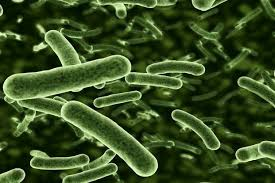
\includegraphics[width=0.3\textwidth]{./immagini/e_coli.jpeg}} \quad
  \subfloat{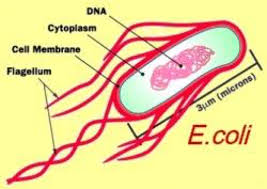
\includegraphics[width=0.3\textwidth]{./immagini/e_coli1.jpeg}}
  \caption{vista al microscopio del batterio di Eschericchia coli (destra) e suddivisione di questo batterio (sinistra)}
  \label{e_coli}

\end{figure}

\textbf{Terreni di cultura}
\vspace{0.3cm}

I terreni di cultura, sono le soluzioni solide o liquide contenenti sostanze nutritive su cui è possibile crescere delle cellule eucariotiche (come E.coli) e procariotiche.
Una possibile suddivisione può essere:

\begin{tabular}{ll}
\hline
\multicolumn{1}{c}{Stato fisico}

& -\textbf{LIQUIDI}: componenti sciolti in acqua e sterilizzati; \\ \cline{1-1} &usati per crescita delle cellule;\\&  espressione di proteine ricombinanti ecc..\\

& -\textbf{SOLIDI}:  possono essere naturalmente tali (terreno alla patata)\\ & o vengono solidificati per aggiunta di un agente gelificante (agar, gelatina). \\ &selezioni di cloni mediate isolamento di
singole colonie, propagazione \\ & delle colonie o della linea cellulare \\

\hline
\multicolumn{1}{c}{Costituzione chimica}

& -\textbf{MINIMI}: Per la crescita dei soli batteri autotrofi. Gli elementi \\ \cline{1-1} & essenziali (N, C, S, P) sono presenti come sali inorganici\\ & in composizione e quantità note.\\
& -\textbf{SINTETICI}(Definiti) : nota la formulazione chimica di ogni ingrediente; \\ & le singole sostanze di cui il batterio necessita sono presenti in quantità note.\\
& -\textbf{COMPLESSI}: Ignota l’esatta composizione chimica delle sostanze nutritive \\ & (estratto di carne di bue, cuore, cervello, ecc.), benché chimicamente non definite.\\ & Comprendono la maggior parte dei terreni usati in laboratorio. \\ & in  questa sezone c'è il terreno LB(Luria Bertani medium).\\ &  Questi terreni sono utilizzati per la crescita di cellule e per l’espressione
\\ & di proteine ricombinanti non modificate.\\

\hline
\multicolumn{1}{c}{Funzione}

& -\textbf{ARRICCHIMENTO}(ELETTIVI): la specie microbica di interesse vi cresce in \\ \cline{1-1} & un tempo assai più breve rispetto ad altre specie microbiche.\\
& -\textbf{SELETTIVI}: Contengono sostanze batteriostatiche (sali biliari, NaCl) \\ &  a concentrazione nota che inibiscono o rallentano lo sviluppo \\ & di molte specie microbiche. \\ &  Utilizzati per isolare specifici microrganismi da campioni altamente contaminati.\\
& -\textbf{DIFFERENZIALI}: Contengono sostanze indicatrici di particolari reazioni \\ & biochimiche che avvengono nel terreno stesso. \\ & Usati per la identificazione di specifici microrganismi.\\


\end{tabular}

\textbf{Piastra agar}
\vspace{0.3cm}

Una \textbf{piastra Agar} è un disco di Petri sterile che contiene nutrimenti di crescita (tipicamente agar + nutrienti) usati per coltivare micro-organismi o piccole piante.
componenti di crescita selettivi, si possono aggiungere agli altri come per esempo antibiotici.




\subsubsection{Materiali utilizzati}

\begin{itemize}
	\item Guanti in lattice
	\item Micropipette (100-1000 e 2-200 microlitri)
	\item Bottiglia da laboratorio
  \item Piastre di Petri
	\item Forno a micronde
  \item provetta Falcon da 50mL
  \item provetta eppendorf 2mL

\end{itemize}

\subsubsection{Soluzioni utilizzate}

\begin{itemize}

  \item Soluzione Buffer I:
  \begin{enumerate}
    \item RbCl 12 g/l (0.6g)
    \item MnCl*4H\textsubscript{2}O 9.9 g/l (0.49g)
    \item 1.5 ml di una soluzione di KAc 1M a pH 7.5
    \item CaCl\textsubscript{2}*2H\textsubscript{2}O 1.5 g/l (0.075g)
    \item Glicerolo 150 g/l (7.5g)
    \item Si porta a pH 5.8 con HAc, si porta a volume (50ml) con acqua milliQ e si filtra con una membrana a pori di 0.22 \SI{250}{\micro\liter} sotto cappa.
  \end{enumerate}
  \item Soluzione Buffer II:
  \begin{enumerate}
    \item 0.4 ml di una soluzione di MOPS 0.5 M a pH 6.8
    \item RbCl 1.2 g/l (0.025g)
    \item CaCl\textsubscript{2}*2H\textsubscript{2}O 11 g/l (0.22g)
    \item Glicerolo 150 g/l (3g)
    \item Si porta a volume (20ml) con acqua milliQ e si filtra con una membrana con pori di 0.22 \SI{250}{\micro\liter} sotto cappa.
  \end{enumerate}

\end{itemize}

\subsection{Procedimento}

\subsubsection{Preparazione del terreno LS-solido}

La composizione del terreno LB(Luria-Bertani) medium è di :

\begin{itemize}
  \item 1\% Tryptone
  \item 0.5\% Estratto di lievito
  \item 0.5\% inattaccabile
  \item 1.5\% Agar batteriologico
\end{itemize}

Per la preparazione di questo terreno bisogna eseguire questi passaggi:

\begin{enumerate}

	\item Pesare le quantità necessarie cioè prendere: 0.5g di tryptone, 0.25g di estratto di lievito, 0.025g di NaCl e 0.75g di agar batteriologico e metterle in una beuta portando a volume 50mL con acqua distillata.
  \item Attaccare alla mia bottiglia da laboratorio un autoclave, cioè un pezzo di scotch ma che si va a marcare quando la sua temperatura raggiunge i 100°C, questo serve per sapere se la nostra bottiglia, una volta inserita nella chiusura autoclave raggiunge la temperatura adatta per la nostra reazione.

	\item Poratare la Bottiglia all'interno dell' autoclave, cioè una macchina che è molto simile al funzionamento di una pentola a pressione, nella quale il contenuto delle bottigliepotrà raggiungere la giusta temperatura per la reazione.

  \begin{figure}[H]
		\centering
		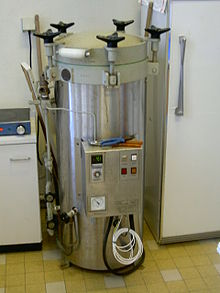
\includegraphics[width=0.3\textwidth]{./immagini/autoclave.JPG}
		\caption{Autoclave}
		\label{autoclave}

	\end{figure}


\end{enumerate}



\subsubsection{Preparazione delle cellule competenti}


\begin{enumerate}

	\item Prelevare sotto cappa biologica 5 mL di una coltura di cellule i E. coli DH5a ed OD 600 di 0.3-0.4 e trasferirli in una provetta Falcon da 50 mL sterile;

  \item Portare la provetta Falcon con le cellule di E.coli all'interno della centrifuga, e centrifugare per 5 minuti a 3000 g, a 4°C;

  \item Prelevare la falcon centrifugata ed eliminare il surnatante, semplicemente rovesciando il contenuto. Le nostre cellule staranno ancorate in fondo alla provetta Falcon raggruppate, formando un pellet;

  \item Risospendere le cellule in 0.8mL di buffer I;

  \item Trasferire il contenuto in una provetta eppendorf da 2mL sotto cappa biologica;

  \item Incubare in ghiaccio per 15 minuti;

  \item Passati i 15 minuti si riprende la provetta eppendorf e la si fa centrifugare per 5 minuti a 3000g a 4°C;

  \item Andare sotto cappa bilogica per eliminare il surnatante e risospendere le cellule in \SI{400}{\micro\liter} di buffer II

  \item Congelare in N\textsubscript2 liquido e conservare a -80°C, questo passaggio viene effettuato con N\textsubscript2 liquido perchè il passaggio di temperatura deve avvenire molto velocemente per garantire che le nostre cellule diventino competenti;

\end{enumerate}

\subsubsection{Preparazione delle piastre di LB-agar}

Una volta che le bottiglie all'interno dell'autoclave sono state tolte, si prendono senza farle raffreddare troppo perchè senò la miscla si solidifica ed andando sotto cappa biologica
aggiungiamo 100 \SI{100}{\micro\gram}/ml di ampicillina (\SI{50}{\micro\liter} dello stock 1000X). Una volta mescolato abbastanza, Si versa il terreno dalle bottiglie alle due pistre di Petri, Lasciandole
aperte sotto cappa fino a che l'agar non solidifica. Una volta che l'agar si è solidificato si conservano a 4°C.


\subsection{Risultati e Conclusioni}

Durante questa esperienza, abbiamo capito come preparare un terreno di coltura batterico, specialemtne un terreno solido LB, contenente ampicillina, che nella prossima esperienza capiremo a cosa serve;
Abbiamo preparato poi delle cellule competenti, in grado di poter integrare del materiale genetico proveniente da un ambiente extracellulare;
Ed infine abbiamo perparato una piastra di Petri con il nostro terreno mixato in precedenza.

	\newpage

	%_______________________________ESPERIENZA N° 6 (XL1_BLUE)
	\section{\LARGE{Trasformazione delle cellule di escherichia coli xl1 blue}}

\vspace{0.6cm}

\subsection{Sommario}

\subsubsection{Scopo}

L'obiettivo di questa esperienza è quello di manipolare le \textbf{culture batteriche di E.coli}
(batterio gram negativo non patogeno usato comunemente nei laboratori di ricerca),
andando a \textbf{trasportare il plasmide pUC18}, precedentemente trattato,
all'interno di questi batteri diventando cos\`i un ceppo di propagazione
(atto al clonaggio e alla propagazione di plasmidi) all'interno di un terreno di crescita.

\subsubsection{Cenni teorici}

Il procedimento di trasporto del dsDNA da esterno alla cellula all'interno è chiamato
\textbf{trasformazione batterica}, ed è un fenomeno parasessuale che consente ai batteri
lo scambio di materiale genico.

Solo alcune specie batteriche possono acquisire DNA estraneo dall'ambiente (DNA esogeno)
che deve essere a doppia elica, con facilità.
Queste sono dette cellule \textit{"naturalmente competenti"}.
Altre specie invece diventano competenti solo in particolari condizioni fisiologiche
ed altre ancora, come per esempio E.coli, necessitano di una trasformazione artificiale in
laboratorio tramite vari metodi chimici o fisici
(da noi usato è il metodo dello \textit{shock-termico}) che le rende \textbf{competenti}.

Una volta che il plasmide si trova all'interno della cellula batterica di E.coli,
la si fa crescere all'interno di piastre precedentemente preparate con LB-agar-amp
(Luria Bertani medium with ampicillin), in grado di fornire il nutrimento necessario
alla cellula per potersi nutrire e clonare,
producendo molte copie contenenti molti plasmidi ingegnerizzati di nostro interesse.

\subsection{Materiali utilizzati}

\begin{itemize}
	\item Guanti in lattice
	\item Provette Eppendorf (2mL)
	\item Micropipette (100-1000  e 2-200 microlitri  )
	\item Scatola di polistirolo contenente ghiaccio
	\item Bagno termostatico
	\item Piasra di LB-agar-amp
	\item Bacchette in vetro
\end{itemize}

\subsection{Soluzioni utilizate}

\begin{itemize}
	\item Miniprep del pUC18
	\item Cellule competenti
	\item LB liquido
\end{itemize}

\subsection{Procedimento}

\begin{enumerate}
	\item Diluire la nostra miniprep del pUC18 (descritta nell'esperienza numero 1)
  in acqua pura in misura 1:10 quindi prelevare 1$\mu$l di miniprep del pUC18 e
  9$\mu$l di acqua pura tramite una micropipetta e inserire le due componenti
  in una nuova provetta eppendorf da 2 ml. \\
  Questa diluizione \`e necessaria per avere un totale di 10$\mu$l.


	\item Prelevare in un \textit{ambiente biologicamente sterile} (sotto cappa biologica) 100 microlitri
  di cellule competenti e metterli in una provetta eppendorf da 2 ml.
  Lavorando in un ambiente sterile si garantisce la protezione da agenti inquinanti derivanti dall’esterno.

	\item Aggiungere 1$\mu$l della miniprep, diluita con acqua al passo n° 1,
  all'interno della eppendorf contenente le cellule competenti.
  In questo modo si forma una soluzione sia di cellule batteriche che di plasmidi,
  che dovranno poi entrare all'interno delle cellule.

	\item Agitare la soluzione per far s\`i che i plasmidi si distribuiscano in
  modo uniforme.
  \item Incubare la provetta contenente la soluzione in ghiaccio per una trentina di minuti
  in modo che la temperatura si abbassi gradualmente di qualche grado e che i plasmidi
  si vadano a legare sulla membrana della cellula batterica.

	\item Attendere 30' in modo che la temperatura della soluzione contenente cellule e plasmidi si è abbassi
  e stabilizzi.
  \item Ora linea teorica i plasmidi sono ancorati alle membrane delle cellule dove dovranno poi essere
  incorporati.
  \item A questo punto effettuare lo \textbf{shock termico}, portando la provetta eppendorf
  da una temperatura di ca. 0°C(ghiaccio) ad una temperatura di 42°C  molto rapidamente e lasciarla
  nel bagno termostatico per 1 minuto (la tempistica è importante poichè se si lascia il tutto ad una
  temperatura elevata per troppo tempo le cellule batteriche potrebbero morire).
  Questa operazione \`e di cruciale importanza, infatti fa in modo che sulle membrane delle cellule batteriche
  di E.coli si \textit{aprano dei pori}, permettendo il passaggio del DNA esogeno (plasmide) all'interno
  formando così una \textbf{cellula trasformata}.
	Un altro metodo per effettuare l'apertura dei pori e la successiva immissione dei plasmidi all'interno
  delle cellule competenti è l'elettroporazione che consiste in una repentina scarica elettrica
  ad alto voltaggio. Il vantaggio di questa tecnica \`e che può essere applicata anche a cellule eucariotiche.

	\begin{figure}[H]
		\centering
		\subfloat{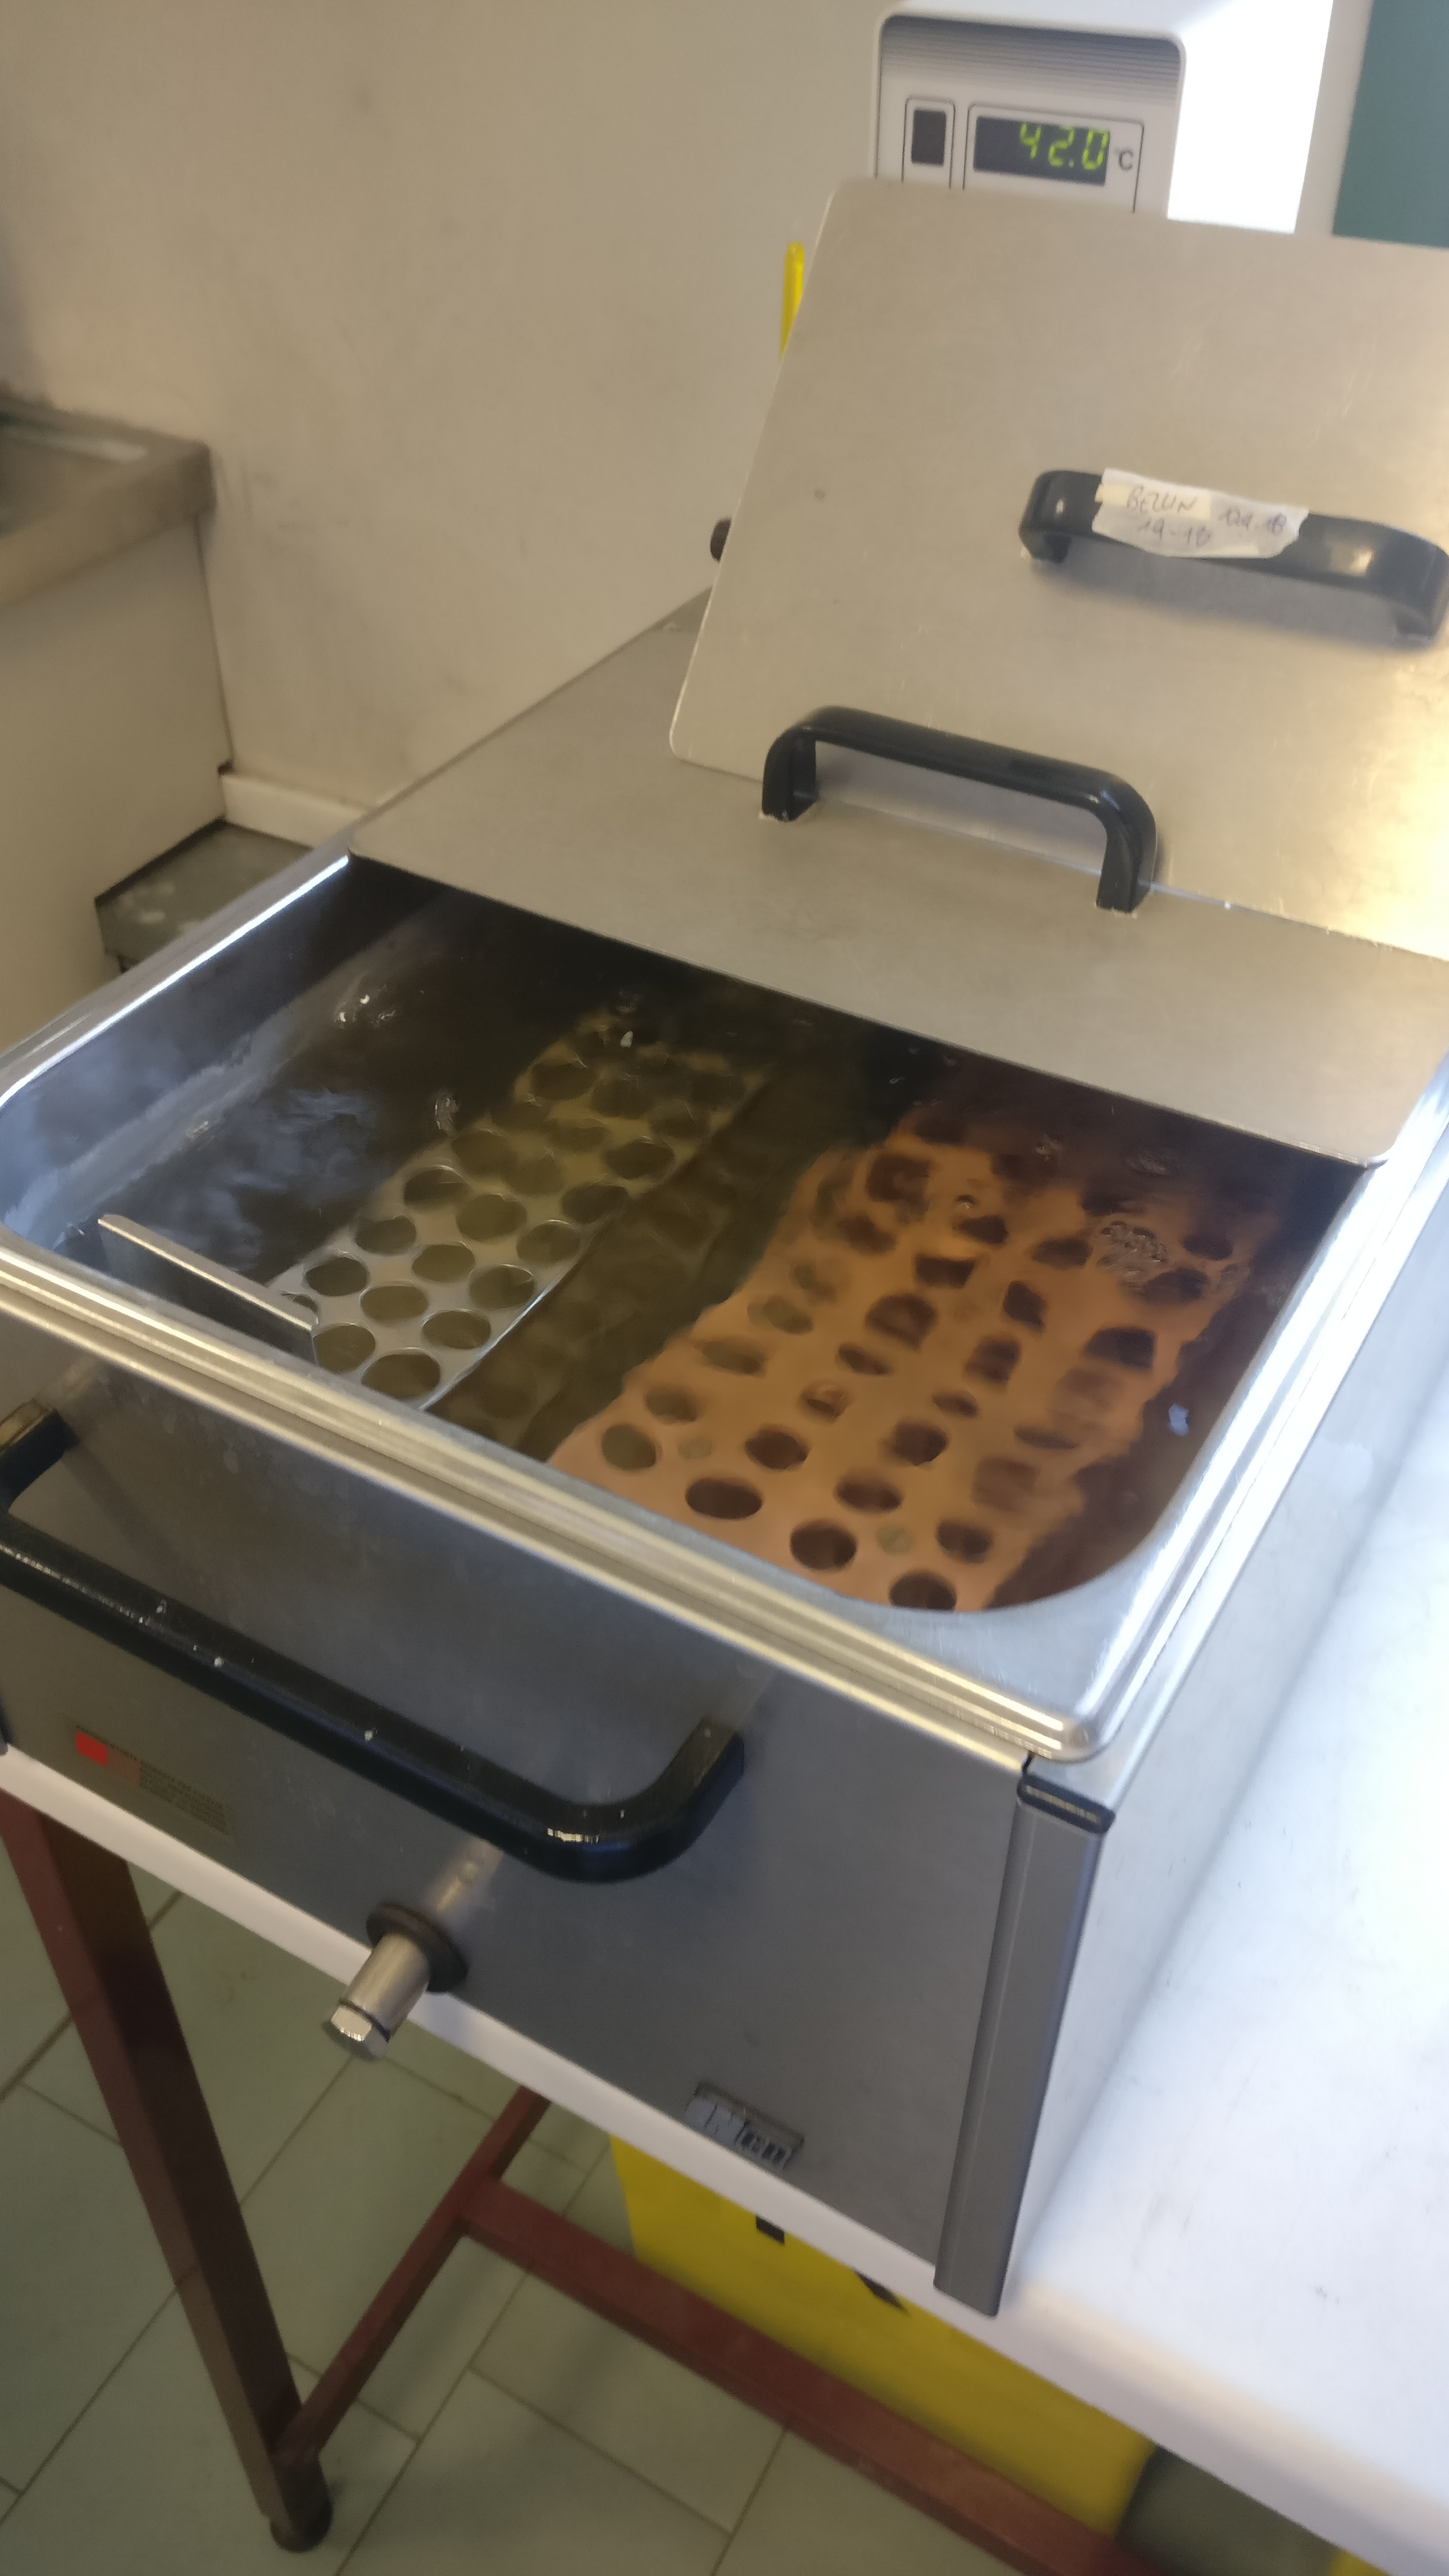
\includegraphics[width=0.3\textwidth]{./immagini/bagno_termostatico.jpg}} \quad
		\subfloat{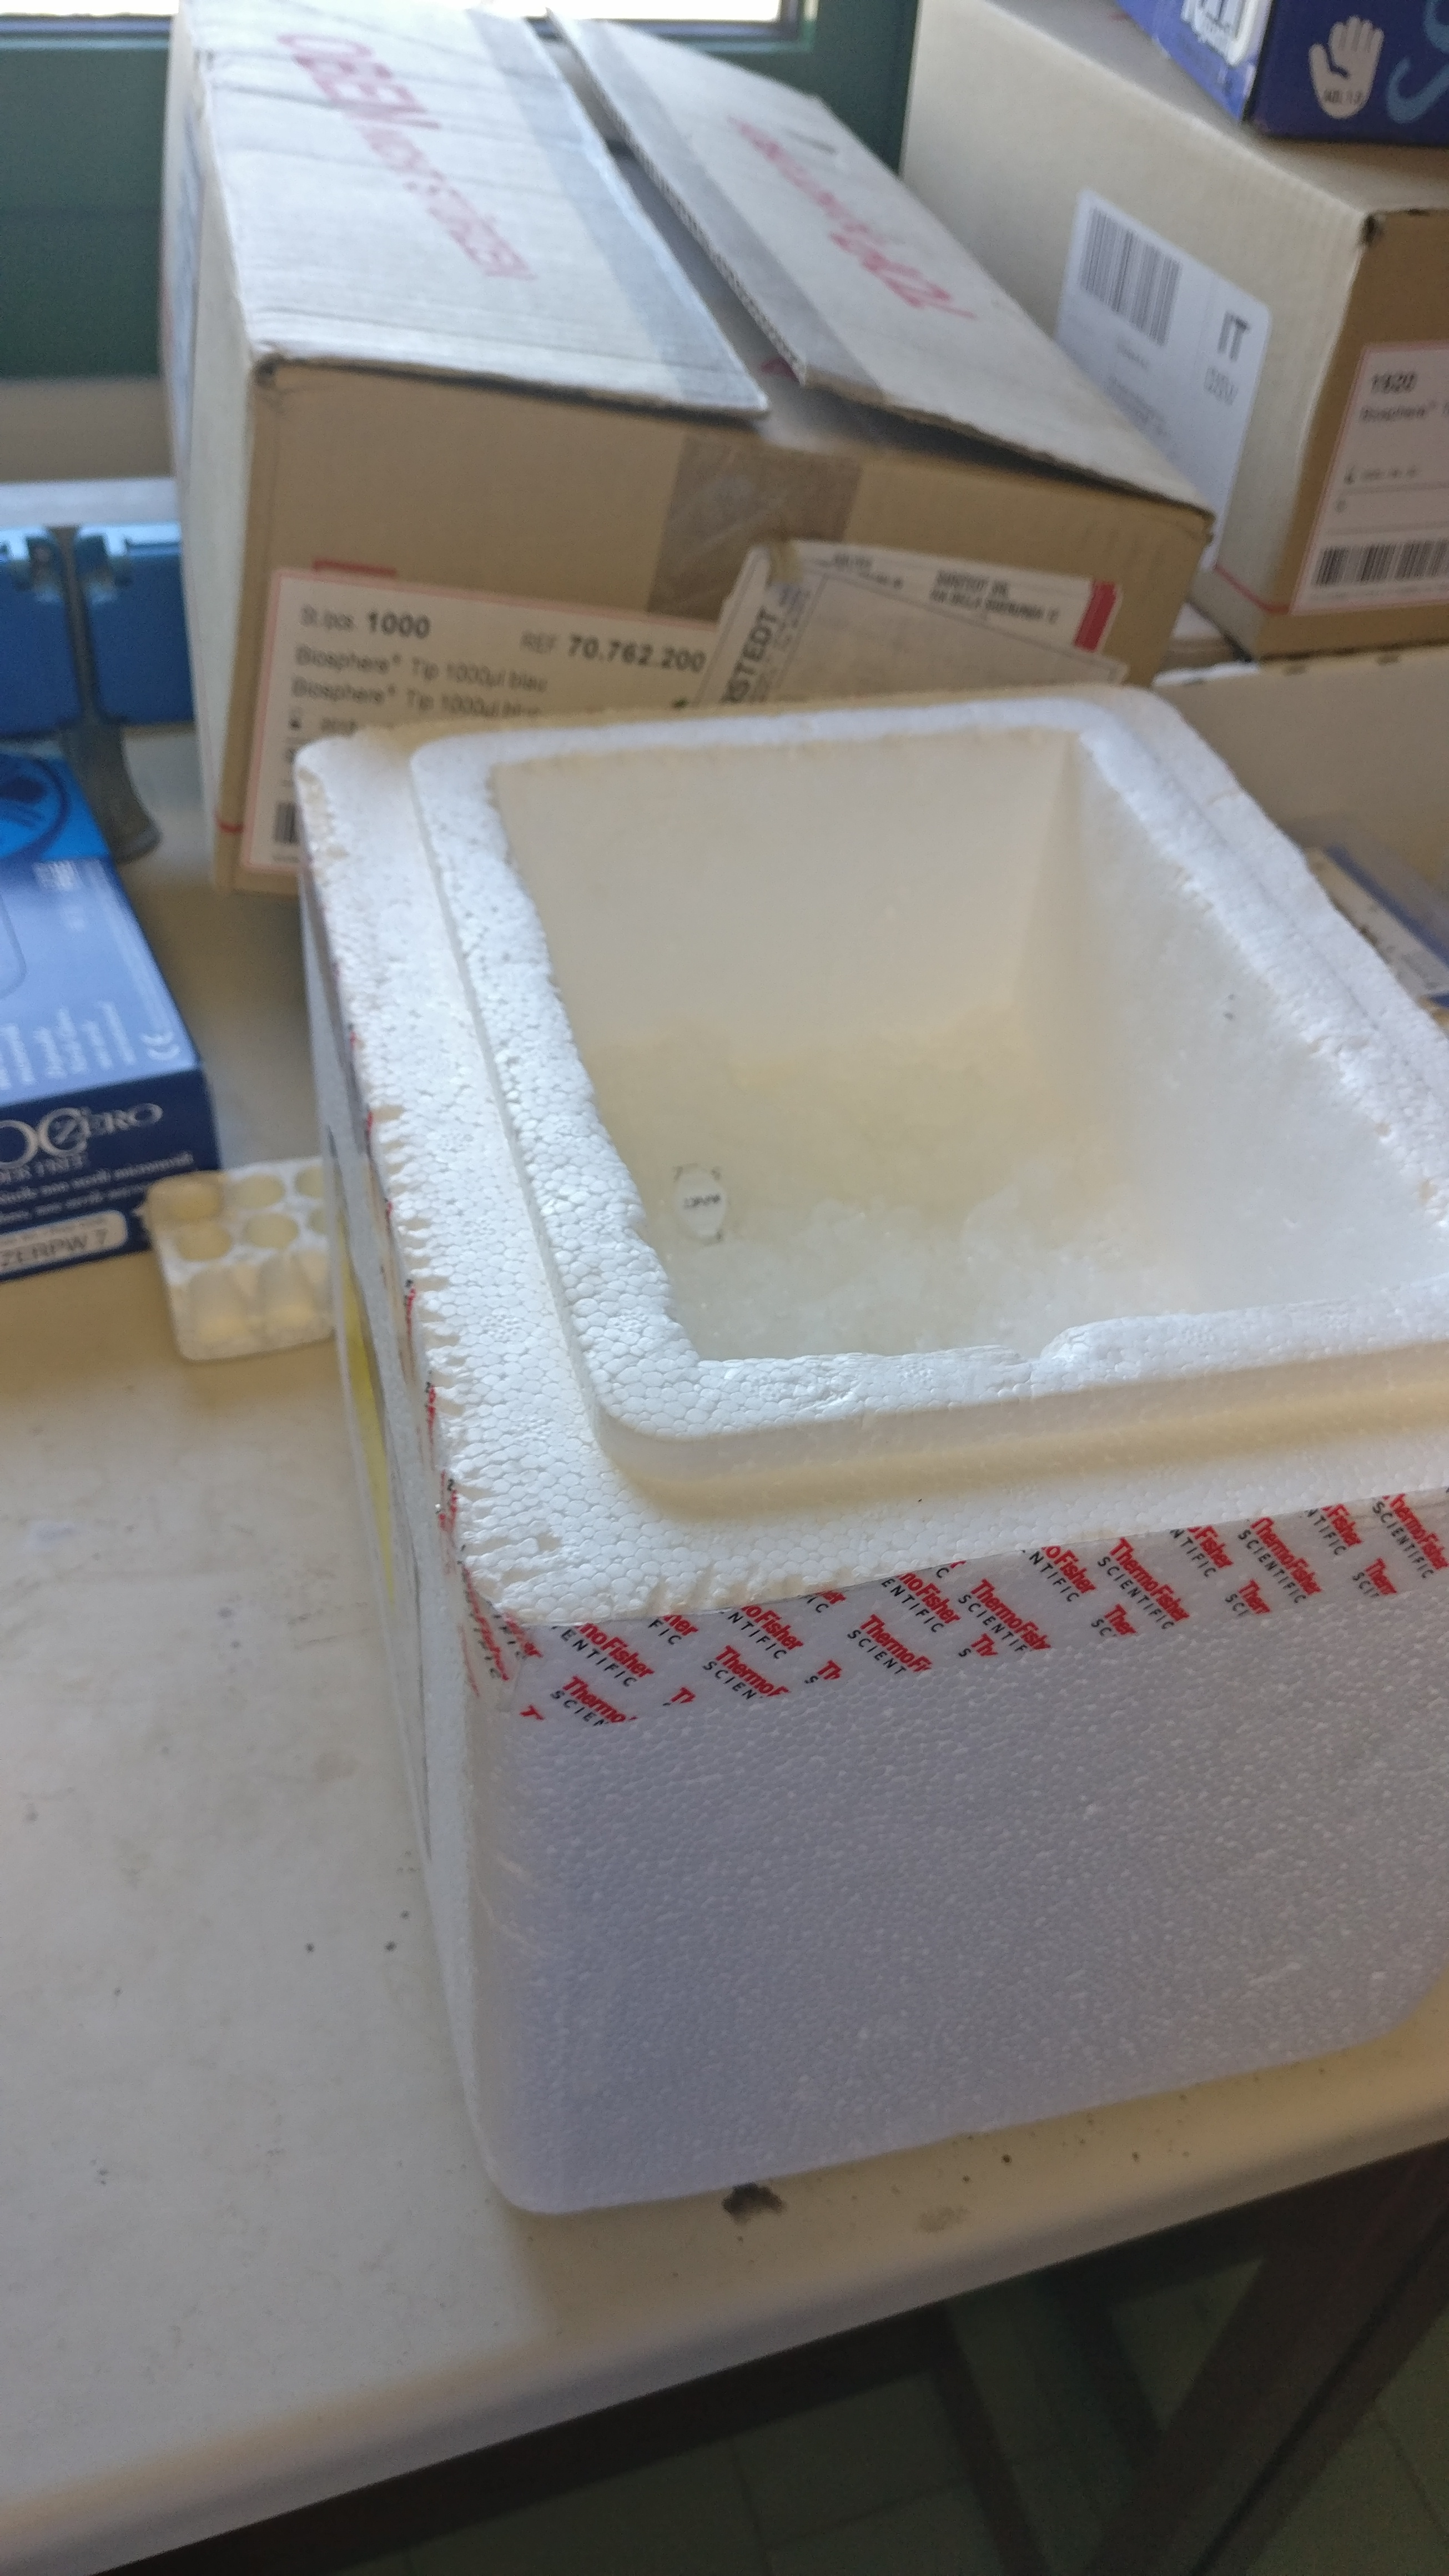
\includegraphics[width=0.3\textwidth]{./immagini/ghiaccio.jpg}}
		\caption{Bagno termostatico e immersione in ghiaccio}
		\label{bagno_e_ghiaccio}
	\end{figure}
	\item Passato un minuto prendere la eppendorf e rimetterla in ghiaccio per altri 5 minuti,
  favorendo il \textit{rallentamento del metabolismo cellulare}.
	\item Aggiungere del nutriente LB liquido all'interno della provetta, e incubarla a 37°C per 1 ora.
   In questo modo la cultura batterica si accresce e si esprime la \textbf{resistenza all'antibiotico}
   (ampicillina, codificata dal gene contenuto all'interno del plasmide).
    Una volta messo sul terreno di LB-amp, questo ci permette di sapere se il nostro plasmide è
    stato effettivamente incorporato all'interno della cellula batterica o no.
	\vspace{0.3cm}

	\begin{figure}[H]

		\centering
		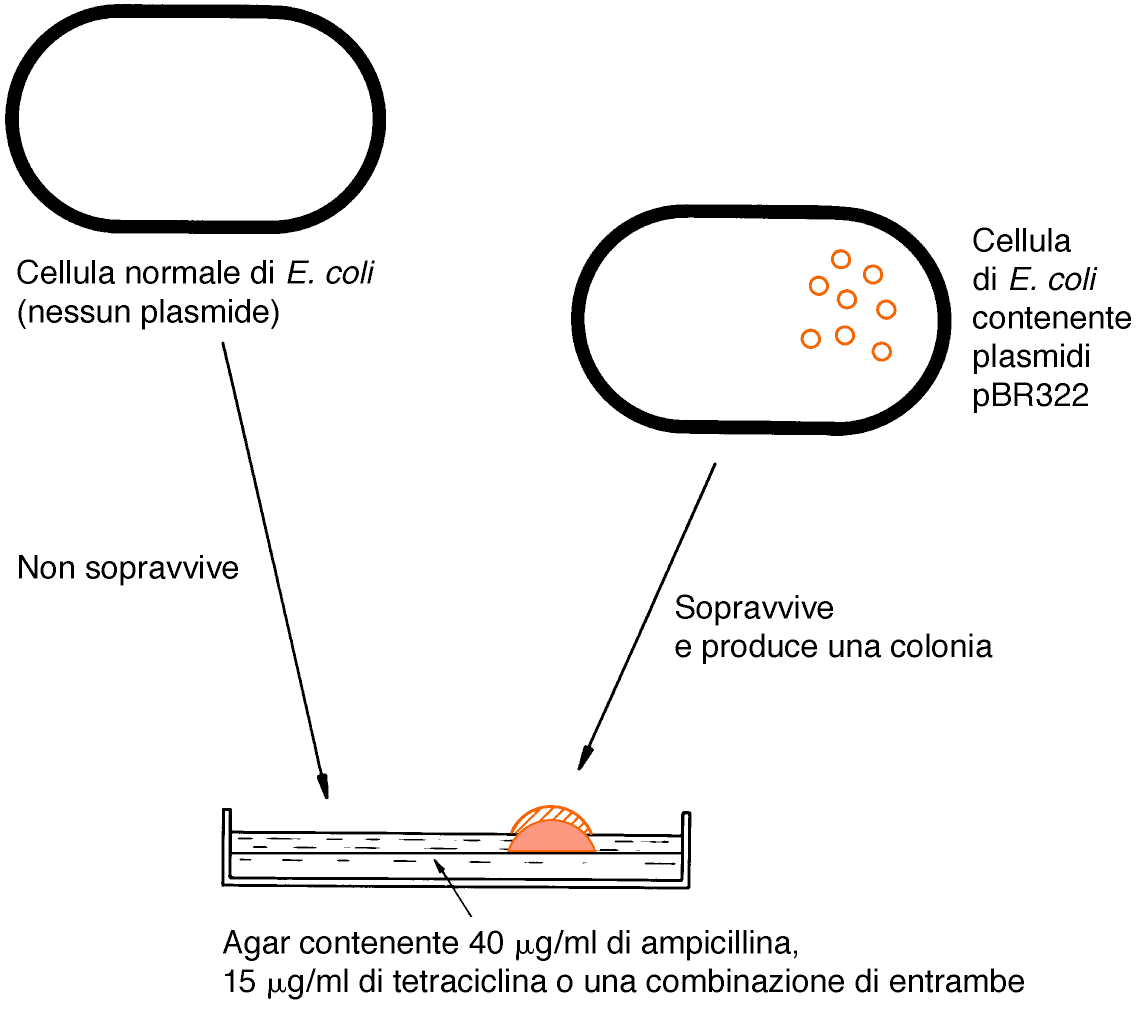
\includegraphics[width=0.6\textwidth]{./immagini/resistenza_ampicillina.png}
		\caption{Colonie con il plasmide integrato resistono al terreno con ampicillina }
		\label{resistenza ampicillina}

	\end{figure}

	\item Piastrare 150-200 microlitri della sospensione delle cellule su di una piastra di LB-amp,
  distribuendole con una bacchetta di vetro a forma di 'L' su tutta la superficie.
  Metterle poi ad una temperatura di 37°C per una notte a crescere.

	\begin{figure}[H]
		\centering
		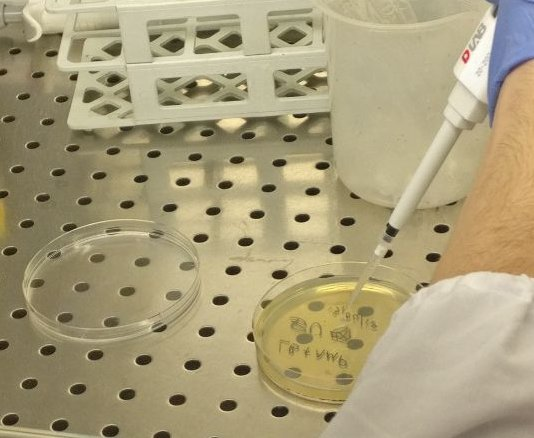
\includegraphics[width=0.6\textwidth]{./immagini/piastraggio_colonie.jpg}
		\caption{Piastraggio delle cellule di E. Coli su terreno LB-Amp}
		\label{piastraggio cellule}
	\end{figure}
\end{enumerate}

\subsection{Risultati e Conclusioni}

Tramite questa procedura abbiamo potuto inserire all'interno delle nostre cellule batteriche
di E.coli i plasmidi pUC18 rendendole competenti, permettendoci cos\`i di clonare od esprimere
i geni di interesse.

	\newpage

	%_______________________________ESPERIENZA N° 7 (ALLESTIMENTO COLTURE CELLULARI)
	\chapter{Allestimento di colture cellulari}

\vspace{0.6cm}

\section{Sommario}

\subsection{Scopo}

Quest'esperienza in laboratorio ha come scopo l'allestimento di una coltura cellulare
su un Multiwell plate per poter effettuare esperimenti.

\subsection{Cenni teorici}

La creazione di colture cellulari \`e tra le attivit\`a pi\`u comuni e importanti
effettuate in un laboratorio di biologia molecolare. Le colture permettono di
far replicare le cellule, facilitando l'estrazione di RNA, DNA e proteine oltre a
permettere la selezione delle cellule trasformate grazie all'aggiunta di antibiotico
al terreno.

\subsection{Materiali utilizzati}

\begin{itemize}
	\item Guanti in lattice
	\item Falcon da 50ml
	\item Cell-scraper
	\item Flask con cellule
	\item Centrifuga
	\item Multiwell plate
\end{itemize}

\subsection{Soluzioni utilizzate}

\begin{itemize}
	\item PBS
	\item Terreno DMEM
	\item FBS
	\item Cocktail di antibiotici-antimicotici
\end{itemize}

\section{Procedimento}

\subsection{Preparazione del terreno di coltura}

\begin{itemize}
	\item Aliquotare 10ml di terreno DMEM sotto cappa sterile
	(per evitare contaminazioni) in Falcon da 50ml.
	\item Supplementare il terreno aggiungendo il 10\% di FBS.
	Il siero fetale bovino \`e necessario per fornire alle cellule sostanze non
	presenti nel terreno di coltura, come proteine plasmatiche,
	fattori di crescita, chelanti, vitamine ed elettroliti.
	\item Aggiungere cocktail di antibiotici-antimicotici in concentrazione 1\%
	c\`o permette la selezione dei batteri trasformati dai plasmidi
\end{itemize}

\subsection{Staccare le cellule mediante cell-scraper}
\begin{itemize}
	\item Eliminare il terreno esausto.
	\item Lavare con 5ml di PBS, agitando delicatamente.
	\item Ripetere il lavaggio con PBS.
	\item Bagnare tutta la superficie della flask con 10ml di PBS e staccare
	delicatamente le cellule con lo scraper. Se viene esercitata troppa forza le
	cellule rischiano di lisarsi.
	\item Prelevare le cellule in PBS e spostarle in una Falcon da 15ml.
	\item Centrifugare per 15' a 500g.
\end{itemize}

\subsection{Spostare le cellule nel Multiwell plate}
\begin{itemize}
	\item Una volta ottenuto il pellet eliminare il surnatante sotto cappa sterile.
	\item Risospendere il pellet in 1,5ml di terreno completo.
	\item Aliquotare 500$\mu$l di cellule per pozzetto.
	\item Riempire i pozzetti.
\end{itemize}

\section{Risultati e Conclusioni}

Durante questa esperienza abbiamo imparato a creare un terreno di coltura
e spostare le cellule in esso, tramite l'utilizzo del cell-scraper.
Abbiamo inoltre visto come utilizzare il Multiwell plate come supporto per la
nostra coltura.

	\newpage

	%_______________________________ESPERIENZA N° 8 (UTILIZZO COLTURE UMANE)
	\chapter{Utilizzo delle colture cellulari umane in analisi molecolari e morfologiche}

\vspace{0.6cm}

\section{Sommario}

\subsection{Scopo}

In questa esperienza sono state utilizzate delle colture cellulari
di melanoma umano.
Queste colture saranno usate per la raccolta dell'RNA e l'analisi proteica.
Una terza coltura è stata colorata con un colorante viola per poter
osservare al microscopio le cellule.

\subsection{Cenni teorici}

Le colture cellulari sono molto importanti per poter studiare le cellule durante
il loro ciclo vitale, e per amplificare DNA, RNA e proteine semplificandone l'estrazione.

\subsection{Strumenti e materiali utilizzati}

\begin{itemize}
\item Guanti in lattice
\item Pasteur in plastica monouso
\item Cell scraper
\item Falcon da utilizzare come scarto
\item Provette Eppendorf (2mL)
\item Micropipette (\SI{100}{\micro\liter}-\SI{1000}{\micro\liter} e \SI{2}{\micro\liter}-\SI{200}{\micro\liter})
\item Microscopio ottico
\end{itemize}

\subsection{Soluzioni utilizzate}

\begin{itemize}
\item Cristalvioletto in eppendorf da 1,5ml
\item RNAlater in eppendorf da 1,5ml
\item 5ml PBS 10X + 45ml ddH$_2$O, in provetta Falcon 50ml
\end{itemize}

\section{Procedimento}

\subsection{Raccolta cellule per analisi proteica}

\begin{enumerate}

\item Aspirare completamente il terreno di coltura con la pasteur.
\item Aggiungere con la pasteur 1ml di PBS, riaspirarlo con quest'ultima e scartarlo.
\item Ripetere la procedura precedente.
\item Aggiungere 1,5ml di PBS.
\item Staccare le cellule con il cell scraper.
Dopo averlo utilizzato lo conserviamo nel fodero per riutilizzarlo successivamente
Per staccare le cellule con questo strumento, muovere esercitando una leggera pressione
e spostarsi lungo tutta la superficie.
\item Aspirare 1,5ml di PBS con le cellule in sospensione e trasferire su una eppendorf da 2ml
\item Centrifugare per 10 minuti a 10.000g.
\item Adesso tutte le cellule si trovano sul fondo formando un pellet. Aspirare tutto
i PBS sopranatante facendo attenzione a non staccare il pellet.
\item Conservare a -20°C per la successiva estrazione delle proteine.

\end{enumerate}

\subsection{Raccolta cellule per raccolta RNA}

\begin{enumerate}
    \item Aspirare completamente il terreno di coltura con la pasteur.
    \item Aggiungere con la pasteur 1ml di PBS, riaspirarlo con quest'ultima e scartarlo.
    \item Ripetere la procedura precedente.
    \item Aggiungere 1ml di RNAlater.
    \item Staccare le cellule con il cell scraper.
    \item Aspirare tutto l'RNAlater con le cellule in sospensione e portarlo su una
    eppendorf da 2ml.
    \item Centrifugare per 10 minuti a 10.000g.
    \item Adesso tutte le cellule si trovano sul fondo formando un pellet. Aspirare tutto
    i PBS sopranatante facendo attenzione a non staccare il pellet.
    \item Conservare a -20°C per la successiva estrazione degli acidi nucleici.
\end{enumerate}

\subsection{Colorazione del tappeto cellulare}

\begin{enumerate}
    \item Aggiungere sotto cappa chimica 1ml di formalina al pozzetto delle cellule da
    colorare e lasciare agire per 20/30 minuti.
    \item Spostarsi sul bancone e aspirare tutto il liquido con la pasteur e scartarlo.
    \item Aggiungere 1ml di PBS con la pasteur, riaspirarlo con quest'ultima e scartarlo.
    \item Ripetere la procedura con il PBS.
    \item Aggiungere con la pasteur tutto il cristalvioletto contenuto nell'aliquota fornita
    (1ml) facendo attenzione a non sporcarsi.
    \item Lasciare agire il colorante per 30 minuti, dopodich\`e aspirarlo e scartare il colorante.
    \item Aggiungere 1ml di PBS con la pasteur, aspirarlo con quest'ultima e scartarlo.
    \item Ripetere questa procedura altre 3/4 volte per lavare il colorante e poterle visualizzare
    al microscopio.
    \item Aggiungere 1ml di PBS nel pozzetto colorato, ora si possono osservare al
    microscopio le cellule colorate.
\end{enumerate}

\section{Risultati e Conclusioni}

In figura vediamo le cellule di melanoma colorate di viola (le sagome irregolari, normalmente non visibili).
Sono inoltre presenti dei puntini viola che corrispondono a dei vacuoli che si sono colorati.

\begin{figure}[htbp]
	\centering
	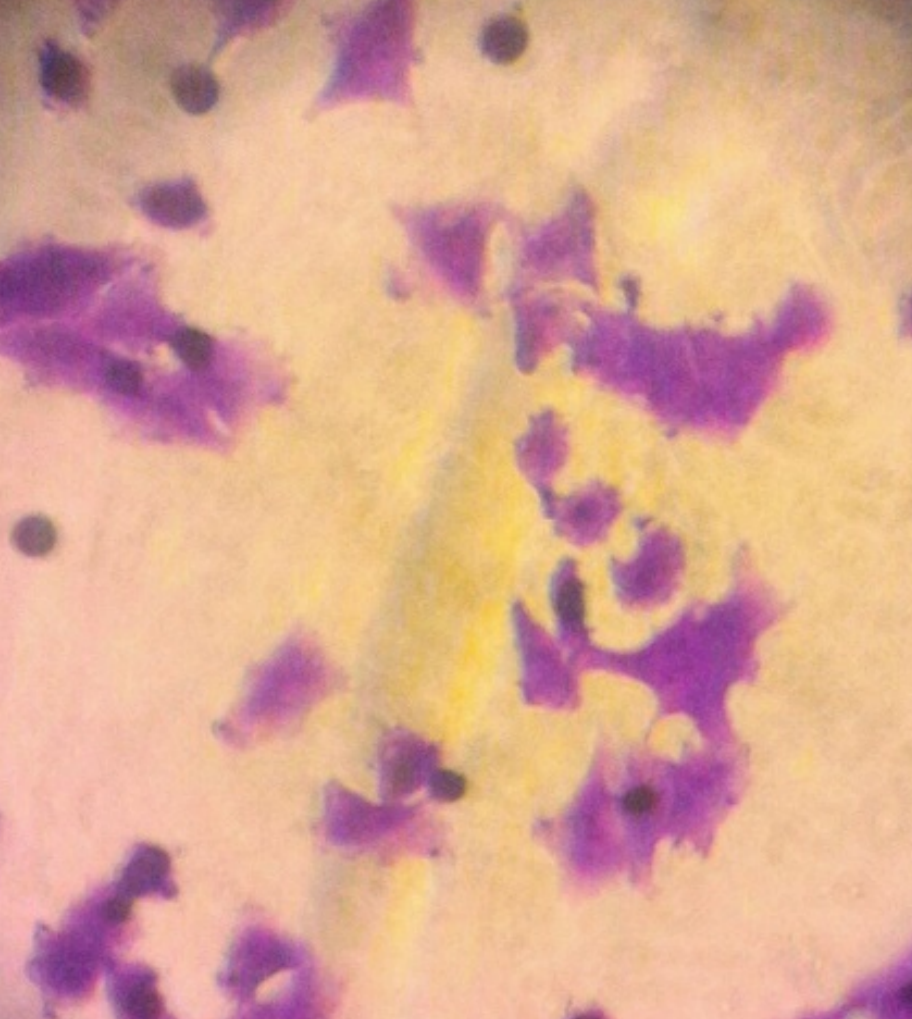
\includegraphics[width=80mm]{./immagini/melanoma.png}
	\caption{Risultati colorazione}
	\label{melanoma}
\end{figure}

	\newpage

	%_______________________________ESPERIENZA N° 10 (REAL TIME PCR)
	\section{\LARGE{Amplificazione RealTime PCR. Estrazione proteine totali }}

\vspace{0.6cm}

\subsection{Sommario}

\subsubsection{Scopo}

In questa esperienza vediamo due procedimenti:
\begin{itemize}
  \item Amplificazione di un cDNA tramite la PCR real time.
  \item L'estrazione delle proteine e la loro quantificazione al Qubit 3.
\end{itemize}

\subsubsection{Cenni teorici}

La PCR real time è una particolare PCR che ci permette di amplificare e
contemporaneamente quantificare il DNA in tempo reale osservando la fluorescenza
ad ogni iterazione.
%Paragonando due campioni diversi \`e possibile stabilire il rapporto tra le quantit\`a
%iniziali della sostanza.
Per rendere il campione fluorescente si utilizza una sonda composta da un colorante
fluorescente (Responser) e da un Quencer che assorbe l'energia della fluorescenza.
La sonda si lega tra i due primer (forward e reverse) del gene.
Quando la sonda viene degradata (dall'attivita' esonucleasica della TAQ-polimerasi)
il Quencer e il Responser si separano. In questo modo il Responser e' libero di emettere
fluorescenza che risulta visibile e misurabile.

\subsubsection{Strumenti e materiali utilizzati}

\begin{itemize}
\item Guanti in lattice
\item Provette Eppendorf (1.5ml)
\item Assay tube (500$\mu$l)
\item Micropipette (100-1000  e 2-200 $\mu$l)
\item Qubit 3 (per quantificare le proteine)
\end{itemize}

\subsubsection{Soluzioni utilizzate}
\begin{itemize}
\item cDNA
\item Pellet cellulare per l'estrazione delle proteine
\item RIPA buffer (soluzione tampone utilizzata per l'estrazione di proteine da cellule
di mammifero)
\item Working solution
\end{itemize}

\subsection{Procedimento}

\subsubsection{Amplificazione RealTime PCR}
\begin{itemize}
\item Prendere il cDNA dall'esperienza precedente
\item Utilizzare questa quantit\`a di reagenti per un volume finale di 40$\mu$l diviso in
due pozzetti da 20$\mu$l: \\
\begin{tabular}{c c c c}
\hline
Reagente & Concentrazione & $\mu$l/pozzetto & $\mu$l 2 pozzetti \\
\hline
MasterMix & 2X & 10$\mu$l & 20$\mu$l \\
Sonda TaqMal & 20X & 1$\mu$l & 2$\mu$l \\
H$_2$O & 1X & 7$\mu$l & 14$\mu$l \\
cDNA & 1X & 2$\mu$l & 4$\mu$l \\
\end{tabular}
\item Aliquotare ogni reagente in un'eppendorf da 1,5ml.
\item Spostare ogni reazione nei pozzetti (appoggiarsi al bordo per essere pi\`u precisi)
\item Sigillare con l'adesivo ottico
\item Centrifugare brevemente
\item Avviare la reazione di amplificazione \\
Questi sono i parametri del termociclatore:\\
\begin{tabular}{c c c c c}
\hline
Parametro & Incubazione UNG & Attivazione polimerasi &
\multicolumn{2}{c}{PCR (40 cicli)} \\
\hline
& Hold & Hold & Denaturazione & Annealing/estensione \\
\hline
Temperatura & 50C & 95C & 95C & 60C \\
\hline
Tempo (mm:ss) & 02:00 & 10:00 & 00:15 & 01:00 \\
\end{tabular}
\item Attendere il completamento ed analizzare i dati raccolti
\end{itemize}

\subsubsection{Estrazione delle proteine}
\begin{itemize}
\item Risospendere il pellet cellulare in 100ul di RIPA Buffer addizionato
di inibitori di proteasi con la diluizione: \\
\begin{tabular}{c c c}
Reagente & Concentrazione & Quantit\`a \\
RIPA buffer & 1X & 96ul \\
Inibitori & 25X & 4ul \\
& & TOT = 100$\mu$l \\
\end{tabular}
Il buffer di lisi serve a rompere le cellule.

\item Incubare per 45' in ghiaccio
\item Centrifugare per 40'' a 4°C
\item Prelevare il surnatante (contenente le proteine) in una nuova eppendorf
\item Conservare in ghiaccio
\end{itemize}

\subsubsection{Quantificazione proteine con Qubit 3}
\begin{itemize}
\item Preparare la Working Solution, che servir\`a sia per la taratura dello strumento
che per la misurazione della quantit\`a di proteine. Nel nostro caso lo strumento era
gi\`a stato tarato, quindi dalla tabella escludiamo le 3 dosi per la taratura.

\begin{tabular}{c c c}
Reagente & Quantit\`a 1 dose & Quantit\`a 10 dosi \\
Qubit protein reagent & 1ul & 10ul \\
Qubit protein buffer & 199ul & 1990ul \\
 & TOT = 200ul & TOT = 200ul \\
\end{tabular}

\item Aliquotare 190$\mu$l di Working Solution in un AsseyTube da 500$\mu$l
\item Aggiungere 10$\mu$l di proteine, invertire il tubo 10 volte e centrifugare brevemente
\item Lasciare la miscela al buio per 15'
\item Leggere l'emissione del fluoroforo

\end{itemize}

\begin{figure}[H]

	\centering
	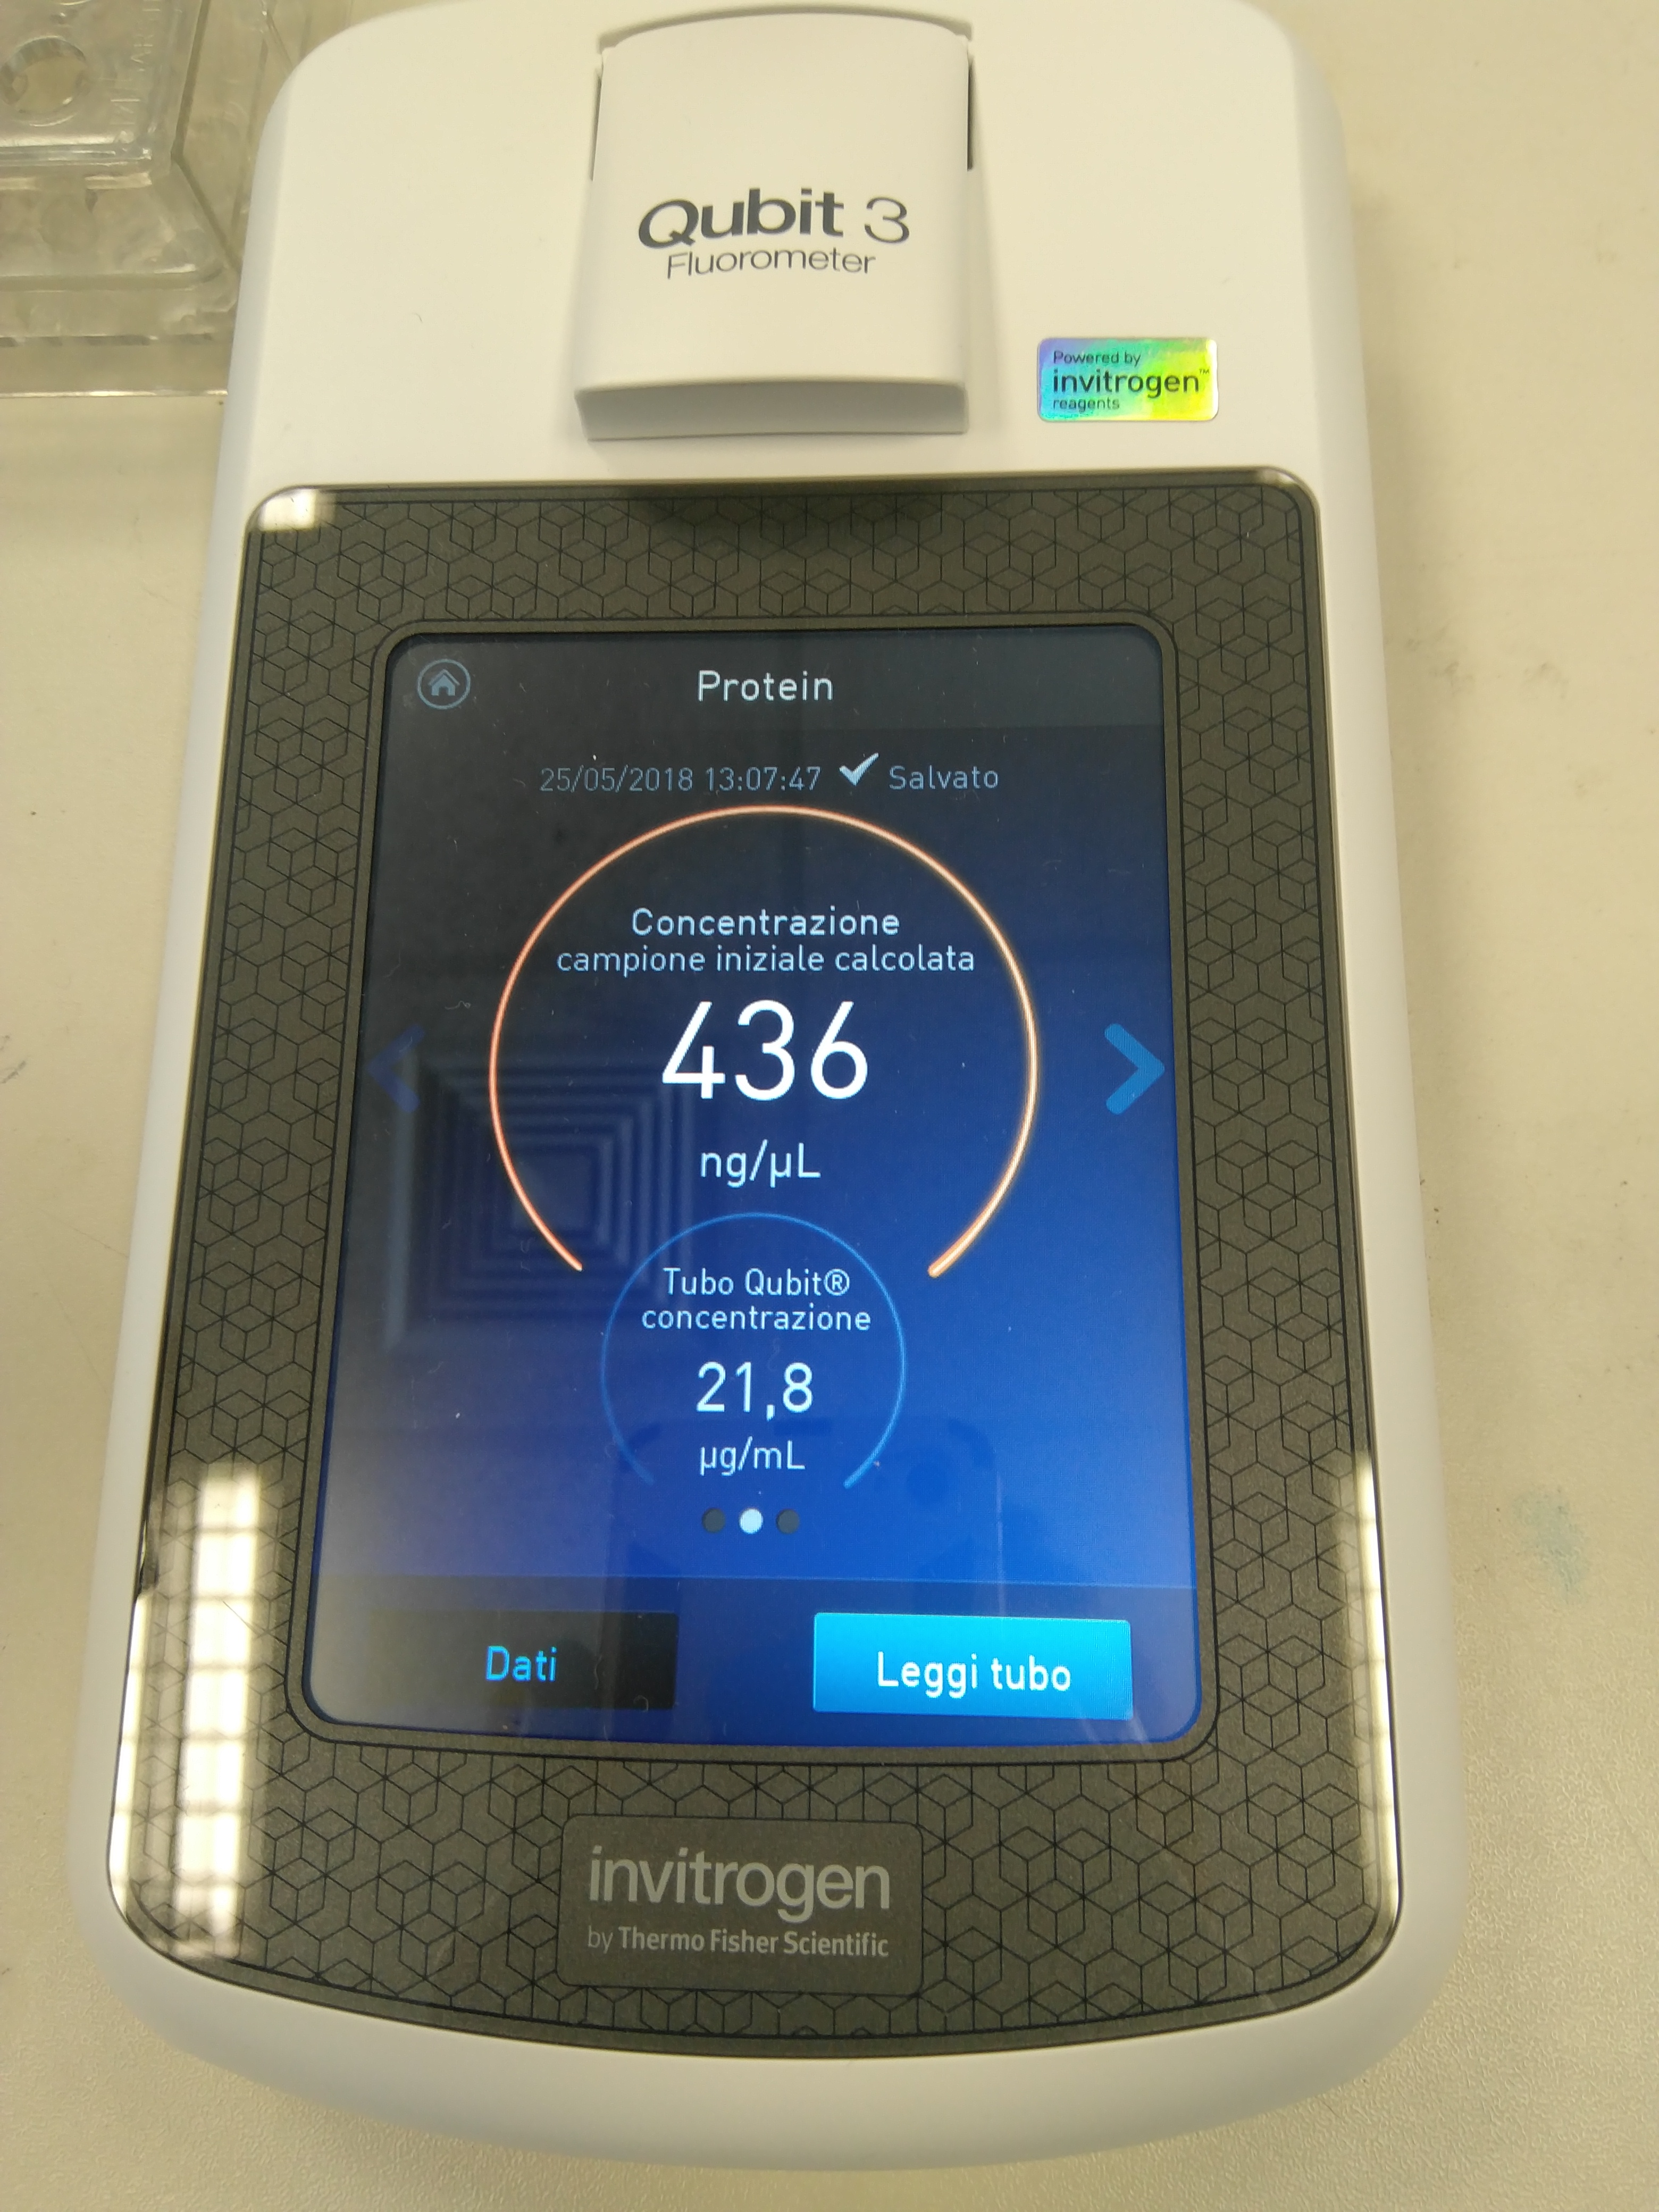
\includegraphics[width=0.4\textwidth]{./immagini/qubit3.jpg}
	\caption{Risultati della quantificazione delle proteine.}
	\label{fig:qubit3}

\end{figure}

\subsection{Risultati e Conclusioni}

\begin{itemize}
\item RealTime PCR:
Come risultato abbiamo osservato un grafico con una curva di amplificazione
con le quantit\`a ad ogni ciclo.
Abbiamo visto che ha un andamento logaritmico.
Tracciando una linea orizzontale e' possibile verificare la soglia di fluorescenza.\\

\item Quantificazione Proteine:
La concentrazione ottenuta per le nostre proteine e' di 436 ng/ul. Visto che eravamo partiti con una
quantita' di 100ul, e 10ul sono stati utilizzati per la quantificazione, moltiplicando per 90ul possiamo
ottenere la quantita' totale di proteine del nostro campione.
\end{itemize}

	\newpage

	%_______________________________ESPERIENZA N° 11 (ELETTROFORESI SDS-PAGE)
	\section{\LARGE{Elettroforesi SDS-PAGE}}

\vspace{0.6cm}


\subsection{Sommario}

\subsubsection{Scopo}

Lo scopo di questa esperienza e' effettuare l'elettroforesi
delle proteine estratte nell'esperienza 10 tramite la
tecnica SDS-PAGE.

\subsubsection{Cenni teorici}

Solitamente l'elettroforesi ha la capacit\`a di separare le proteine secondo sia
la carica che la massa.
L'elettroforesi SDS-PAGE, che si effettua in gel di acrilammide, si differenzia
rispetto ad altre procedure in quanto la separazione delle proteine
avviene solo in base al solo peso molecolare, indipendentemente dalla carica.
Ci\`o \`e possibile grazie alla propriet\`a denaturante dell'SDS,
che permette di mantenere costante il rapporto massa-carica per ogni proteina denaturata.
L'SDS, acronimo di Laurilsolfato di sodio, e' un tensioattivo in grado di denaturare le proteine e
caricarle negativamente in modo proporzionale alla loro massa.

Il gel e' diviso in due parti, stacking gel e running gel. Lo stacking gel
ha lo scopo di allineare le proteine, portandole tutte allo stesso livello e per
questo contiene una percentuale minore di acrilammide.
Il running gel ha invece il compito di permettere alle proteine di separarsi a
seconda della carica.

\subsubsection{Strumenti e materiali utilizzati}

\begin{itemize}
\item Guanti in lattice
\item Provette Eppendorf (2ml)
\item Micropipette (100-1000 e 2-200 ml)
\item Falcon (50mL)
\item Carta bibula
\item Apparato per casting del gel elettroforetico
\end{itemize}

\subsubsection{Soluzioni e composti}

\begin{itemize}
\item Laemmli Sample Buffer 4X
\item Acrilammide/bis
\item 1,5M Tris-HCl, pH 8,8
\item Tris base
\item Glicina
\item 10\% soluzione SDS
\item 10\% ammonio persolfato
\item TEMED
\item isopropanolo
\item ddH20
\item Proteine da analizzare 20ug (estratte nell'esperienza 10)
\item Tris base
\item Glicina
\item 10\% soluzione SDS
\end{itemize}


\subsection{Procedimento}

\subsubsection{Preparazione del Running/Resolving gel}

\begin{tabular}{|l|l|l|} \hline
	& \textbf{Concentrazione} & \textbf{Quantit\'a} \\\hline
	Acrilammide/bis & 40\% & 3,2ml \\\hline
	1,5M Tris-HCl, pH 8,8 & 25\% & 2,0ml \\\hline
	SDS soluzione 10\% & 1\% & 0,8ml \\\hline
	Ammonio persolfato 10\% & 1\% & 0,8ml \\\hline
	TEMED & 0,1\% & 0,08ml \\\hline
	ddH$_2$O & \multicolumn{2}{c|}{a volume totale} \\\hline

	& \textbf{TOTALE} & 300ml \\\hline
\end{tabular}

\begin{enumerate}
	\item Predisporre l'apparato necessario al casting del gel elettroforetico.

	\item Miscelare tutti i componenti della tabella 1 in una Falcon da 50mL.

	\item Distribuire velocemente la miscela tra i vetri dell'apparato, \`e importante
	tenere l'eccesso del gel all'interno della Falcon, per stabilire quando il gel
	si sar\`a solidificato.

	\item Stratificare sino a riempimento con alcol isopropilico.
	Questa fase \`e necessaria per limitare il contatto con l'aria
	del gel che si sta solidificando e contemporaneamente	permettere
	un livellamento del gel grazie al peso dell'alcol.
	\`E importante notare che in questa fase l'alcol e
	il gel non si mescolano.

	\item Attendere la polimerizzazione (confermata dalla quantit\`a di
	gel lasciata nella Falcon)
\end{enumerate}

\subsubsection{Preparazione dell'Electrode Running Buffer 10X}
\begin{itemize}
	\item Preparare l'Electrode Running Buffer utilizzando
	le seguenti soluzioni:\\
	\begin{tabular}{|l|l|l|} \hline
		& \textbf{Concentrazione} & \textbf{Quantit\'a} \\\hline
		Tris base & 3\% & 9ml \\\hline
		Glicina & 14,4\% & 43,2ml \\\hline
		SDS soluzione 10\% & 1\% & 3ml \\\hline
		& \textbf{TOTALE} & 300ml \\\hline
	\end{tabular}
\end{itemize}

\subsubsection{Preparazione dello stacking gel}

\begin{tabular}{|l|l|l|} \hline
	& \textbf{Concentrazione} & \textbf{Quantit\'a} \\\hline
	Acrilammide/bis & 61\% & 3,05ml \\\hline
	1,5M Tris-HCl, pH 8,8 & 25\% & 1,25ml \\\hline
	10\% soluzione SDS & 1\% & 0,05ml \\\hline
	10\% ammonio persolfato & 1\% & 0,05ml \\\hline
	TEMED & 0,2\% & 0,01ml \\\hline
	ddH20 & \multicolumn{2}{c|}{a volume totale} \\\hline
	& \textbf{TOTALE} & 5ml \\\hline
\end{tabular}

\begin{itemize}
	\item Miscelare tutti i componenti della tabella in una Falcon
	da 50ml.
	\item Aliquotare rapidamente la miscela tra i vetri del gel, tenendo
	l'eccesso nella Falcon per confronto.
	\item Inserire il pettine per permettere la formazione dei pozzetti
	di caricamento.
	\item Attendere la polimerizzazione del gel.
\end{itemize}

\subsubsection{Posizionamento dello stacking gel}
% \begin{enumerate}


	% \begin{figure}[H]
	% 	\centering
	% 	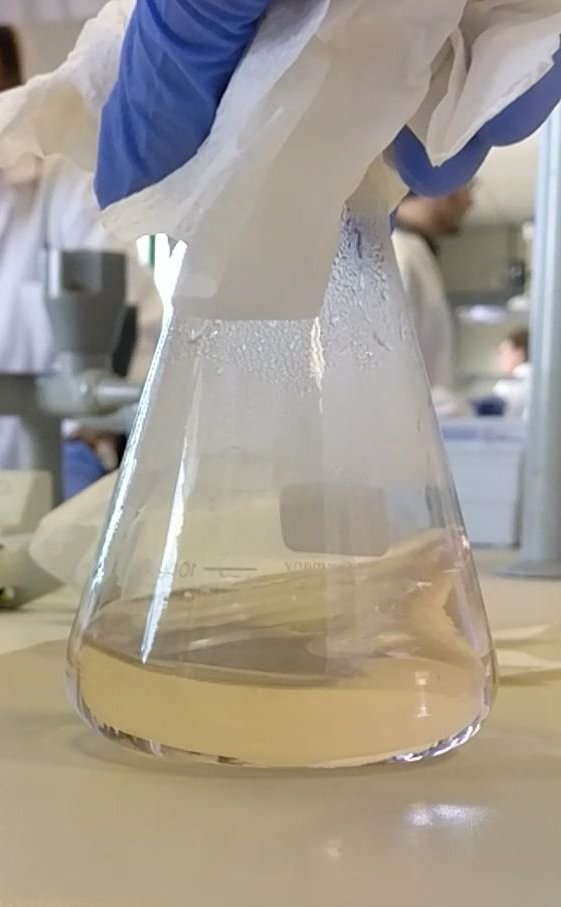
\includegraphics[width=0.3\textwidth]{./immagini/agarosio.jpg}
	% 	\caption{Mescolamento della soluzione con agarosio}
	% 	\label{agarosio}
	%
	% \end{figure}


% \end{enumerate}
\subsubsection{Colorazione del gel}
\begin{itemize}
\item Smontare i vetri che racchiudono il gel di corsa.
\item Lavara i gel per 3 volte da 5' ciascuna in ddH$_2$O.
\item Porre i gel in 10ml di Comassie Blue Staining.
\item Lasciar colorare per circa 1h.
\item Lavare i gel 5 volte in ddH$_2$O.
\end{itemize}


\subsection{Risultati e Conclusioni}

In questa esperienza abbiamo imparato come svolgere una tecnica
molto utilizzata in biologia molecolare, che permette la separazione
delle proteine in base alla loro massa.
Purtroppo nel nostro caso, a causa di un errore di concentrazione
dell'Electrode Running Buffer, non \`e stato possibile ottenere
risultati soddisfacenti.

	\newpage

	%_______________________________ESPERIENZA N° 12 (SEPARAZIONE CELLULARE SU GRADIENTE DI FICOLL)
	\chapter{Separazione cellulare su gradiente di ficoll}

\vspace{0.6cm}

\section{Sommario}

\subsection{Scopo}

In questa esperienza introduciamo la metodologia di separazione per le cellule del sangue.
Questa operazione viene effettuata per purificare linfociti e monociti,
separandoli dai globuli rossi e dai granulociti (esempio piastrine) che sono di gran
lunga i componenti più numerosi del sangue.\\
Considerazione: essendo che non possiamo lavorare con il sangue in quanto può
essere molto rischioso abbiamo usato delle cellule di melanoma prese da una coltura.


\subsection{Cenni teorici}
Questa procedura viene usata specialmente per il sangue.
Essa permette di isolare le sue diverse componenti in modo tale da poter successivamente
lavorare più nello specifico con quelle di nostro interesse.\\
Un ruolo importante lo riveste il Ficoll.
Il Ficoll è un copolimero sintetico di alto peso molecolare e grazie alla sua densità
permette di spingere verso il fondo quelle componenti che non ci interessano.
Quindi nel caso del sangue otterremo 4 diverse fasi:
\begin{figure}[H]
    \centering
    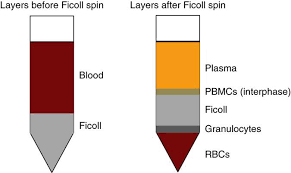
\includegraphics{./immagini/Ficoll_sangue.png}
    \caption{Falcon con sangue pre e post centrifuga}
\end{figure}

\section{Materiali utilizzati}

\begin{itemize}
\item Guanti in lattice
\item Provette Eppendorf (1.5 mL)
\item Falcon da 15 ml
\item Falcon da 50ml
\item Camera di Burker
\item Centrifuga
\item Micropipetta (\SI{100}{\micro\liter}-\SI{1000}{\micro\liter})

\end{itemize}

\section{Soluzioni utilizzate}

\begin{itemize}

\item PBS
\item Tripsina
\item Wash Buffer (terreno di coltura contenente FBS)
\item FBS
\item Ficoll

\end{itemize}

\section{Procedimento}

\subsection{Preparazione della sospensione cellulare}

\begin{enumerate}

    \item Eliminare il terreno di coltura

    \item Lavare le cellule con 20 ml di PBS; eliminare il liquido di lavaggio

    \item Ripetere il lavaggio con ulteriori 20 ml di PBS; eliminarlo

    \item Addizionare 5 ml di tripsina; lasciare incubare per 5' a 37°C.
    La tripsina permette di staccare le cellule in modo non meccanico (senza cell scraper).

    \item Addizionare alla tripsina 15 ml di Wash Buffer (terreno di coltura con FBS).

    \item Centrifugare a 300g per 10' RT.

    \item Risospendere in 50 ml di Wash Buffer.

    \item A 5 ml di sospensione aggiungere ulteriori 5 ml di Wash Buffer portando
    ad un volume di 10 ml totali.

\end{enumerate}

\subsection{Allestimento separazione su gradiente}

\begin{enumerate}
    \item Diluire il PBS 10X e prelevarne 50 ml 1X in una falcon da 50 ml.
    \item Aliquotare su una Falcon da 15 ml 4 ml di Ficoll.
    \item Stratificare molto lentamente, mediante l'utilizzo di una Pasteur monouso,
    la sospensione di cellule; bisogna far attenzione a non agitare per non compromettere
    la stabilità della deposizione su Ficoll.
    \item Centrifugare per 30' a 800 g RT senza accelerazione nè freno.
    \item Dopo la centrifuga si ottiene una separazione su gradiente che isolerà le cellule
    formando un anello in base alla loro densità. Otteniamo nel nostro caso solo una fase,
    ma nel caso del sangue si vedrebbero diverse fasi che rappresentano le varie componenti.
    \item Prelevare l'anello di cellule formatosi tra il Ficoll e il liquido si sospensione
    cellulare facendo particolare attenzione in quanto è un passaggio delicato.
    Prelevato l'anello spostarlo in una Falcon da 15 ml.
    \item Riempire per decantazione la Falcon di PBS portandolo a un volume finale di 15 ml.
    \item Centrifugare a 400g per 10'; finita la centrifuga scartare il surnatante
    e risospendere il pellet di cellule.
    \item Aggiungere per decantazione ulteriore PBS e portarlo a un volume di 10 ml.
    \item Centrifugare nuovamente a 400 g per 10'; finita la centrifuga scartare di nuovo
    il surnatante e risospendere in 1ml di PBS con la micropipetta da 100 $\mu$.
    \item Spostare infine su una eppendorf da 1.5 ml.
\end{enumerate}

\subsection{Conta cellulare su camera contaglobuli di Burker}
\begin{enumerate}
    \item Diluire le cellule 1:10 in $\mu$ finali su nuova eppendorf.
    \item Montare la camera di Burker.

    \begin{figure}[H]
    \centering
    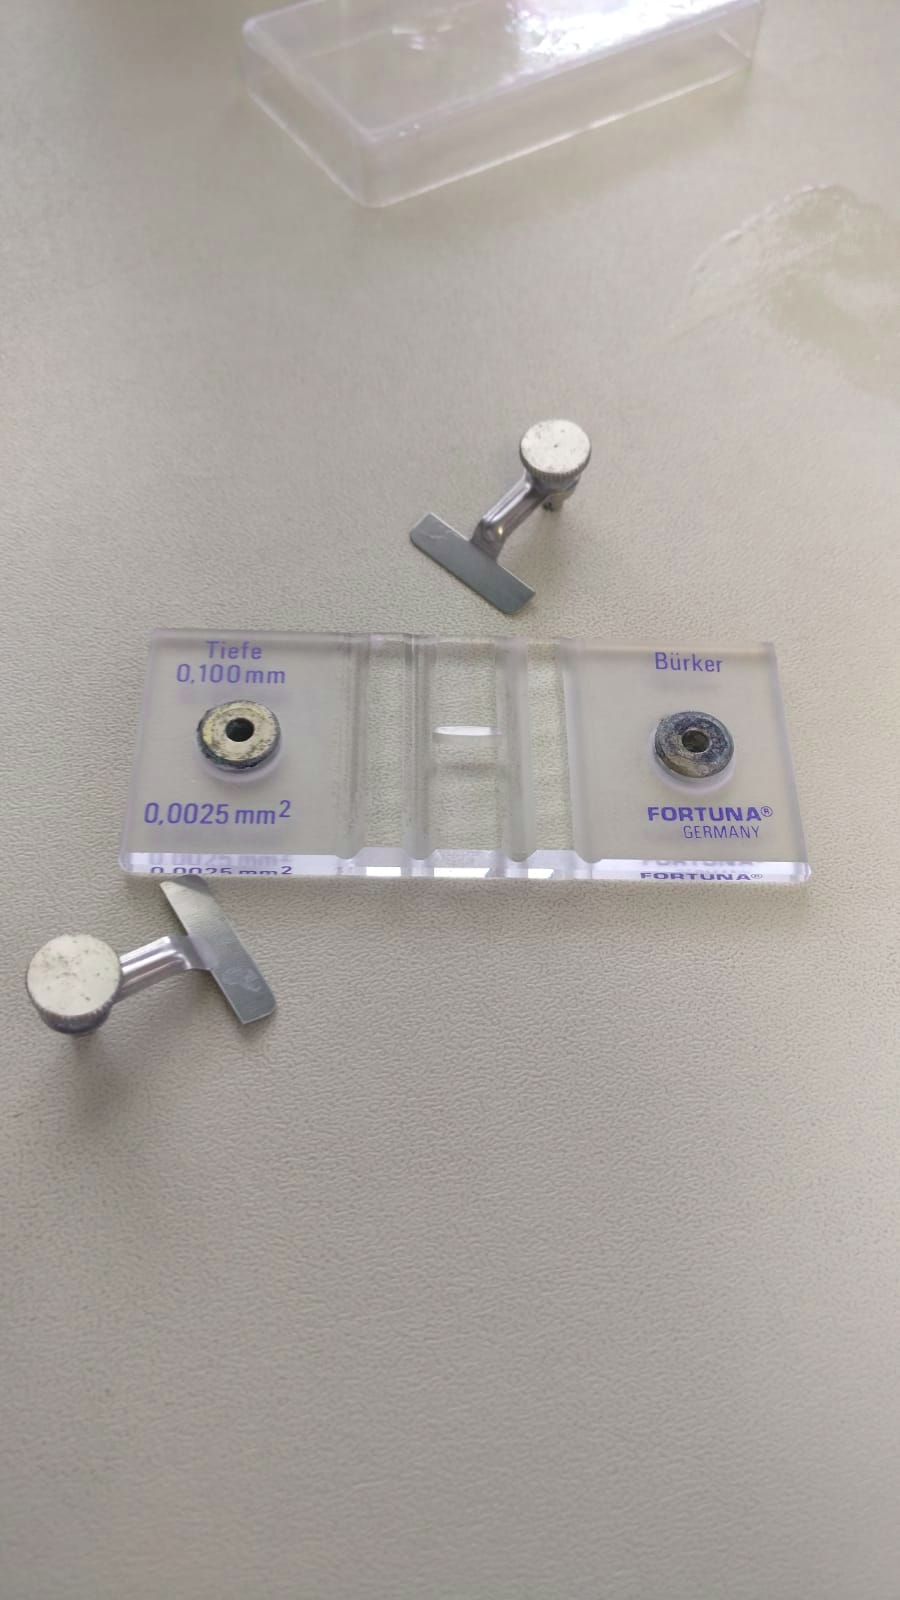
\includegraphics[width = 0.4\textwidth]{./immagini/Burker.png}
    \caption{Burker}
    \end{figure}

    \item Riempire i due pozzetti della camera per capillarità mediante l'utilizzo di
    una pipetta da 200 $\mu$l. Capiamo che la camera è piena quando da sotto il
    copri-vetrino uscirà una goccia.
    \item Contare le cellule comprese all'interno del quadrato che presenta come bordo 3
    righe.
\end{enumerate}

\section{Risultati e Conclusioni}

Il numero di cellule da noi trovate è 92. Un numero così elevato è stato ottenuto per la
non diluizione specificata precedentemente. \\
Il totale delle cellule diluite si sarebbe ottenuto con questa formula :
    $$[cellule] = (num. cellule)*(fatt. diluzione)*(fatt. moltiplicativo camera)$$
Nel nostro caso il fattore moltiplicativo della camerà è 10000.

\end{document}

	\newpage

\end{document}
